\typeout{Informative Seafloor Exploration with Linearised Differential Entropy of Gaussian Process Classifiers}
\documentclass{article}
\usepackage{acra}

%%%%%% Kelvin's Packages %%%%%% 
\usepackage{vector}  % Allows "\bvec{}" and "\buvec{}" for "blackboard" style bold vectors in maths
\usepackage{bm}
\usepackage{amsmath}
\usepackage{amssymb}
\usepackage{graphicx}
\usepackage{psfrag}
\usepackage{epstopdf}
\usepackage{tikz}
\usepackage{smartdiagram}
\usepackage{upgreek}
\usepackage{stfloats}

\renewcommand{\vec}[1]{\boldsymbol{#1}}
\newcommand\numberthis{\addtocounter{equation}{1}\tag{\theequation}}
\newcommand{\incite}[1]{\citeauthor{#1} [\citeyear{#1}]}

\title{Informative Seafloor Exploration using the Linearised Differential Entropy of Gaussian Process Classifiers}
\author{Kelvin YS Hsu\textsuperscript{\textnormal{12}}, Simon O'Callaghan\textsuperscript{\textnormal{1}}, Alistair Reid\textsuperscript{\textnormal{1}}, Stefan B Williams\textsuperscript{\textnormal{2}} \\ National ICT Australia\textsuperscript{1} \\ Australian Centre for Field Robotics, University of Sydney\textsuperscript{2} \\ 
\{Kelvin.Hsu, Simon.Ocallaghan, Alistair.Reid\}@nicta.com.au, s.williams@acfr.usyd.edu.au}

\begin{document}

\maketitle

\begin{abstract}
	While seafloor bathymetry have been mapped extensively over the last few decades, geological and ecological observations of seafloor benthic zones only began recently. Unlike bathymetric mapping, data collection of benthic imagery requires \textit{in situ} exploration - a significantly slower and costly endeavour. An efficient exploration policy would therefore require solving the informative path-planning problem. This paper investigates a receding horizon approach to the informative path-planning problem using linearised differential entropy as the proposed acquisition function. We model the benthic environment using five bathymetric features through Gaussian process classifiers, whose linearised differential entropy (LDE) would be defined and derived. We demonstrate that LDE acquisition achieves the lowest misclassification rate under a receding horizon formulation, outperforming acquisition under both Monte Carlo based joint information entropy and marginalised information entropy. In particular, it avoids the time complexity of Monte Carlo sampling, while still retaining a measure of mutual information. We also show the benefits of a receding horizon approach over simpler techniques such as greedy and open loop methods. Finally, we test our method on collected benthic datasets from past AUV missions to Scott Reef, Western Australia.
\end{abstract}

\section{Introduction}
\label{Section:Introduction}

	Today, less than five percent of the ocean have been explored \cite{NOAA}. As the ocean covers more than 70\% of the globe, this leaves more than 67\% of the planet's habitats unexplored despite our deep reliance on much of these undiscovered ecosystems.
	
	In order to understand the ecological, geological, chemical, and archaeological aspects of the ocean floor, autonomous underwater vehicles (AUVs) are now capable of efficiently collecting information and observations from natural environments of large spatial scale. In the case of benthic habitat mapping, AUVs collect imagery data of seafloor environments. However, it is impractical and often infeasible to identify semantic meaning from the images with human experts. Instead, visual data are clustered into benthic labels that summarises the corresponding benthic environment. For example, \incite{Steinberg2015128} uses Gaussian latent Dirichlet allocation (LDA) to perform unsupervised clustering of benthic imagery, releasing the burden on human experts to analyse collected imagery exhaustively and thus remove a significant bottleneck in the habitat mapping process.

	Nevertheless, the immense spatial scale of the benthic seafloor to be explored implies that it is impractical to map exhaustively the entire region of interest (ROI) under any reasonable time and cost. Furthermore, AUV missions are limited by power supply, data storage, and computational capabilities. As such, AUVs must prioritise exploring sub-domains of the ROI that ideally contain the most important and valuable information.
	
	Thus, practical seafloor exploration must employ an inference model that allows the AUV to quantify the expected amount of information at a given region or location. To perform such an inference, we model the habitat classes onto bathymetric features that summarises the local depth and seafloor structure using a Gaussian process classifier.

	Gaussian process (GP) models are non-parametric, Bayesian inference models which make relatively few assumptions onto the type of phenomena to be inferenced as compared to parametric models. In contrast to non-Bayesian methods, GPs handles uncertainty inherently in its model and is thus an excellent framework for informative inference. Under the class of radial basis function (RBF) kernels, the primary inference philosophy behind GP models are that the proximity of observations in feature space determines their corresponding correlation. In the benthic context, this translates to the underlying assumption that the type of habitat at a particular location depends strongly on the local bathymetric structure.
		
	Once the AUV is able to quantify the expected amount of information at a given location, it is natural to consider the paths the AUV could take to maximise information gain over its mission, thus achieving efficient habitat mapping. As such, we employ an informative path-planning policy to navigate through paths that contain the most valuable information regarding the ROI. 
	
	This paper addresses the informative path-planning problem for benthic habitat mapping. Due to the limited computational resources available for \textit{in-situ} exploration with AUVs, we propose a method that is computationally tractable and straightforward for an online implementation. While GPs are typically $O(n^{3})$ algorithms, online tractability can be achieved through finite receding horizon methods if the overall path is not required to be strictly optimal.
	
	We propose linearised differential entropy (LDE) of Gaussian process classifiers (GPC) as the acquisition objective. We demonstrate through derivation that the LDE approximates an appropriate form of mutual information through taking advantage of the structure of GP classifiers and their likelihood responses.
	
	Finally, we evaluate the receding horizon approach under various acquisition criterion with collected datasets from Scott Reef \cite{IMOS}. We demonstrate the advantages of such an approach over simpler methods such as greedy and open loop methods, as well as computationally expensive methods such as acquisition over of joint information entropy estimated from Monte Carlo sampling.  Under a receding horizon formulation, we demonstrate that LDE acquisition achieves highest rate of information acquisition with respect to the misclassification criterion.
	
	The remainder of this paper is structured as follows. Section \ref{Section:RelatedWork} introduces related work in informative seafloor exploration. Section \ref{Section:LinearisedEntropy} introduces and derives the linearised differential entropy (LDE) of Gaussian process classifiers (GPC). Section \ref{Section:RecedingHorizonFormulation} motivates the general receding horizon approach in its basic form. Section \ref{Section:ExperimentalResults} demonstrates the receding horizon approach under LDE acquisition with experimental results on the Scott Reef dataset. Finally, section \ref{Section:Conclusion} provides concluding remarks.
	
\section{Related Work}
\label{Section:RelatedWork}

	One of the main challenges of informative path planning include selecting the appropriate acquisition function suitable for the type of exploration task at hand. The effectiveness of an acquisition function that measures mutual information throughout any given path has been thoroughly investigated in the benthic habitat mapping context. \incite{AsherBender} uses an acquisition criterion given by \eqref{Equation:AsherBenderAcquisitionCriterion} where $\pi^{m}_{i}$ is the probability of the habitat label being a member of class $m \in \{1, \dots, c\}$ at query location $i \in \{1, \dots, n^{\star}\}$. Here $c$ is the number of classes and $n^{\star}$ is the number of query points.
	
	\begin{equation}
		H = - \frac{1}{n^{\star}} \sum_{i = 1}^{n^{\star}} \sum_{m = 1}^{c} \pi^{m}_{i} \log(\pi^{m}_{i})
	\label{Equation:AsherBenderAcquisitionCriterion}
	\end{equation}
	
	For a given query point $i$, $- \sum_{m = 1}^{c} \pi^{m}_{i} \log(\pi^{m}_{i})$ is exactly the prediction information entropy (PIE) at that point, which captures the local model uncertainty and thus potential information. As a result, the acquisition criterion given in \eqref{Equation:AsherBenderAcquisitionCriterion} is the mean of the marginalised PIE across query points, which does not capture mutual information through considering the joint distributions of the class labels across multiple query points $i \in \{1, \dots, n^{\star}\}$. We will refer to this acquisition criterion as MIE for mean of information entropy. In this approach, the quality of the habitat models are assessed by utility functions that evaluate the confidence of the GP classifier prediction, which is the difference of the MIE before and after an observation is made \eqref{Equation:AsherBenderMutualInformationCriterion} \cite{Rigby:ROB20372}. This utility is used in conjunction with a GP classifier under probabilistic least squares approximation to optimise selected survey paths through considering the differential entropy across the entire region of interest (ROI). Below, we define $X, \bvec{y}$ to be the observed feature locations and habitat labels, $X^{\star}$ to be the unobserved query locations, and $X_{p}, \bvec{y}_{p}$ to be the observations made after traversing the proposed path.

	\begin{equation}
		I = H[X^{\star} | X, \bvec{y}] - H[X^{\star} | X \cup X_{p}, \bvec{y} \cup \bvec{y}_{p}]
	\label{Equation:AsherBenderMutualInformationCriterion}
	\end{equation}
	
	\incite{Krause:2008:NSP:1390681.1390689} instead focuses on sensor placement methodologies to optimse mutual information gained. This aims to reduce predictive variance at all query points. The chosen acquisition function is the difference between the MIE at all \textit{final} unobserved locations $X^{\star} \backslash X_{p}$ before and after the observations are taken \eqref{Equation:KrauseAcquisitionCriterion}.
	
	\begin{equation}
		I = H[X^{\star} \backslash X_{p} | X, \bvec{y}] - H[X^{\star} \backslash X_{p} | X \cup X_{p}, \bvec{y} \cup \bvec{y}_{p}]
	\label{Equation:KrauseAcquisitionCriterion}
	\end{equation}
	
	Under the GP classification model, however, this results in an integral that can only be estimated through sampling techniques which are computationally expensive. As such, computationally tractable methods usually employ experimental design philosophies in minimising the predictive variance \cite{AsherBender}.
	
	\incite{Kapoor} demonstrates the use of posterior mean and covariance of the GP classifier latent function. While this approach takes full advantage of the analytical forms available for a Gaussian latent process, it does not consider the mutual behaviour of the unobserved locations with the proposed path.
	
	On the other hand, \incite{Roman:SequentialBayesianOptimisation} approaches the problem from a continuous path-planning perspective for UAVs in which two Gaussian processes are used - one to model the phenomenon and another to assess the quality of proposed paths. However, this layered Sequential Bayesian Optimisation approach is primarily devised for a regression setting which becomes intractable when performed in the classification domain.
	
	Much of the intractability discussed in such literature can trace its reason down to the fact that benthic habitat mapping is a classification problem instead of a regression problem. While Gaussian process regression provide analytical forms for inference, due to a non-Gaussian likelihood response, Gaussian process classification is no longer analytically tractable. Instead, several approximations must be made. Four of the most popular approximations to GP classification, in increasing accuracy and computational complexity, are Probabilistic Least Squares, Laplace Approximation, Expectation Propagation, and Variational Inference \cite{GaussianProcessForMachineLearning}.
	
	In this paper, we employ Laplace approximation with a probit likelihood response, and further address the tractability status of the technique through proposing an alternative acquisition criterion that captures mutual information. In the current literature, acquisition criterion either do not directly capture mutual information, such as \eqref{Equation:AsherBenderAcquisitionCriterion}, or take too long to compute due to required estimations from sampling, such as \eqref{Equation:KrauseAcquisitionCriterion}. We show that linearised differential entropy (LDE) as an acquisition function captures an appropriate form of mutual information. Specifically, it regularises between reducing mutual bias and mutual uncertainty through taking advantage of both the latent mean and covariance structure, as well as the non-Gaussian likelihood response. Tractability of the approach is further improved through a linearisation approximation on such an acquisition criterion.

\section{Linearised Differential Entropy of Gaussian Process Classifiers}
\label{Section:LinearisedEntropy}

	In this section we introduce the linearised differential entropy of Gaussian process classifiers. This method attempts to address the need for a measure of mutual entropy that is more computationally viable compared to Monte Carlo methods. We motivate the properties that such a measure is desired to have, and proceed to define, and derive, such a measure. Finally, we discuss its interpretation and visualise its advantage through simple tests cases in both the binary and multiclass classification setting.
	
	\subsection{Binary Classification}

		For binary classification, linearisation is performed on the likelihood response function.
	
		Suppose we have trained our Gaussian process classifier using Laplace approximation with respect to a training set $\mathcal{D} = \{X, \bvec{y}\} = \{[ \bvec{x}_{1}, \bvec{x}_{2}, \dots, \bvec{x}_{n}]^{T}, [y_{1}, y_{2}, \dots, y_{n}]\}$ with $n$ training points. We know that the latent function $f(\bvec{x})$ is distributed as a GP with a particular predictive mean $m(\bvec{x})$ and covariance $k(\bvec{x}, \bvec{x}')$ once conditioned on the training data \eqref{Section:LinearisedEntropy:Equation:PredictiveGP}. From here on we omit explicitly notating the training set that was conditioned upon.
		
		\begin{equation}
			f(\bvec{x}) \sim \mathcal{GP}(m(\bvec{x}), k(\bvec{x}, \bvec{x}'))
		\label{Section:LinearisedEntropy:Equation:PredictiveGP}
		\end{equation}
		
		Let $X^{\star} = [ \bvec{x}^{\star}_{1}, \bvec{x}^{\star}_{2}, \dots, \bvec{x}^{\star}_{n^{\star}}]^{T}$ denote the collection of $n^{\star}$ query points for which inference is to be performed upon. Denote $\bvec{f}^{\star}$ the vector of latent function values $f^{\star}_{i} = f(\bvec{x}^{\star}_{i})$ at each query point. We have by definition of a GP that $\bvec{f}^{\star}$ is multivariate Gaussian distributed with corresponding means $\mu^{\star}_{i} = m(\bvec{x}^{\star}_{i})$ and covariances $\Sigma^{\star}_{ij} = k(\bvec{x}^{\star}_{i}, \bvec{x}^{\star}_{j})$ \eqref{Section:LinearisedEntropy:Equation:PredictiveGaussianDistribution}.
		
		\begin{equation}
			\bvec{f}^{\star} = [f^{\star}_{1}, f^{\star}_{2}, \dots, f^{\star}_{n^{\star}}]^{T} \sim \mathcal{N}(\vec{\upmu}^{\star}, \Sigma^{\star})
		\label{Section:LinearisedEntropy:Equation:PredictiveGaussianDistribution}
		\end{equation}
			
		The binary prediction probability $\vec{\uppi^{\star}}$ at the query points is obtained through passing the queried latent function random vector $\bvec{f}^{\star}$ through a response function in a component wise fashion \eqref{Section:LinearisedEntropy:Equation:Response}.
		
		\begin{equation}
			\vec{\uppi}^{\star} = \vec{\upsigma}(f^{\star})\mathrm{ \quad i.e. \;\;}\pi^{\star}_{i} = \sigma(f^{\star}_{i}) \quad \forall i \in \{1, 2, \dots, n^{\star}\}
		\label{Section:LinearisedEntropy:Equation:Response}
		\end{equation}
		
		As a straightforward transformation of the latent vector, the predictive probability vector $\vec{\uppi^{\star}}$ is thus a random vector itself. The usual procedure is then to treat the expected prediction probabilities $\mathbb{E}[\vec{\uppi^{\star}}]$ as the posterior class probabilities for further inference. However, this discards any information regarding the joint behaviour of an arbitrary collection of query points. As a result, a measure of mutual information shared amongst the query points cannot be obtained.
		
		One straightforward approach to address this problem is to perform Monte Carlo estimation of the posterior joint distribution for class predictions via jointly sampling latent vectors from the GP, assigning class label 1 for positive latent values and -1 otherwise, and compute the Shannon entropy \cite{ShannonEntropy} from the estimated joint distribution. Aside from the time complexity required for sampling enough draws for accurate joint distribution estimation, Monte Carlo estimated Joint Information Entropy (MCJIE) also has the tendency to over-represent uncertainties under small samples.
				
		Instead, we propose using the joint distribution of the predictive probabilities $\vec{\uppi^{\star}}$ itself as a basis of constructing a measure of mutual information. Unlike traditional approaches where inference depends only on the expectance $\mathbb{E}[\vec{\uppi^{\star}}]$ such that structural information from the latent GP is compromised, we utilise also the covariance $\mathbb{V}[\vec{\uppi^{\star}}]$, which contains information regarding both the latent GP and the response likelihood.
	
		\begin{figure}[!htbp]
			\centering
				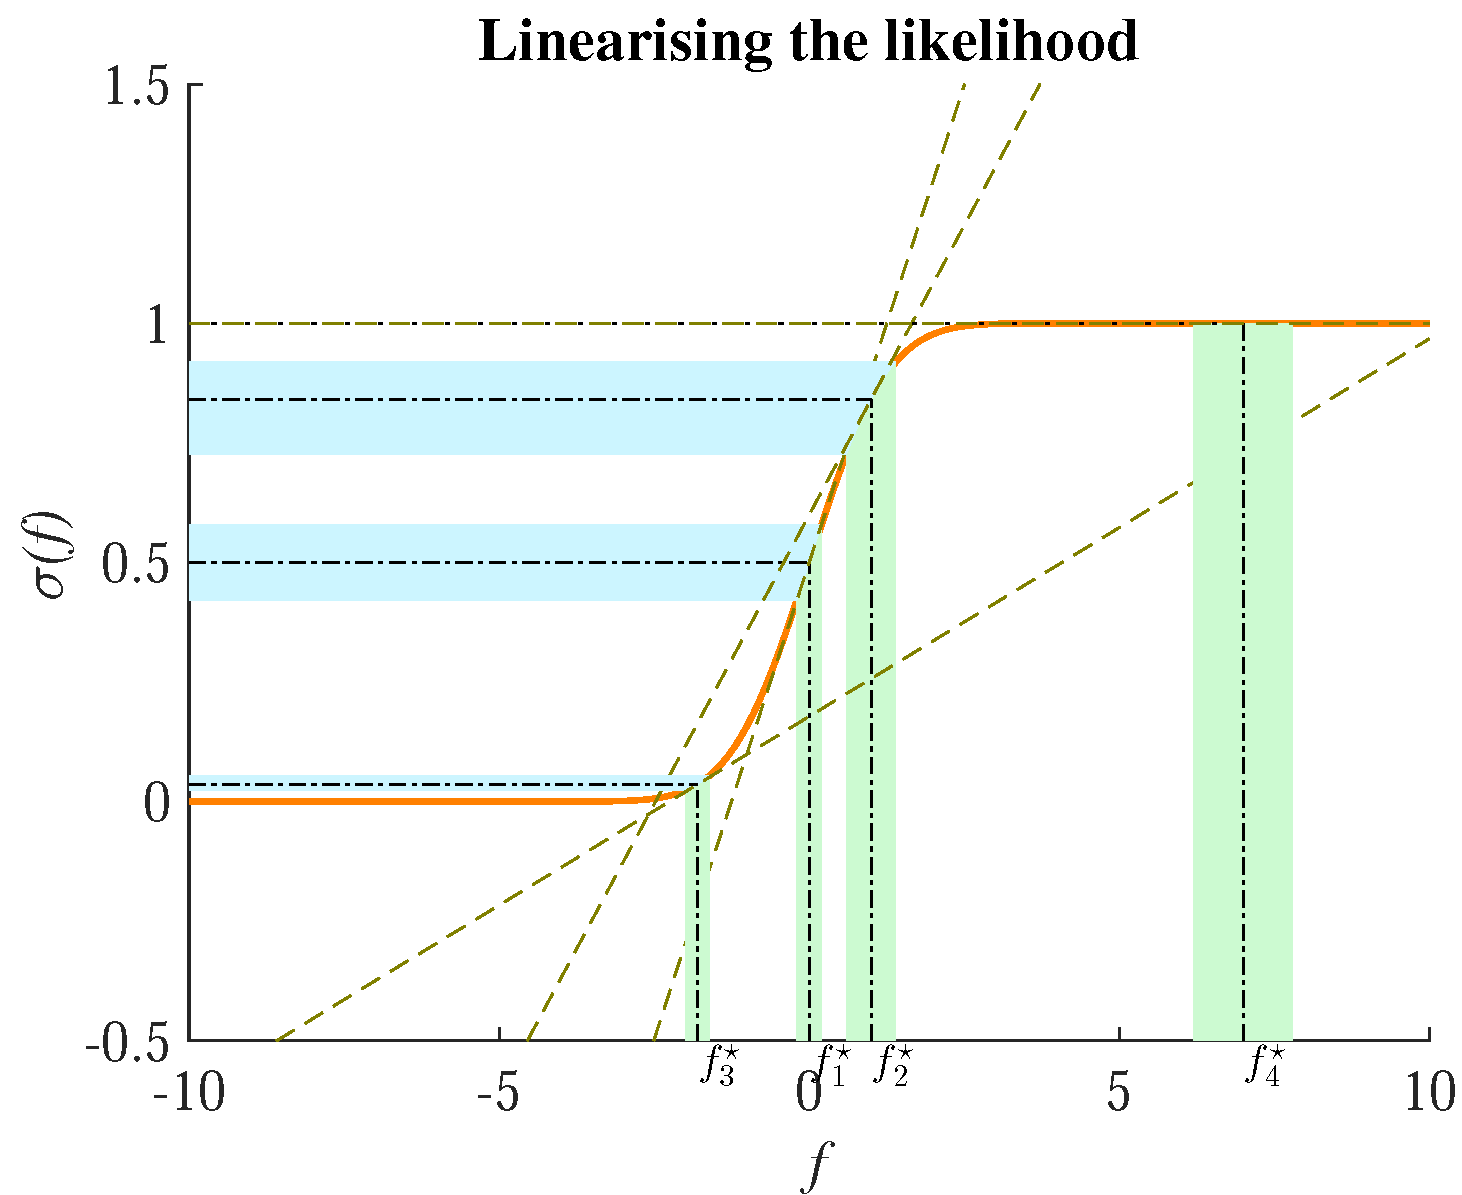
\includegraphics[width = \linewidth]{Figures/linearisation-eps-converted-to.png}
			\caption{Linearisation accuracy for a probit response: Green shade represents the latent variance while blue shade represents the predictive variance. Gold lines show local linearisation about latent expectance.}
			\label{Figure:Linearisation}
		\end{figure}
			
		As the predictive probabilities are nonlinear transformations of the Gaussian distributed latent vector, they are no longer Gaussian distributed. In order to retain analytical tractability, we propose linearising the response function about the latent expectance $\bar{f}^{\star}_{i} := \mathbb{E}[f^{\star}_{i}]$. Figure \ref{Figure:Linearisation} illustrates the linearisation accuracy for a probit response. Observe that points with latent expectance far away from zero translate to near zero predictive variance even under high latent variance. Linearisation is thus very accurate for those points. For points with latent expectances near zero, we require the latent variances to be sufficiently small for linearisation to be accurate.
		
		\subsubsection{Derivation}
		
			We proceed to derive the linearisation which also serves to construct the definition of linearised differential entropy. With first order Taylor expansion, we linearise the response about the latent mean $\bar{f}^{\star}_{i} = \mathbb{E}[f^{\star}_{i}]$ \eqref{Section:LinearisedEntropy:Equation:LinearisingSigmoid}. \begin{equation}
				\sigma(f^{\star}_{i}) \approx \sigma_{L}(f^{\star}_{i}) := \sigma(\bar{f}^{\star}_{i}) + \sigma'(\bar{f}^{\star}_{i}) (f^{\star}_{i} - \bar{f}^{\star}_{i})
			\label{Section:LinearisedEntropy:Equation:LinearisingSigmoid}
			\end{equation}
			
			The prediction probabilities are now approximated as a linear transformation $\sigma_{L}(f)$ of the latent vector, so that it is also multivariate Gaussian distributed with expectance and covariance available in analytical form \eqref{Section:LinearisedEntropy:Equation:MomentsLinearisedSigmoid}. \begin{align*}
			\numberthis \label{Section:LinearisedEntropy:Equation:MomentsLinearisedSigmoid}
					\vec{\upsigma}_{L}(\bvec{f}^{\star}) & \sim \mathcal{N}(\vec{\upmu}^{\star}_{L}, \Sigma^{\star}_{L}) \\
					({\mu^{\star}_{L}})_{i} & = \mathbb{E}[\sigma_{L}(f^{\star}_{i})] = \sigma(\bar{f}^{\star}_{i}) \\
					({\Sigma^{\star}_{L}})_{ij} & = \mathbb{C}\mathrm{ov}[\sigma_{L}(f^{\star}_{i}), \sigma_{L}(f^{\star}_{j})] = \sigma'(\bar{f}^{\star}_{i}) \sigma'(\bar{f}^{\star}_{j}) \mathbb{C}\mathrm{ov}[f^{\star}_{i}, f^{\star}_{j}]
			\end{align*}
			
			We then define the linearised differential entropy $H^{\star}_{L}$ at the query points $X^{\star}$ to be the differential entropy for which the random vector $\vec{\upsigma}_{L}(\bvec{f}^{\star})$ holds. Since $\vec{\upsigma}_{L}(\bvec{f}^{\star})$ is multivariate Gaussian distributed, $H_{L}$ exhibits a closed form \eqref{Section:LinearisedEntropy:Equation:BinaryLinearisedEntropy}. \begin{equation}
				H^{\star}_{L} := \frac{1}{2} \log\Big((2 \pi e)^{n^{\star}} \det(\Sigma^{\star}_{L})\Big)
			\label{Section:LinearisedEntropy:Equation:BinaryLinearisedEntropy}
			\end{equation}			
					
	\subsection{Multiclass Classification}
			
		For multiclass classification, linearisation is performed on the softmax function $\sigma^{m}$ which returns the corresponding predictive class probability $\vec{\uppi}^{m}$ for class $m \in \{1, 2, \dots, c\}$ \eqref{Section:LinearisedEntropy:Equation:Softmax} \cite{GaussianProcessForMachineLearning}. For notational clarity we move the query star ($^\star$) to the left and use the superscript $m$ to index the classes. The latent vector $\bvec{f}_{i} := \{f^{m}_{i}\}_{m \in \{1, 2, \dots, c\}}$ represents the collection of $c$ latent values across classes at the query point $i$, and is distinct from $\bvec{f}^{m} := \{f^{m}_{i}\}_{i \in \{1, 2, \dots, n^{\star}\}}$ which represents the collection of $n^{\star}$ latent values across query points for class $m$. \begin{equation}
			^{\star}\pi^{m}_{i} = \sigma^{m}(^{\star}\bvec{f}_{i}) := \frac{\exp(^{\star}f^{m}_{i})}{\sum_{l = 1}^{c} \exp(^{\star}f^{l}_{i})} \qquad m \in \{1, 2, \dots, c\}
		\label{Section:LinearisedEntropy:Equation:Softmax}
		\end{equation}
		
		In this derivation, we focus on the case of OVA, or one versus all, multiclass classification, where each class is trained against all other classes independently with a binary classifier. For $c$ classes, $c$ binary classifiers are trained independently and also performs inference independently. The normalisation is then inherently captured in the softmax \eqref{Section:LinearisedEntropy:Equation:Softmax}. This approach avoids the Monte Carlo sampling step in the inference stage of a typical GP multiclass classifier under Laplace Approximation \cite{GaussianProcessForMachineLearning}, and is thus faster in computational time. Furthermore, because each classifier is trained independently, both the learning stage and the inference stage can be performed in parallel, further speeding up the process in a way that was not available under the original scheme. This is important later in under a receding horizon formulation, where the inference stage is included in the objective function of an optimiser such that repeated evaluations would benefit dramatically from shorter inference time.
		
		\subsubsection{Derivation}
		
			Similar to the binary case, to linearise we first find the gradient of each of the $c$ softmax functions \eqref{Section:LinearisedEntropy:Equation:SoftmaxGradient}. For notational simplicity, the query stars ($^{\star}$) are omitted in this derivation except for $n^{\star}$.
			
			\begin{equation}
				\frac{\partial \sigma^{m}}{\partial f^{k}_{i}}(\bvec{f}_{i}) =
				\begin{cases} 
					- \frac{\exp(f^{m}_{i}) \exp(f^{k}_{i})}{\sum_{l = 1}^{c} \exp(f^{l}_{i})} & \text{for } k \neq m  \\
					- \frac{\exp(f^{m}_{i})^{2}}{\big(\sum_{l = 1}^{c} \exp(f^{l}_{i})\big)^{2}} + \frac{\exp(f^{m}_{i})}{\sum_{l = 1}^{c} \exp(f^{l}_{i})}& \text{for } k = m
				\end{cases}
			\label{Section:LinearisedEntropy:Equation:SoftmaxGradient}
			\end{equation}			
		
			The numerators are explicitly left in the form of products of exponentiation instead of exponentiation of sums to reflect ways to cache quantities during computation. 
			
			Hence, for each class $m$ at query point $i$ we compute a softmax gradient vector \eqref{Section:LinearisedEntropy:Equation:SoftmaxGradientVector}.
			
			\begin{equation}
				\frac{\partial \sigma^{m}}{\partial \bvec{f}_{i}}(\bvec{f}_{i}) := \begin{bmatrix} \frac{\partial \sigma^{m}}{\partial f^{1}_{i}}(\bvec{f}_{i}) & \frac{\partial \sigma^{m}}{\partial f^{2}_{i}}(\bvec{f}_{i}) & \dots & \frac{\partial \sigma^{m}}{\partial f^{c}_{i}}(\bvec{f}_{i}) \end{bmatrix}^{T}
			\label{Section:LinearisedEntropy:Equation:SoftmaxGradientVector}
			\end{equation}
			
			The linearisation is again performed on the mean latent predictions $\bar{\bvec{f}}_{i} = \mathbb{E}[\bvec{f}_{i}]$ so that the we can approximate the softmax $\sigma^{m}(\bvec{f}_{i})$ with the linearised softmax $\sigma^{m}_{L}(\bvec{f}_{i})$ \eqref{Section:LinearisedEntropy:Equation:LinearisedSoftmax} in an analogous form as \eqref{Section:LinearisedEntropy:Equation:LinearisingSigmoid}.
			
			\begin{equation}
				\begin{aligned}
					\sigma^{m}(\bvec{f}_{i}) \approx \sigma^{m}_{L}(\bvec{f}_{i}) & := \sigma^{m}(\bar{\bvec{f}}_{i}) + \left. \frac{\partial \sigma^{m}}{\partial \bvec{f}_{i}} \right|^{T}_{\bvec{f}_{i} = \bar{\bvec{f}}_{i}} (\bvec{f}_{i} - \bar{\bvec{f}}_{i}) \\
					& = \bvec{c}^{m}_{i} + (\bvec{g}^{m}_{i})^{T} (\bvec{f}_{i} - \bar{\bvec{f}}_{i})
				\end{aligned}
			\label{Section:LinearisedEntropy:Equation:LinearisedSoftmax}
			\end{equation}
			
			where we have notated the constants $\bvec{c}^{m}_{i} := \sigma^{m}(\bar{\bvec{f}}_{i})$ and $\bvec{g}^{m}_{i} := \frac{\partial \sigma^{m}}{\partial \bvec{f}_{i}}(\bar{\bvec{f}}_{i})$.
			
			To determine the distribution of the vector of softmax values across query points, we first define the following \eqref{Section:LinearisedEntropy:Equation:Definitions}.
			
			\begin{equation}
				\begin{aligned}
					F &:= \{f^{m}_{i}\}_{m \in \{1, 2, \dots, c\}, i \in \{1, 2, \dots, n^{\star}\}} \in \mathbb{R}^{c \times n^{\star}} \\
					\vec{\upsigma}^{m}_{L}(F) &:= \begin{bmatrix} \sigma^{m}_{L}(\bvec{f}_{1}) & \sigma^{m}_{L}(\bvec{f}_{2}) & \dots & \sigma^{m}_{L}(\bvec{f}_{n}) \end{bmatrix}^{T}
				\end{aligned}
			\label{Section:LinearisedEntropy:Equation:Definitions}
			\end{equation}
						
			We can now compute the covariance of the linearised sigmoid of a particular class $m$ between two query points $i$ and $j$, as well as the expectance at a particular query point $i$ \eqref{Section:LinearisedEntropy:Equation:MomentsLinearisedSoftmax}.
			
			\begin{align*}
			\numberthis \label{Section:LinearisedEntropy:Equation:MomentsLinearisedSoftmax}
					\vec{\upsigma}^{m}_{L}(F) & \sim \mathcal{N}(\vec{\upmu}^{m}_{L}, \Sigma^{m}_{L}) \\
					(\mu^{m}_{L})_{i} & = \mathbb{E}[\sigma^{m}_{L}(\bvec{f}_{i})] =  \sigma^{m}(\bar{\bvec{f}}_{i}) \\
					(\Sigma^{m}_{L})_{ij} & = \mathbb{C}\mathrm{ov}[\sigma^{m}_{L}(\bvec{f}_{i}), \sigma^{m}_{L}(\bvec{f}_{i})] \\
					& = \mathbb{C}\mathrm{ov}[(\bvec{g}^{m}_{i})^{T} \bvec{f}_{i}, (\bvec{g}^{m}_{j})^{T} \bvec{f}_{j}] \\
					& = \sum_{k = 1}^{c} (g^{m}_{i})^{k} (g^{m}_{j})^{k} \mathbb{C}\mathrm{ov}[f^{k}_{i}, f^{k}_{j}]
			\end{align*}
						
			where $(g^{m}_{i})^{k}$ denotes the $k^{\text{th}}$ element of $\bvec{g}^{m}_{i}$. The last equality arises as a result of employing OVA multiclass classification, where latent values of class $i$ and class $j$ are conditionally independent given training observations.
			
			Finally, we define the linearised entropy of the OVA multiclass Gaussian process classifier as follows \eqref{Section:LinearisedEntropy:Equation:MulticlassLinearisedEntropy}.
			
			\begin{equation}
				H_{L} := \frac{1}{2} \log\Bigg((2 \pi e)^{n^{\star}} \det\bigg(\sum_{m = 1}^{c} \Sigma^{m}_{L}\bigg)\Bigg)
			\label{Section:LinearisedEntropy:Equation:MulticlassLinearisedEntropy}
			\end{equation}			
	
	\subsection{Interpretation of Linearised Differential Entropy}
	
		It is worthwhile to remember that linearised differential entropy is not an approximation to the usual prediction information entropy - the former is a differential entropy on a multivariate Gaussian distribution and the latter is an information entropy on the distribution of discrete class predictions combinations, which is a multivariate multinomial distribution. They have different interpretations and both can have advantageous properties under different scenarios. We propose using linearised differential entropy as an alternative acquisition function for informative path planning which can be more beneficial under specific exploration purposes.
		
		Specifically, while the prediction information entropy (PIE) represents the confidence in the model, the linearised differential entropy (LDE) represents the the separability of classes in the feature space. In fact, LDE quantifies the ambiguity of the predictive probabilities. In particular, it is possible for GP multiclass classifiers to conclude low predictive variance even under uncertain predictive probabilities. In this case, the LDE would be high while the PIE would be low at such locations, indicating that the model is confident about its inability to separate classes \cite{AsherBender}. Similar to the bias-variance trade-off, such a situation indicate high bias, and is distinct from a model that is unconfident about its ability to separate classes, which would correspond to high variance. This demonstrates that PIE and LDE are two complementary measures of entropy that can assist each other in identifying both places of high bias and high variance.
		
		In the case of informative path planning, a measure of mutual information is required. While the formulation of LDE readily incorporates joint distributions \eqref{Section:LinearisedEntropy:Equation:MulticlassLinearisedEntropy}, to obtain the joint PIE one would need to perform estimations from techniques such as Monte Carlo sampling. We refer to the latter as Monte Carlo estimated Joint Information Entropy (MCJIE).
		
		Here we compare linearised differential entropy and the usual prediction information entropy of a Gaussian process classifier. For visualisation purposes, only the marginalised entropies across the feature space are shown. We show examples where abundant information is available, so that the difference in the properties in the two measures can be emphasized. 
		
		Figure \ref{Figure:Results:BinaryLinearisedEntropy} shows a simple binary classification problem with abundant data on features $x_{1}$ and $x_{2}$, allowing a misclassification rate of 2.155\%. The classifier is trained with an axis aligned Gaussian kernel with a probit response under Laplace approximation. 

		\begin{figure}[t]
		\centering
			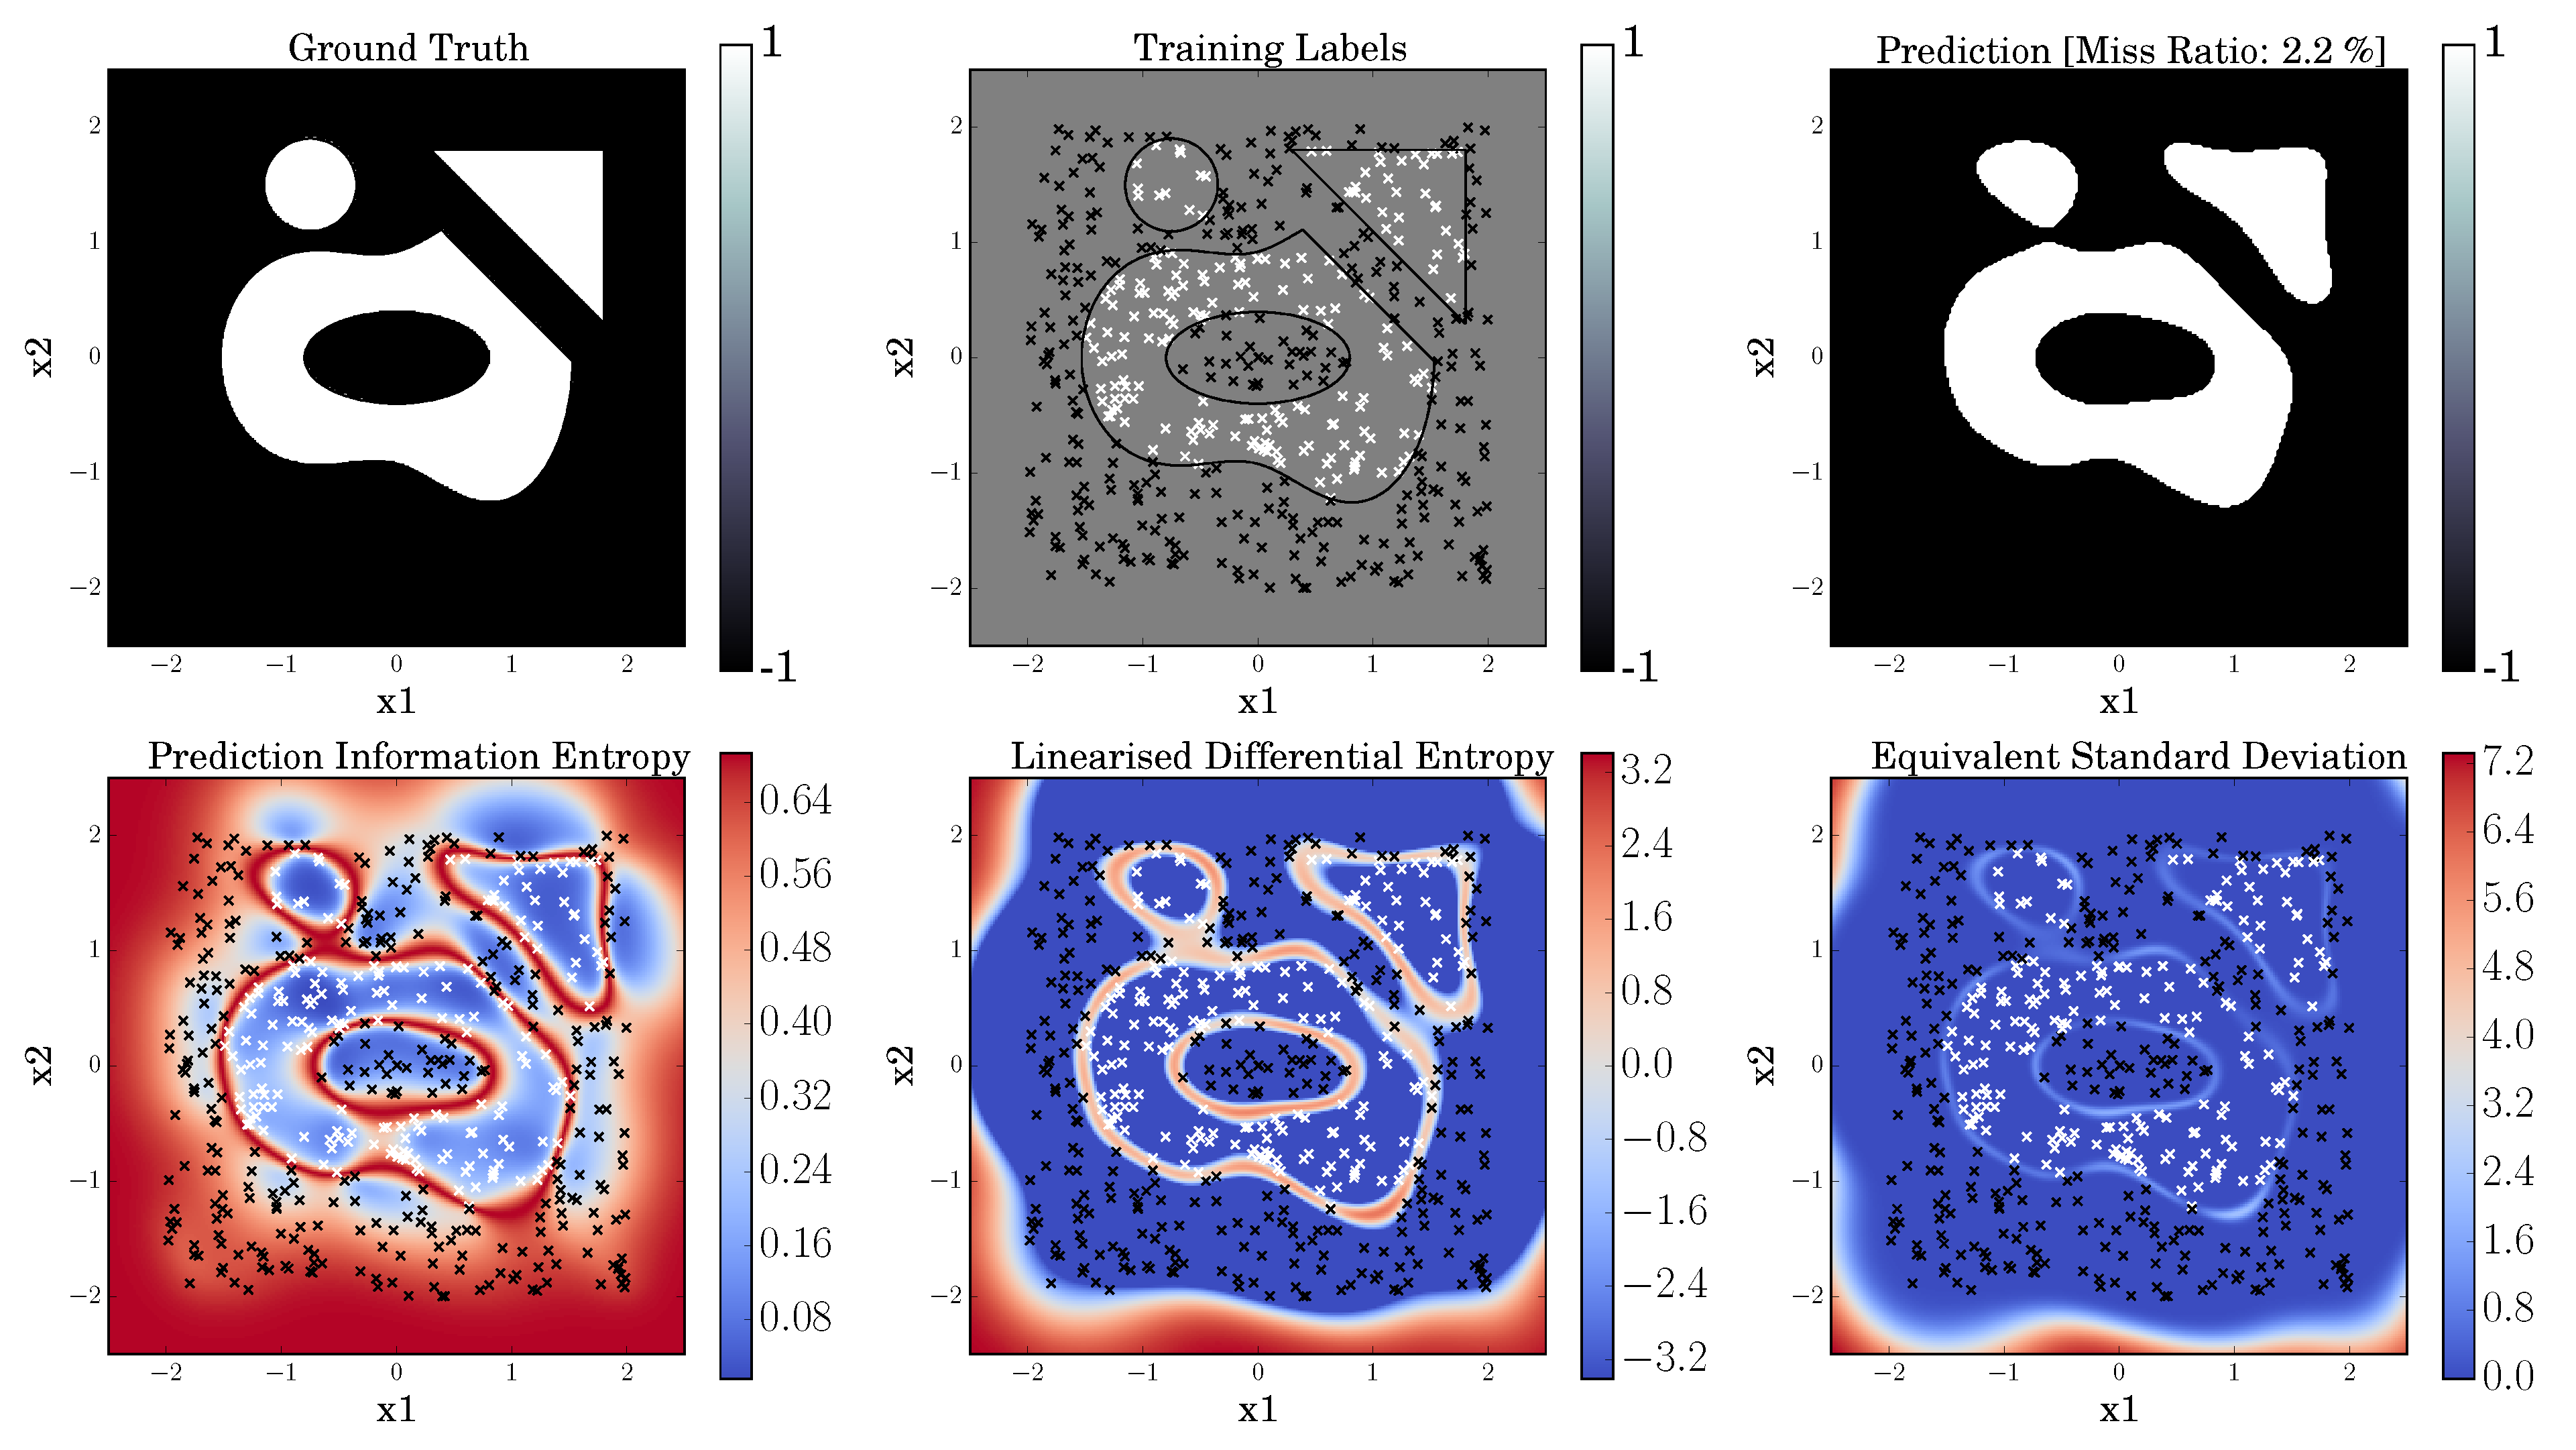
\includegraphics[width = \linewidth]{Figures/binary-eps-converted-to.png}
		\caption{GP binary classifier: prediction information entropy and linearised differential entropy under abundant data}
		\label{Figure:Results:BinaryLinearisedEntropy}
		\end{figure}
		
		In this example, there are no training points around the edges shown. As a result, the GP classifier learns a slightly lower signal to noise ratio in the latent function, and bounces back to its latent GP prior for which it remains uncertain regarding class label assignments. The prediction information entropy reflects this change more rapidly, so that it is high both at the decision boundaries and wherever observations are lacking. If the acquisition function for informative exploration is a function of the prediction information entropy, the vehicle would be suggested to explore both places with lacking observations and the decision boundaries. 
		
		On the other hand, linearised differential entropy focuses on the decision boundary as it is constructed to be only high when the latent function is near zero (figure \ref{Figure:Linearisation}). We can see in Figure \ref{Figure:Results:BinaryLinearisedEntropy} that the linearised differential entropy emphasizes on where the latent expectance is close to zero, and filters out the rest. If the linearised differential entropy is used as the acquisition function, the vehicle would focus on the decision boundaries within the feature space. Notice that regions far away from observations in the feature space are also assigned with high linearised differential entropy, as the latent function bounces back to its prior, so that the vehicle would explore those parts of the feature space if necessary.
		
%		Intuitively, under abundant data, we would like the classifier to only indicate high entropies at decision boundaries. In Figure \ref{Figure:Results:BinaryLinearisedEntropy}, we see that the prediction information entropy is indeed near its maximum at the predict decision boundaries. As an artefact of the Laplace approximation, however, it is also quite high around the edges where the classifier has learned a slightly lower signal to noise ratio. As there are no data points around the edges, the GP classifier learns a latent function that bounces back to its latent GP prior for which it remains uncertain regarding the class labels. 
		
%		This suggests that if the prediction information entropy is used as the acquisition function for path planning, the vehicle would be suggested to spent some time travelling around the region of interest, collecting data it is already expecting. The prediction entropy is high at both predicted decision boundaries and also places with lower relative data density compared. 
%		
%		This leads to the classic exploration-exploitation dilemma most machine learning algorithms face. It is possible that there exists decision boundaries yet to be detected at regions of lower relative data density. Is it worth it for the vehicle to explore and discover such regions, or exploit the currently known boundaries and map it better? In most exploration applications, the priority is to map the region of interest as accurately and fast as possible in order to reduce time and cost. While it is possible that there exists undiscovered decision boundaries at regions of lower relative data density, it is undesirable under cost constraints that this possibility is weighed heavily by the vehicle even under abundant data.
		
		This demonstrates the advantage of linearised differential entropy. We can see in Figure \ref{Figure:Results:BinaryLinearisedEntropy} that the linearised differential entropy is only high at the predicted decision boundaries. Note that the colour scale has been centred around zero differential entropy. Under such an acquisition function, the vehicle would focus strictly on the mapping the predicted decision boundaries better.
		
		Figure \ref{Figure:Results:MulticlassLinearisedEntropy} shows a similar scenario with a multi-class scenario with 4 labels. The same behaviour as the binary case is observed, where the linearised differential entropy approach pushes down the entropy level of all regions except the predicted decision boundaries.
	
		\begin{figure}[t]
		\centering
			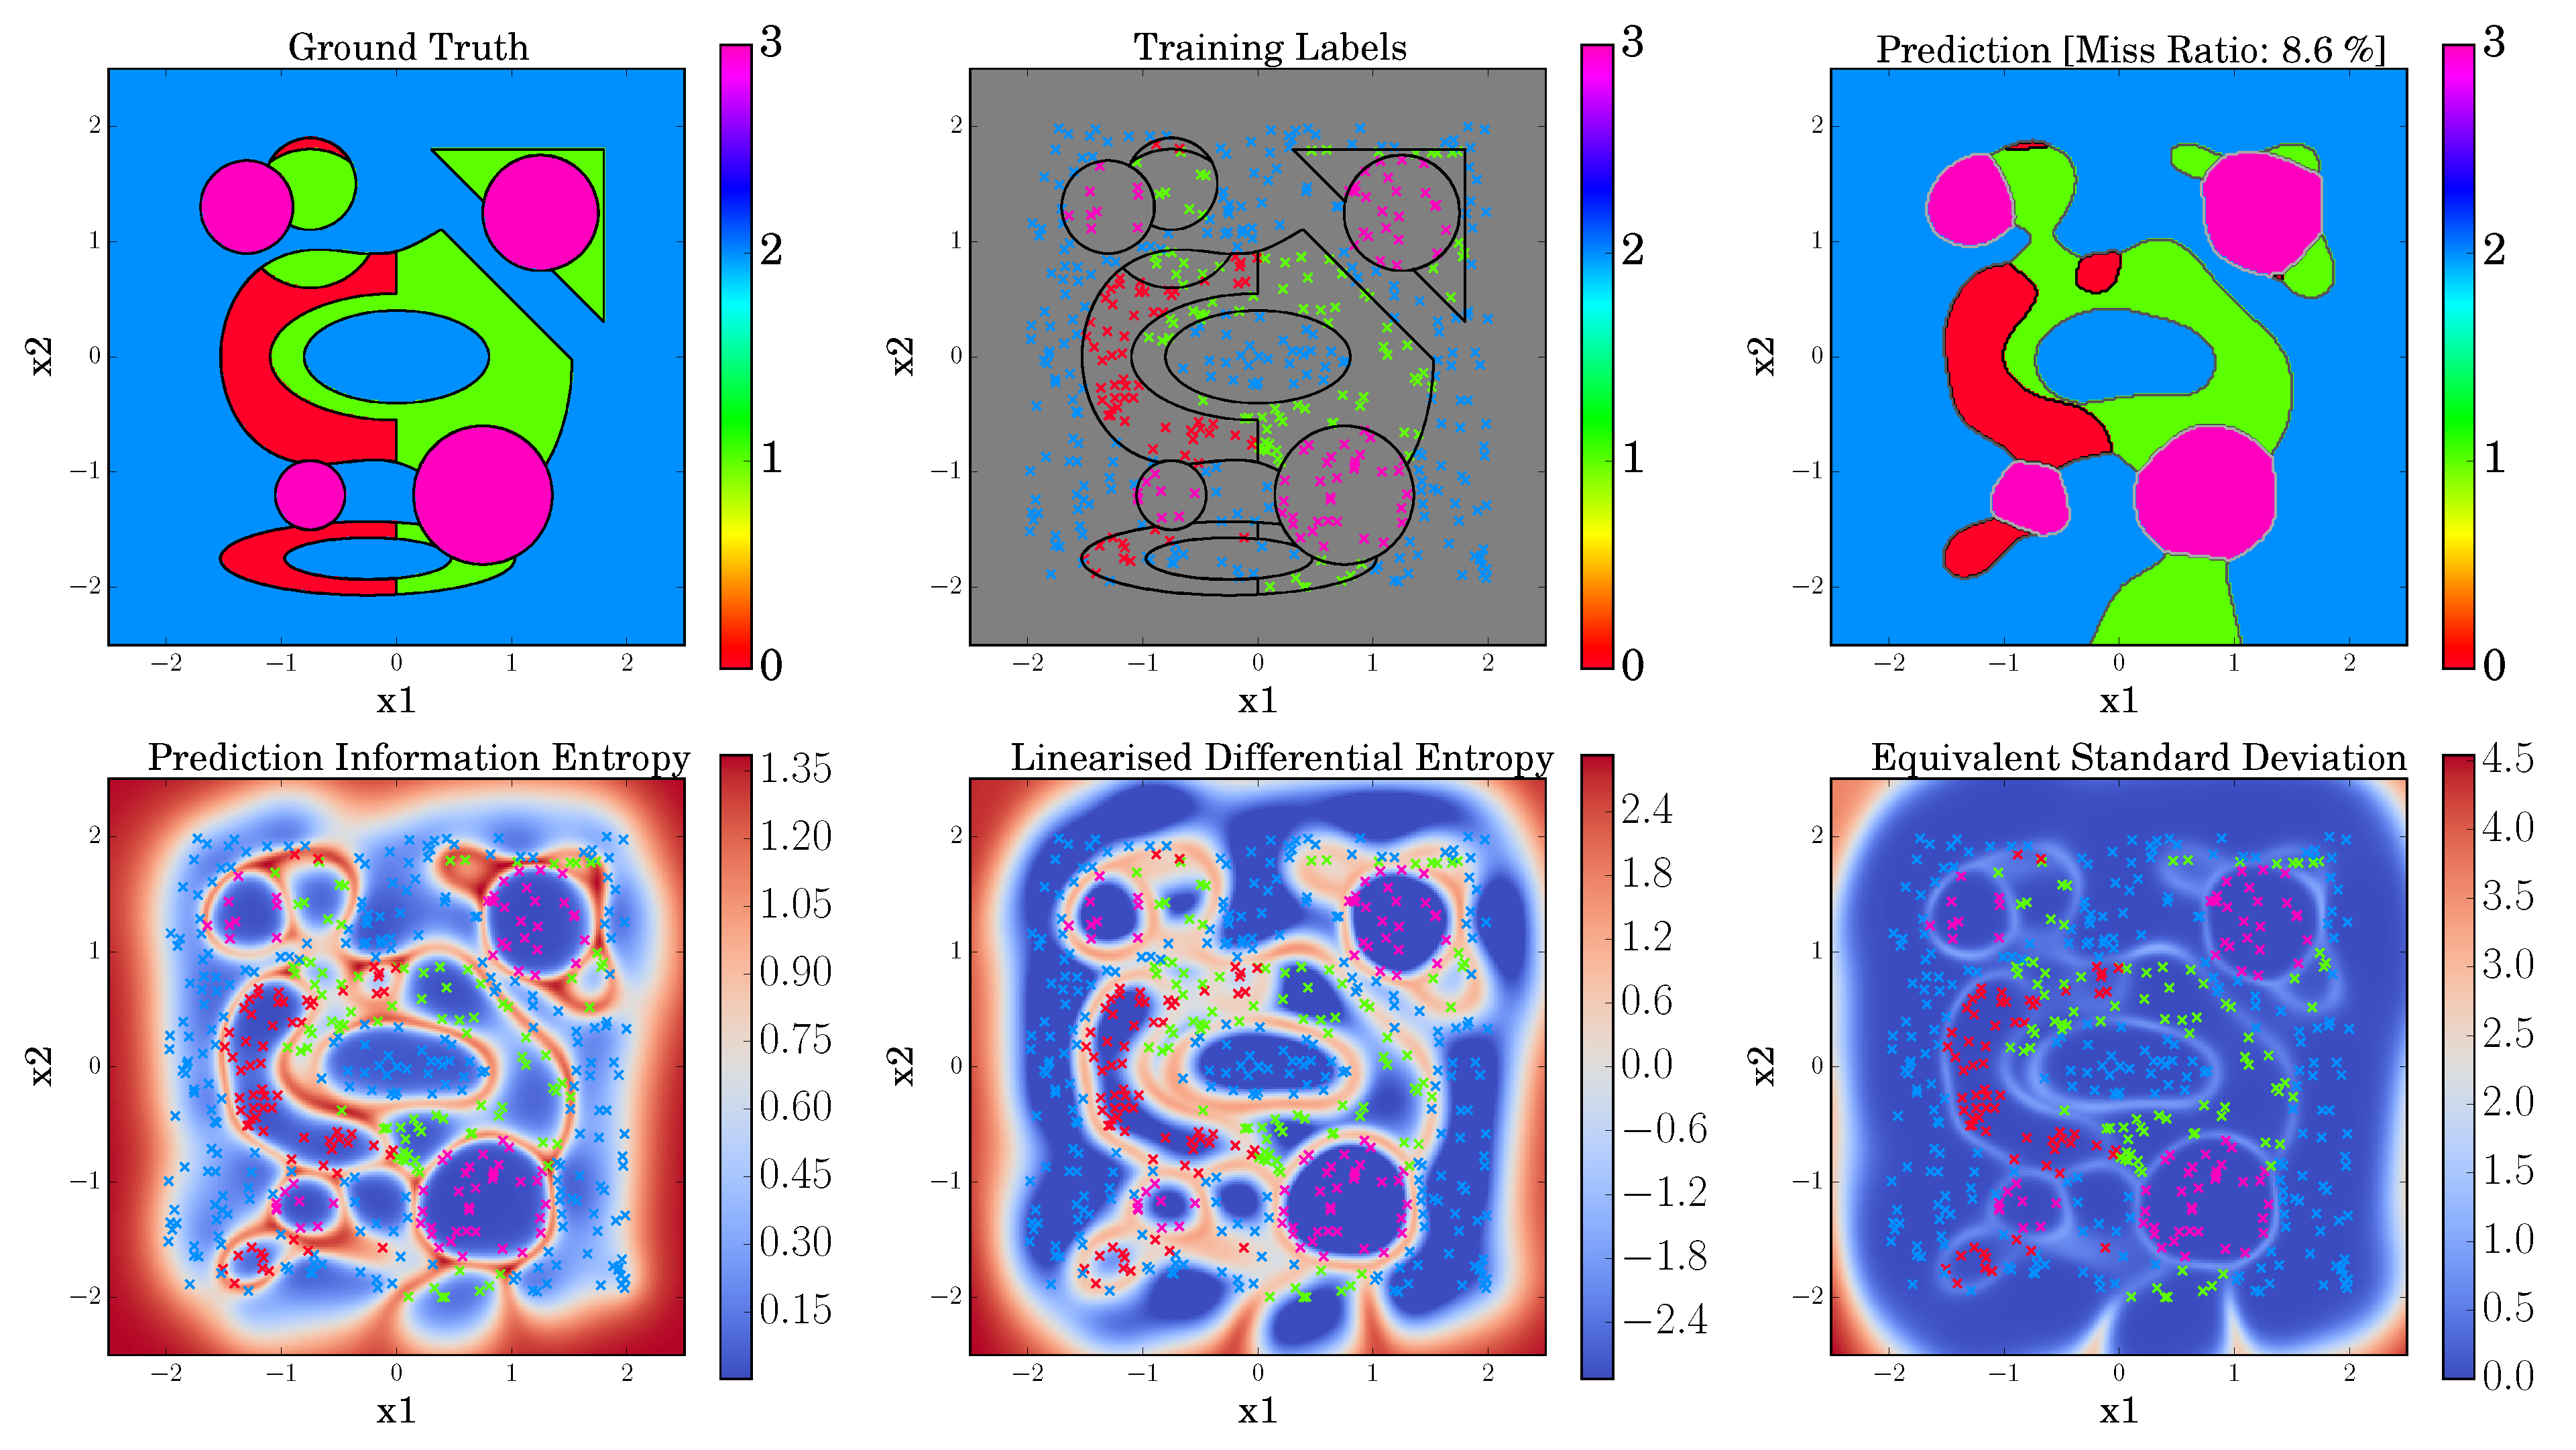
\includegraphics[width = \linewidth]{Figures/multiclass-eps-converted-to.png}
		\caption{GP multiclass classifier: prediction information entropy and linearised differential entropy under abundant data}
		\label{Figure:Results:MulticlassLinearisedEntropy}
		\end{figure}
			
%		In the case of a feature space that does not contain the spatial coordinates for which path planning in based on, the MCJIE method may spent a lot of time in a single region where it is locally rich in span of a subspace of the feature space. However, this is suboptimal as this means it is giving up on trying to go for other regions that may have an even richer span of the feature space. The linearised differential entropy method focuses its efforts (prioritises) the decision boundaries in the feature space at the expense of overlooking regions with less observations. This leads to smoother paths as it will look at all elements of the feature space. As long as one of the features is spatially correlated (depth in our case), this will lead to smoother paths.
		
\section{Receding Horizon Approach to Informative Path Planning}
\label{Section:RecedingHorizonFormulation}

	In this section we present a receding horizon approach to the informative path-planning problem. Specifically, we use the linearised differential entropy derived earlier as the acquisition function. We motivate the use of the approach and discuss its structure.
	
	The receding horizon approach is inspired by the philosophy of model predictive control (MPC) in control theory, for which a continuous problem is discretised such that an optimal control problem is transcribed into a static optimisation problem at each time step. Similar to MPC, while receding horizon methods are almost always suboptimal, it provides a computationally tractable approach that is rather stable in performance. Furthermore, a receding horizon approach avoids a myopic and greedy approach to informative path planning. Myopic approaches often result in the vehicle fixating on a region with local maximum entropy due to its inability to sacrifice immediate rewards for future rewards in a faraway region. Lastly, a receding horizon approach is simple to implement and sufficient for most missions for which strict optimality is not necessary.
	
%		Informative path planning is a highly dynamical process in which the observations the vehicle decides to take can significantly impact the belief space of the vehicle and hence alter its action. As a result, Gaussian processes are often used for modeling the environment for which path planning is to be performed. The tractability of Gaussian processes regression allows sophisticated methods for informative path planning, such as  performing sequential Bayesian optimisation to achieve informative path planning over continuous domains \cite{Roman:SequentialBayesianOptimisation}. One desired property we would like to achieve with an informative path-planning problem is that the search is non-myopic. When the objective is to collect data on a particular spatial phenomenon, Gaussian process regression can be used as the model under which strong theoretical performance guarantees can be made \cite{Meliou:2007:NIP:1619645.1619742}. However, in the case where the objective is to collect data in the form of discrete labels, a Gaussian process classifier is used instead for modeling the phenomenon. As discussed earlier, the joint entropy from a Gaussian process classifier is not available in closed form. Instead, another measure of joint entropy was developed in the previous section which demonstrated desired properties for informative exploration. To take advantage of the tractability of linearised differential entropy over finite collections of query points, we discretise the spatial domain and select paths composed of finitely many query points. The acquisition criterion is then set to be the linearised differential entropy of the query points that compose the path.

	\begin{figure*}[!htbp]
	\centering
		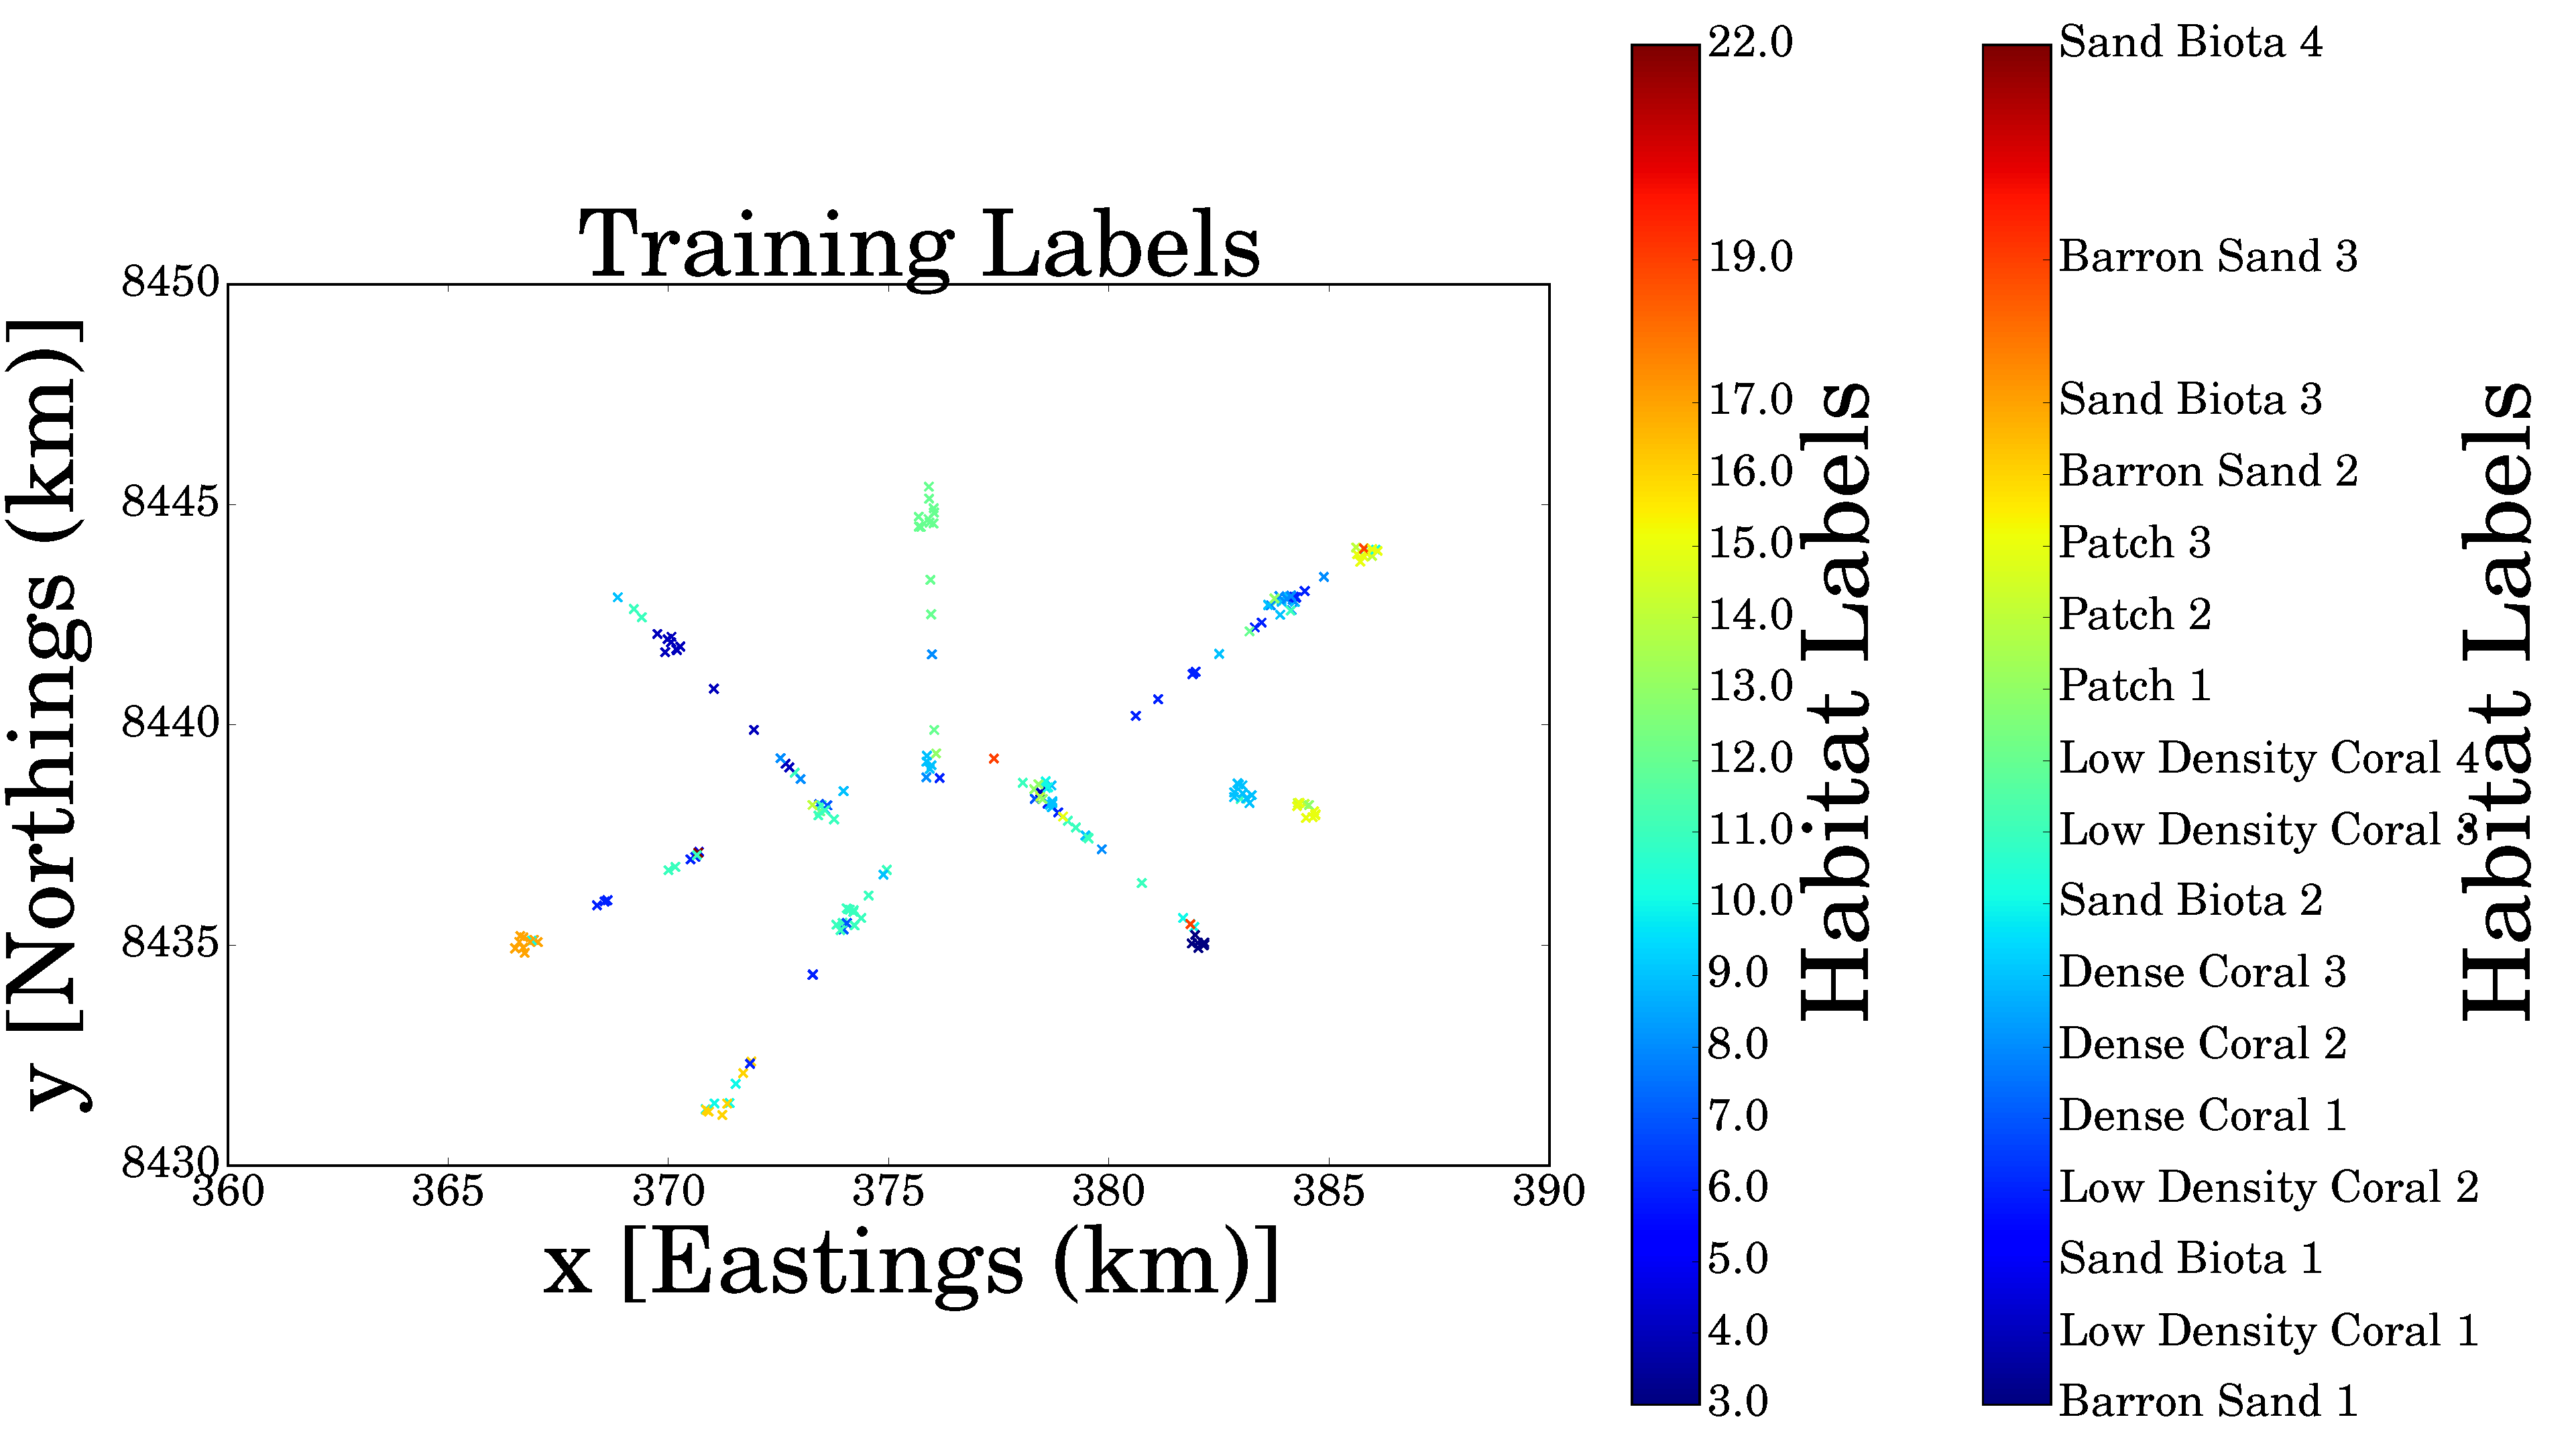
\includegraphics[width = 0.32\linewidth]{Figures/scott_reef_modeling/Figure1-eps-converted-to.png}
		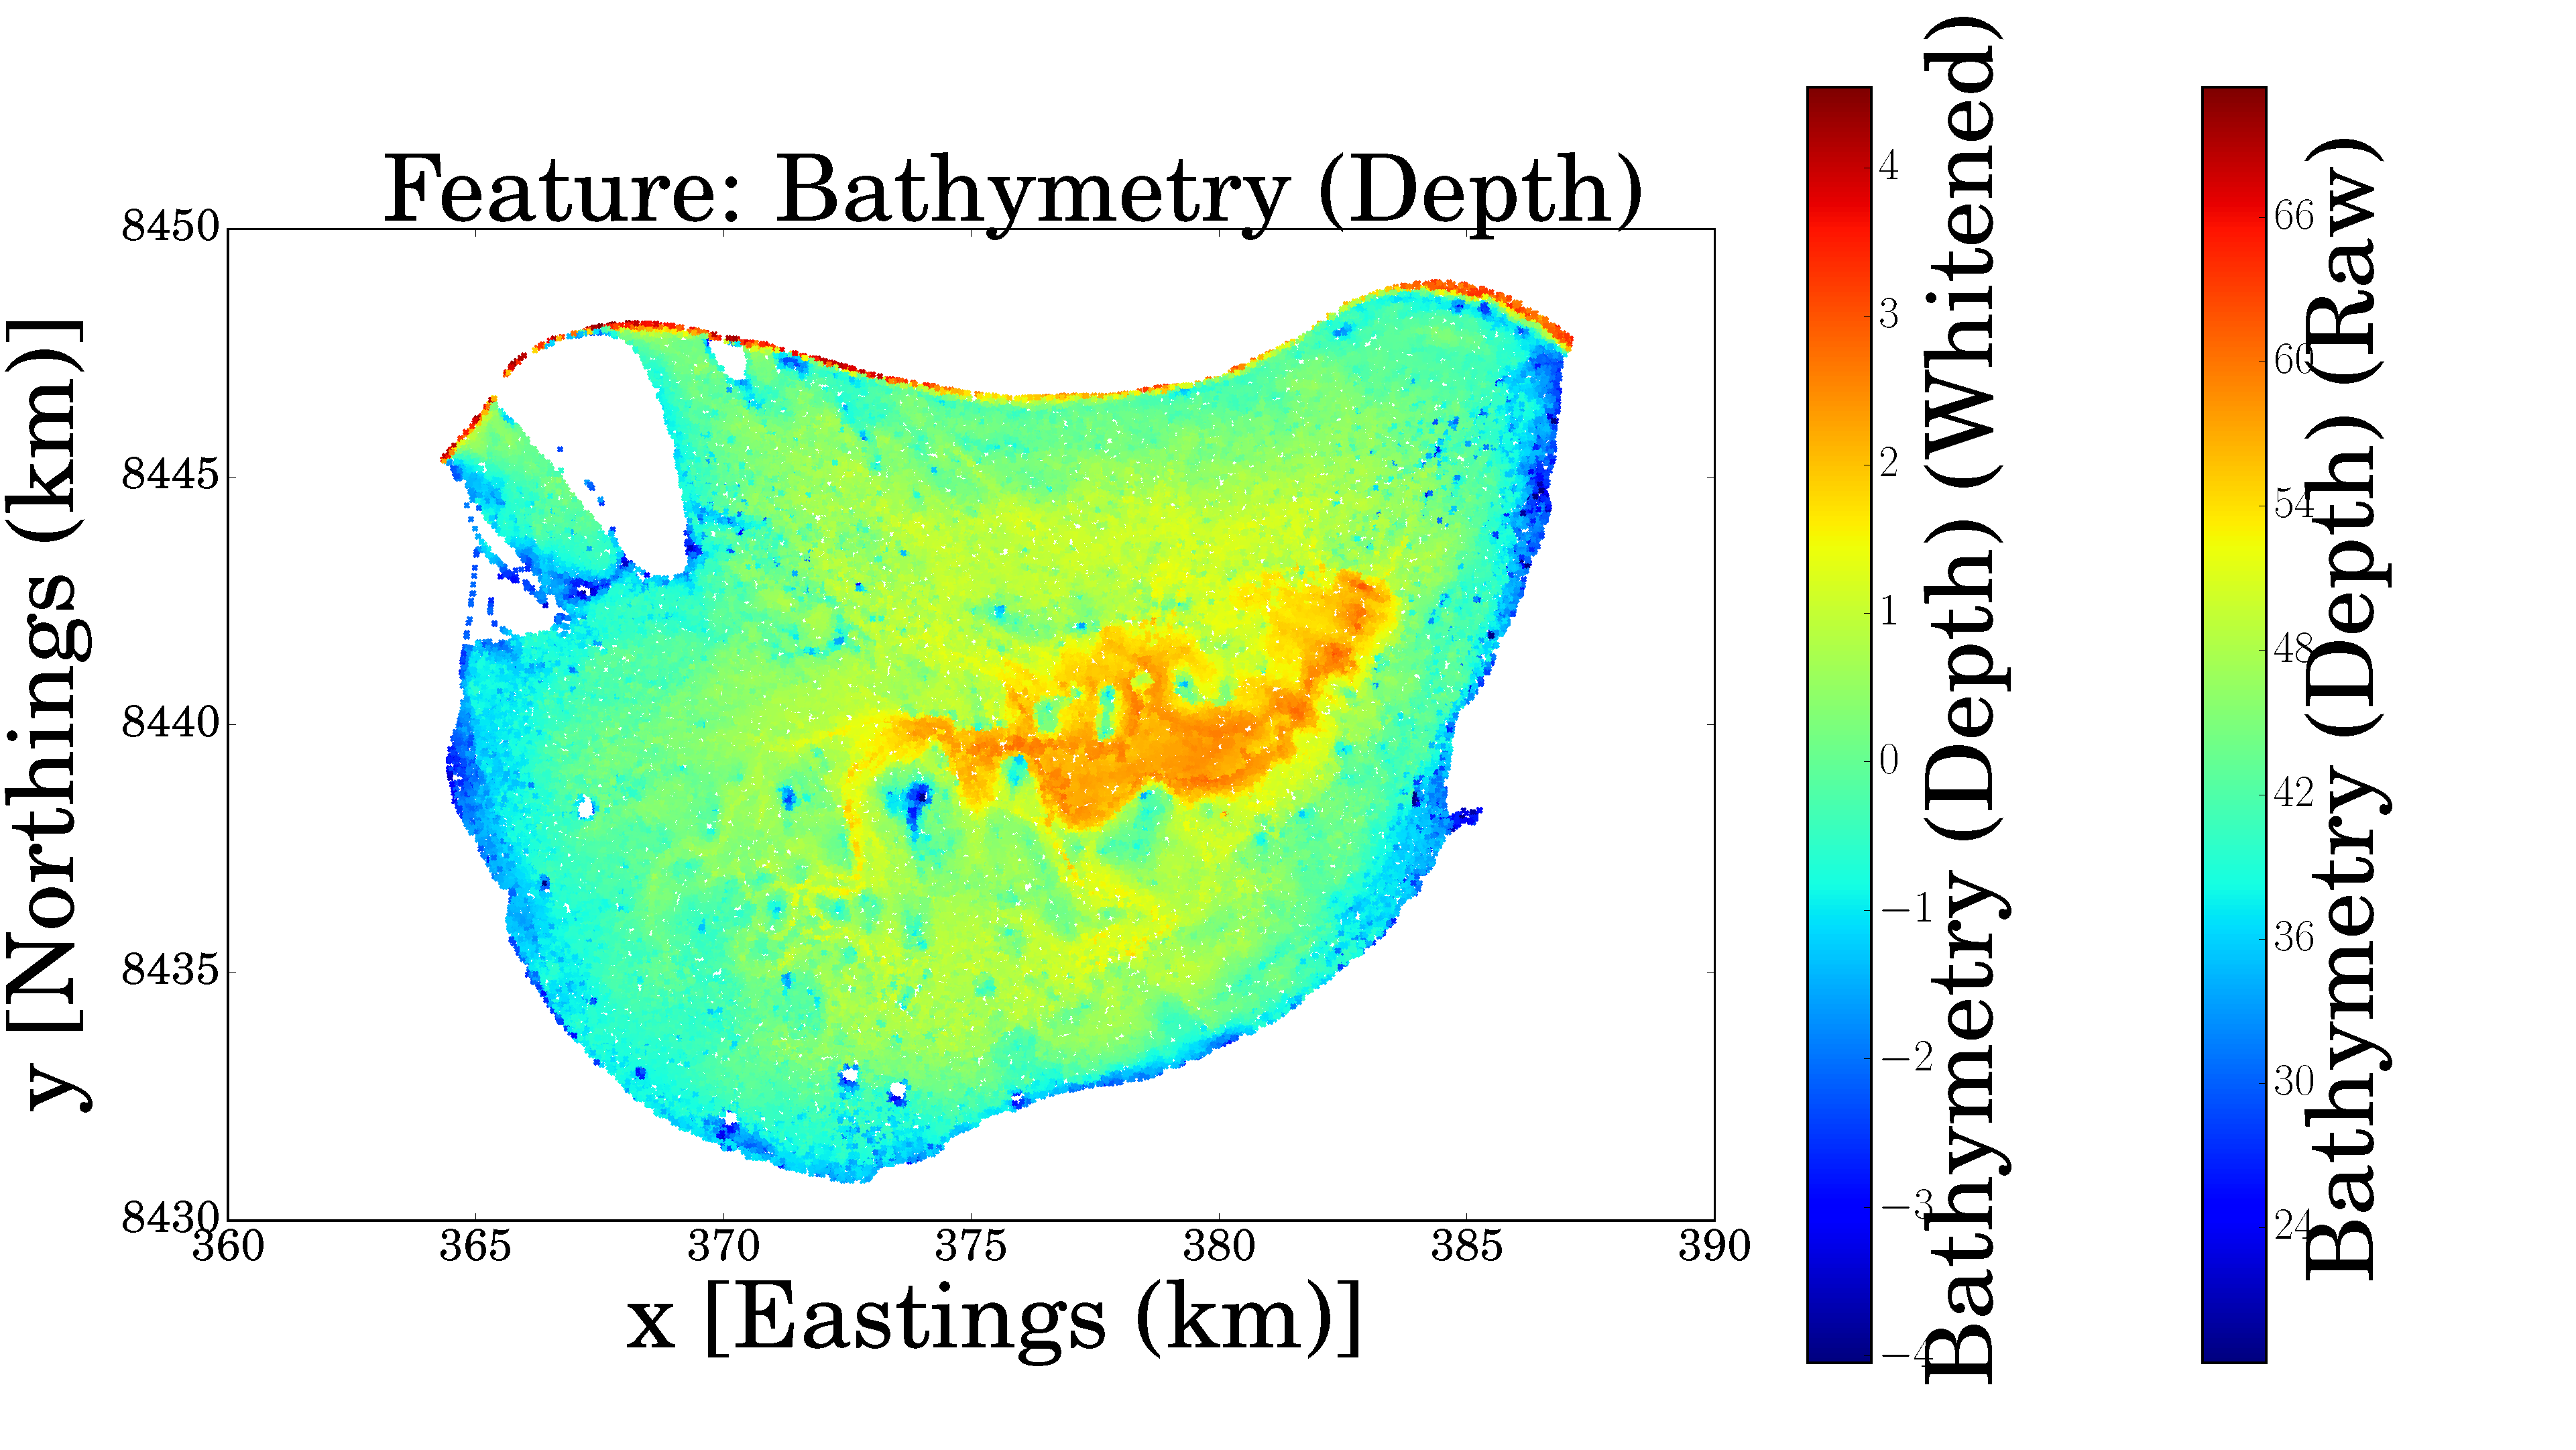
\includegraphics[width = 0.32\linewidth]{Figures/scott_reef_modeling/Figure2-eps-converted-to.png}
		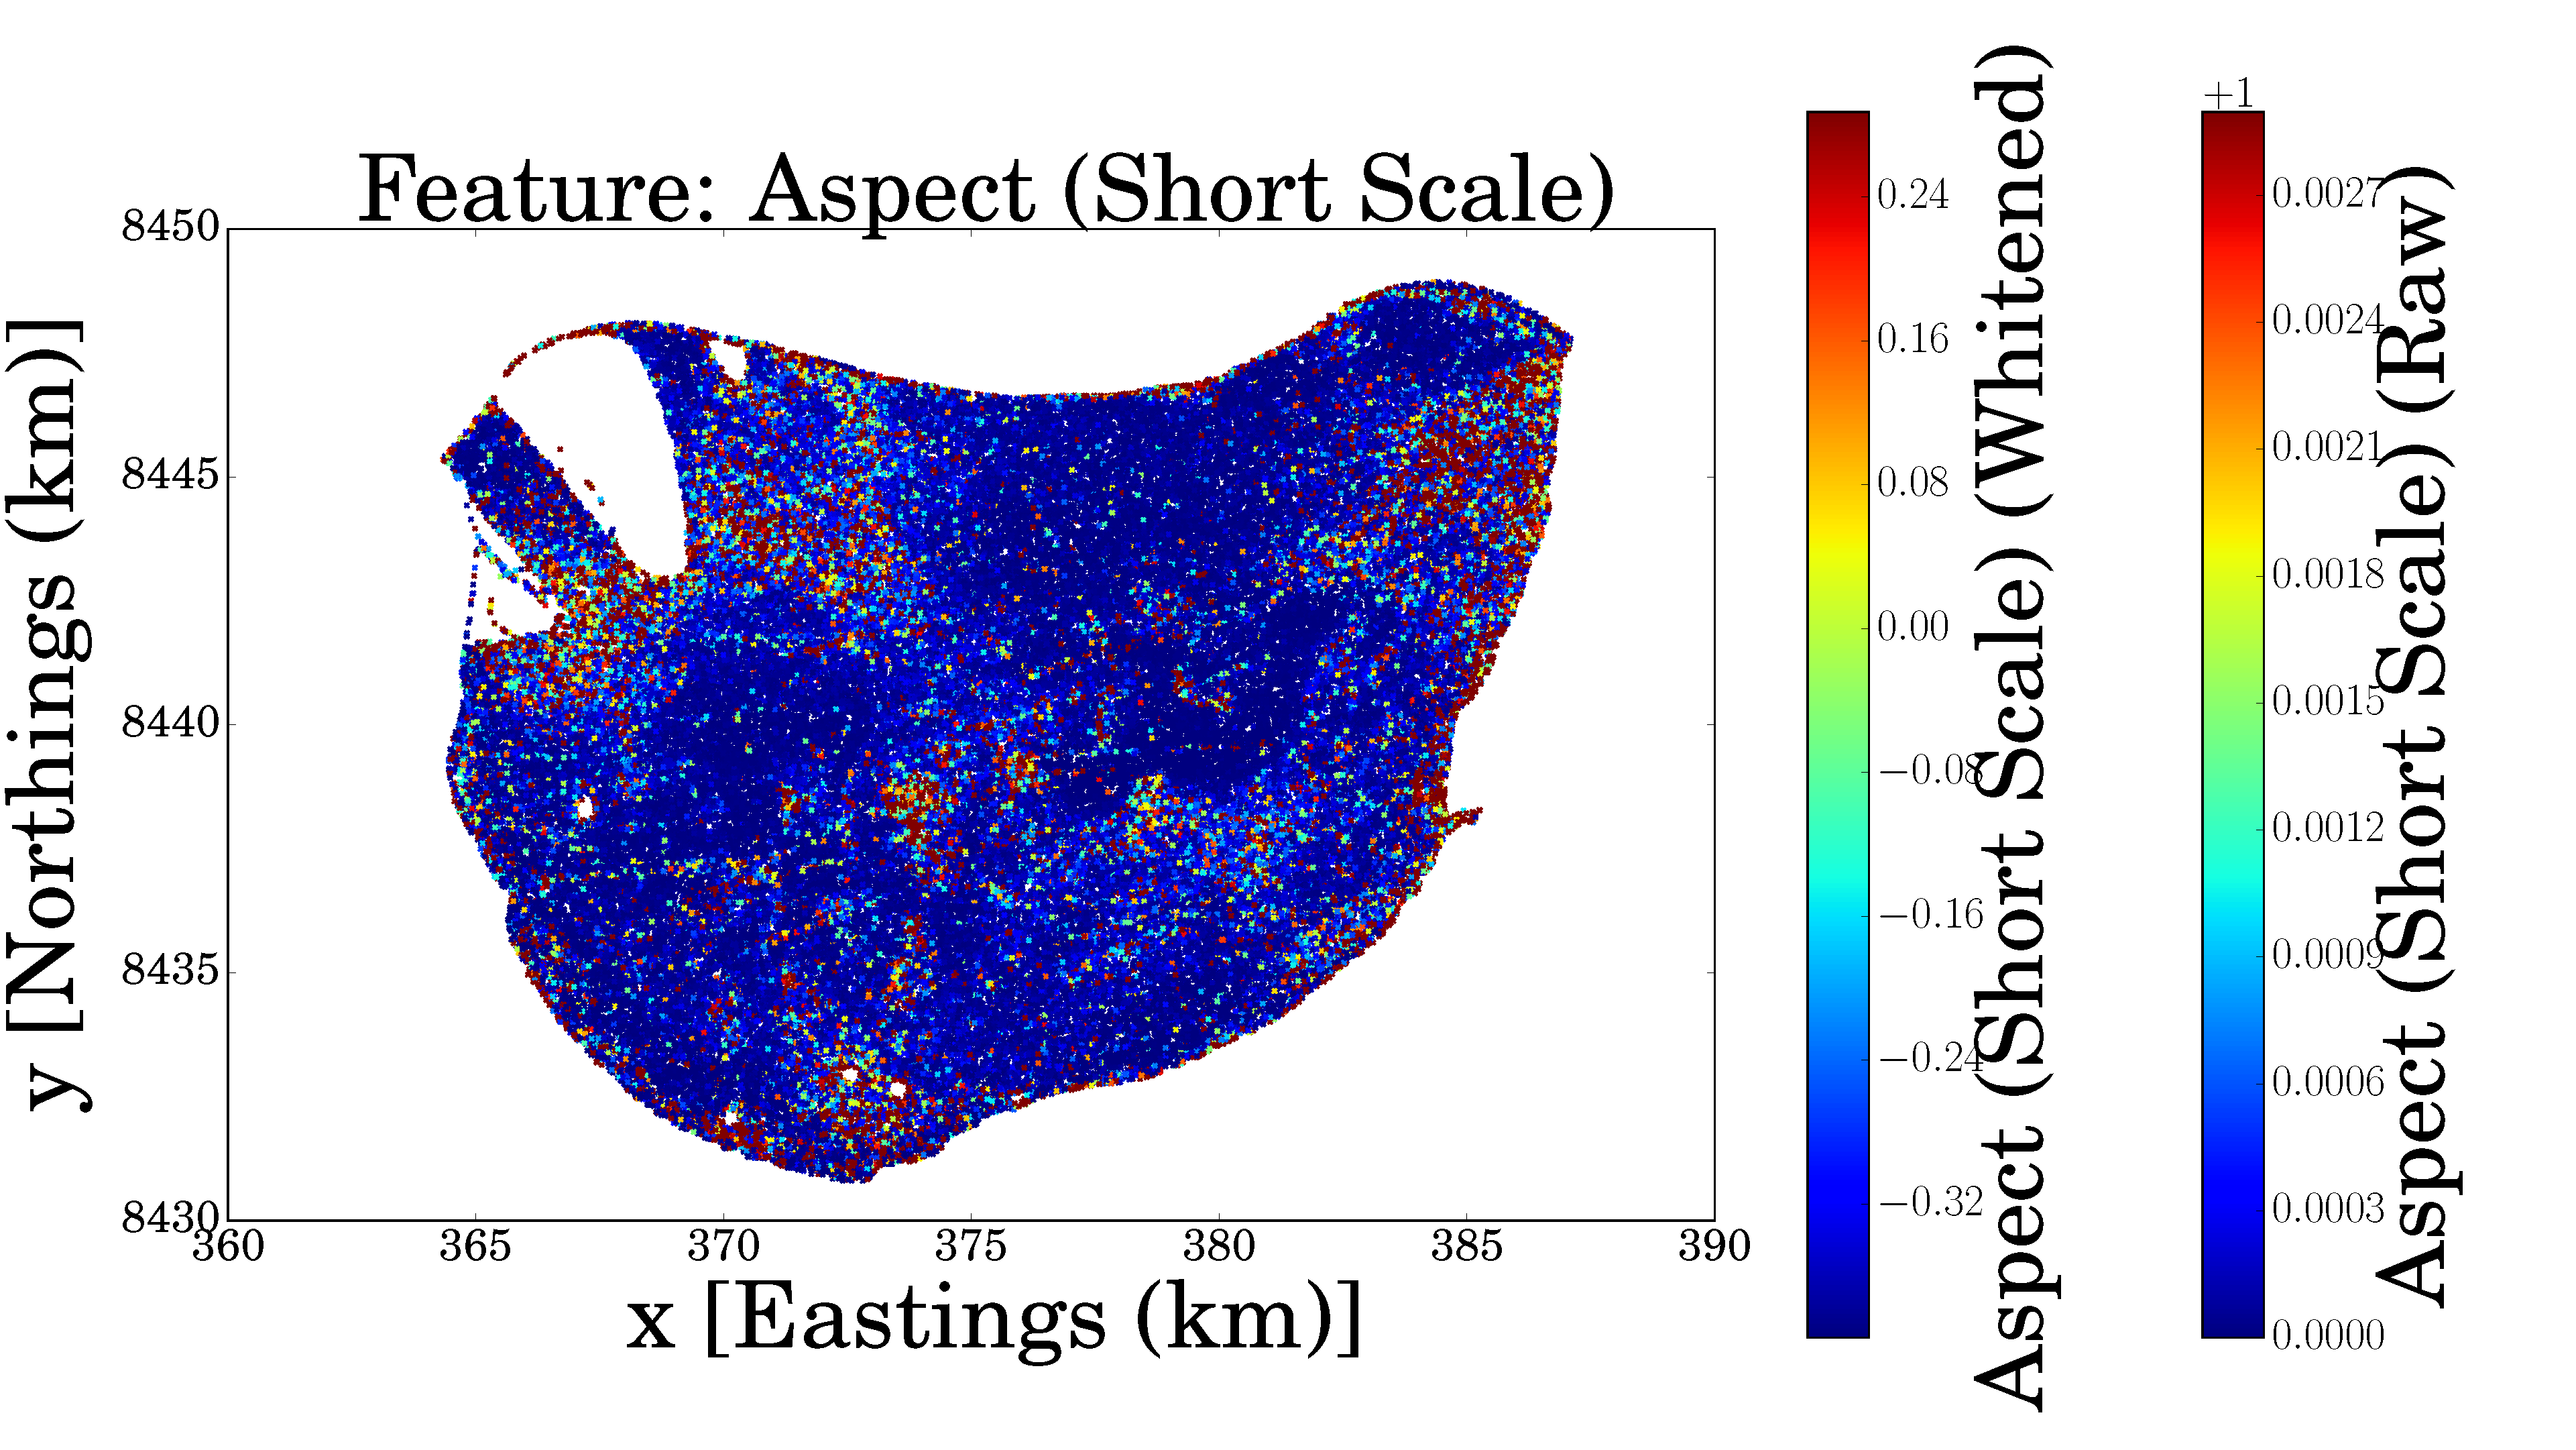
\includegraphics[width = 0.32\linewidth]{Figures/scott_reef_modeling/Figure3-eps-converted-to.png}
		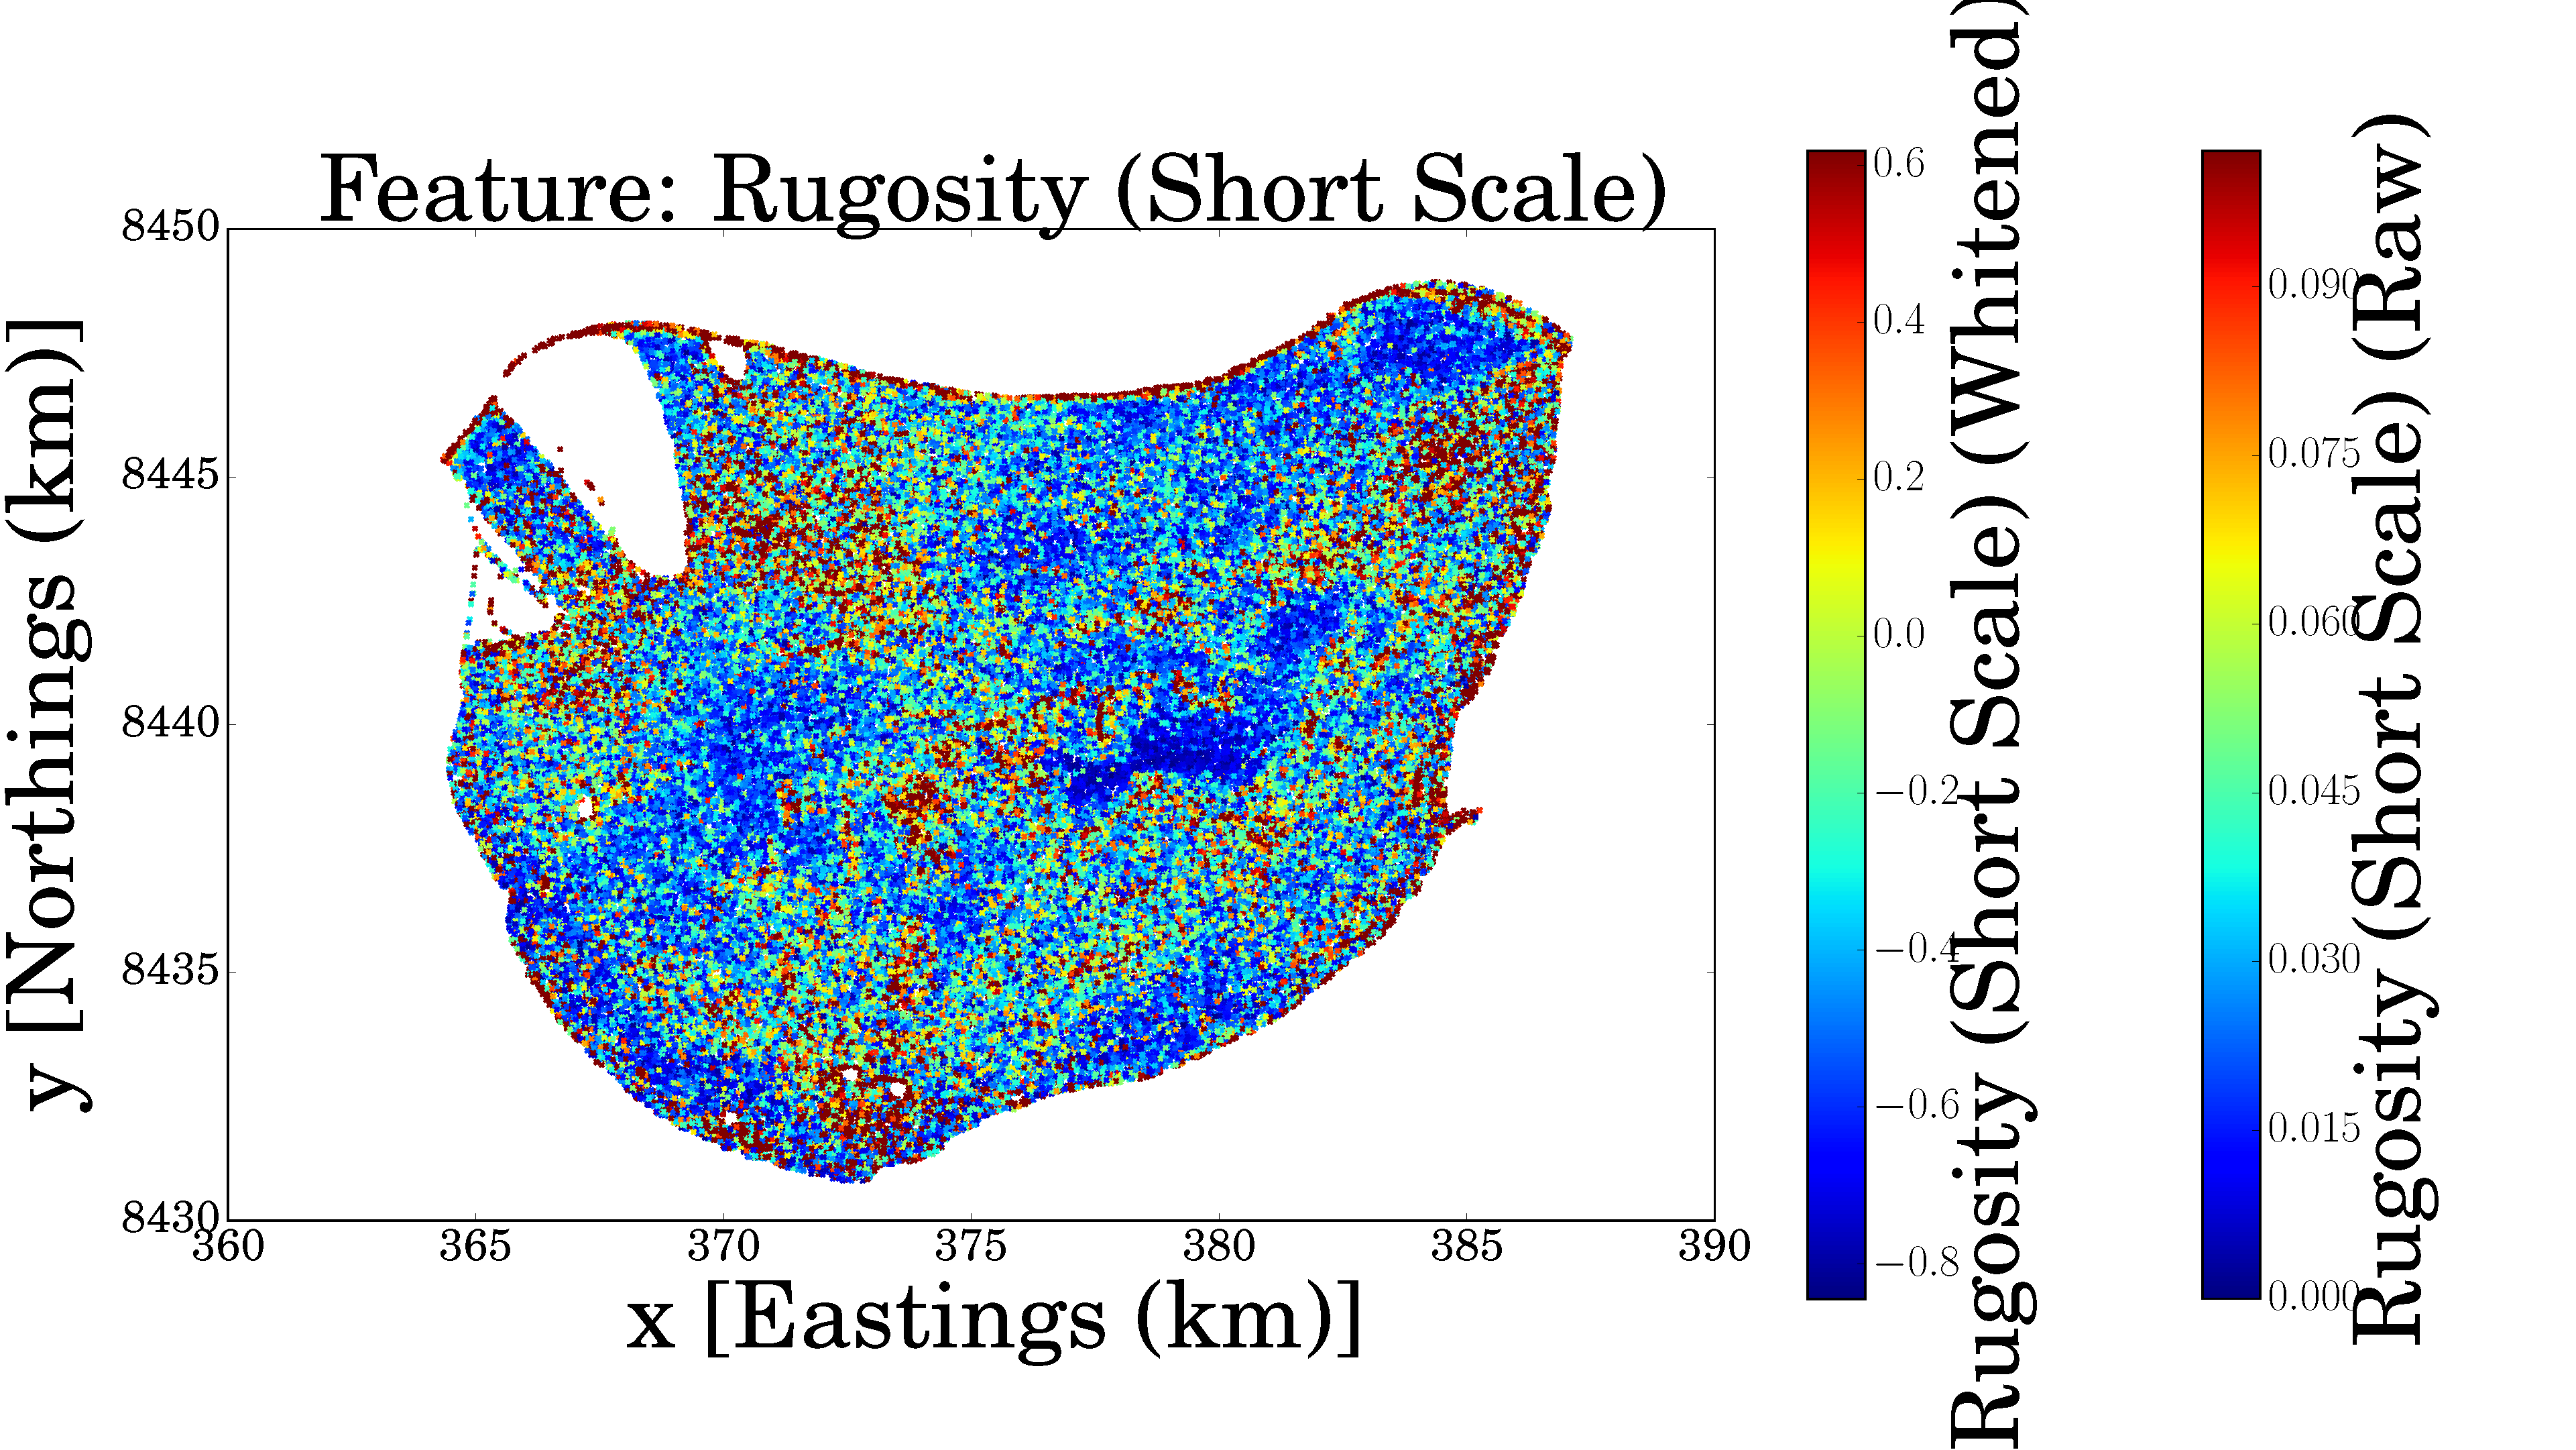
\includegraphics[width = 0.32\linewidth]{Figures/scott_reef_modeling/Figure4-eps-converted-to.png}
		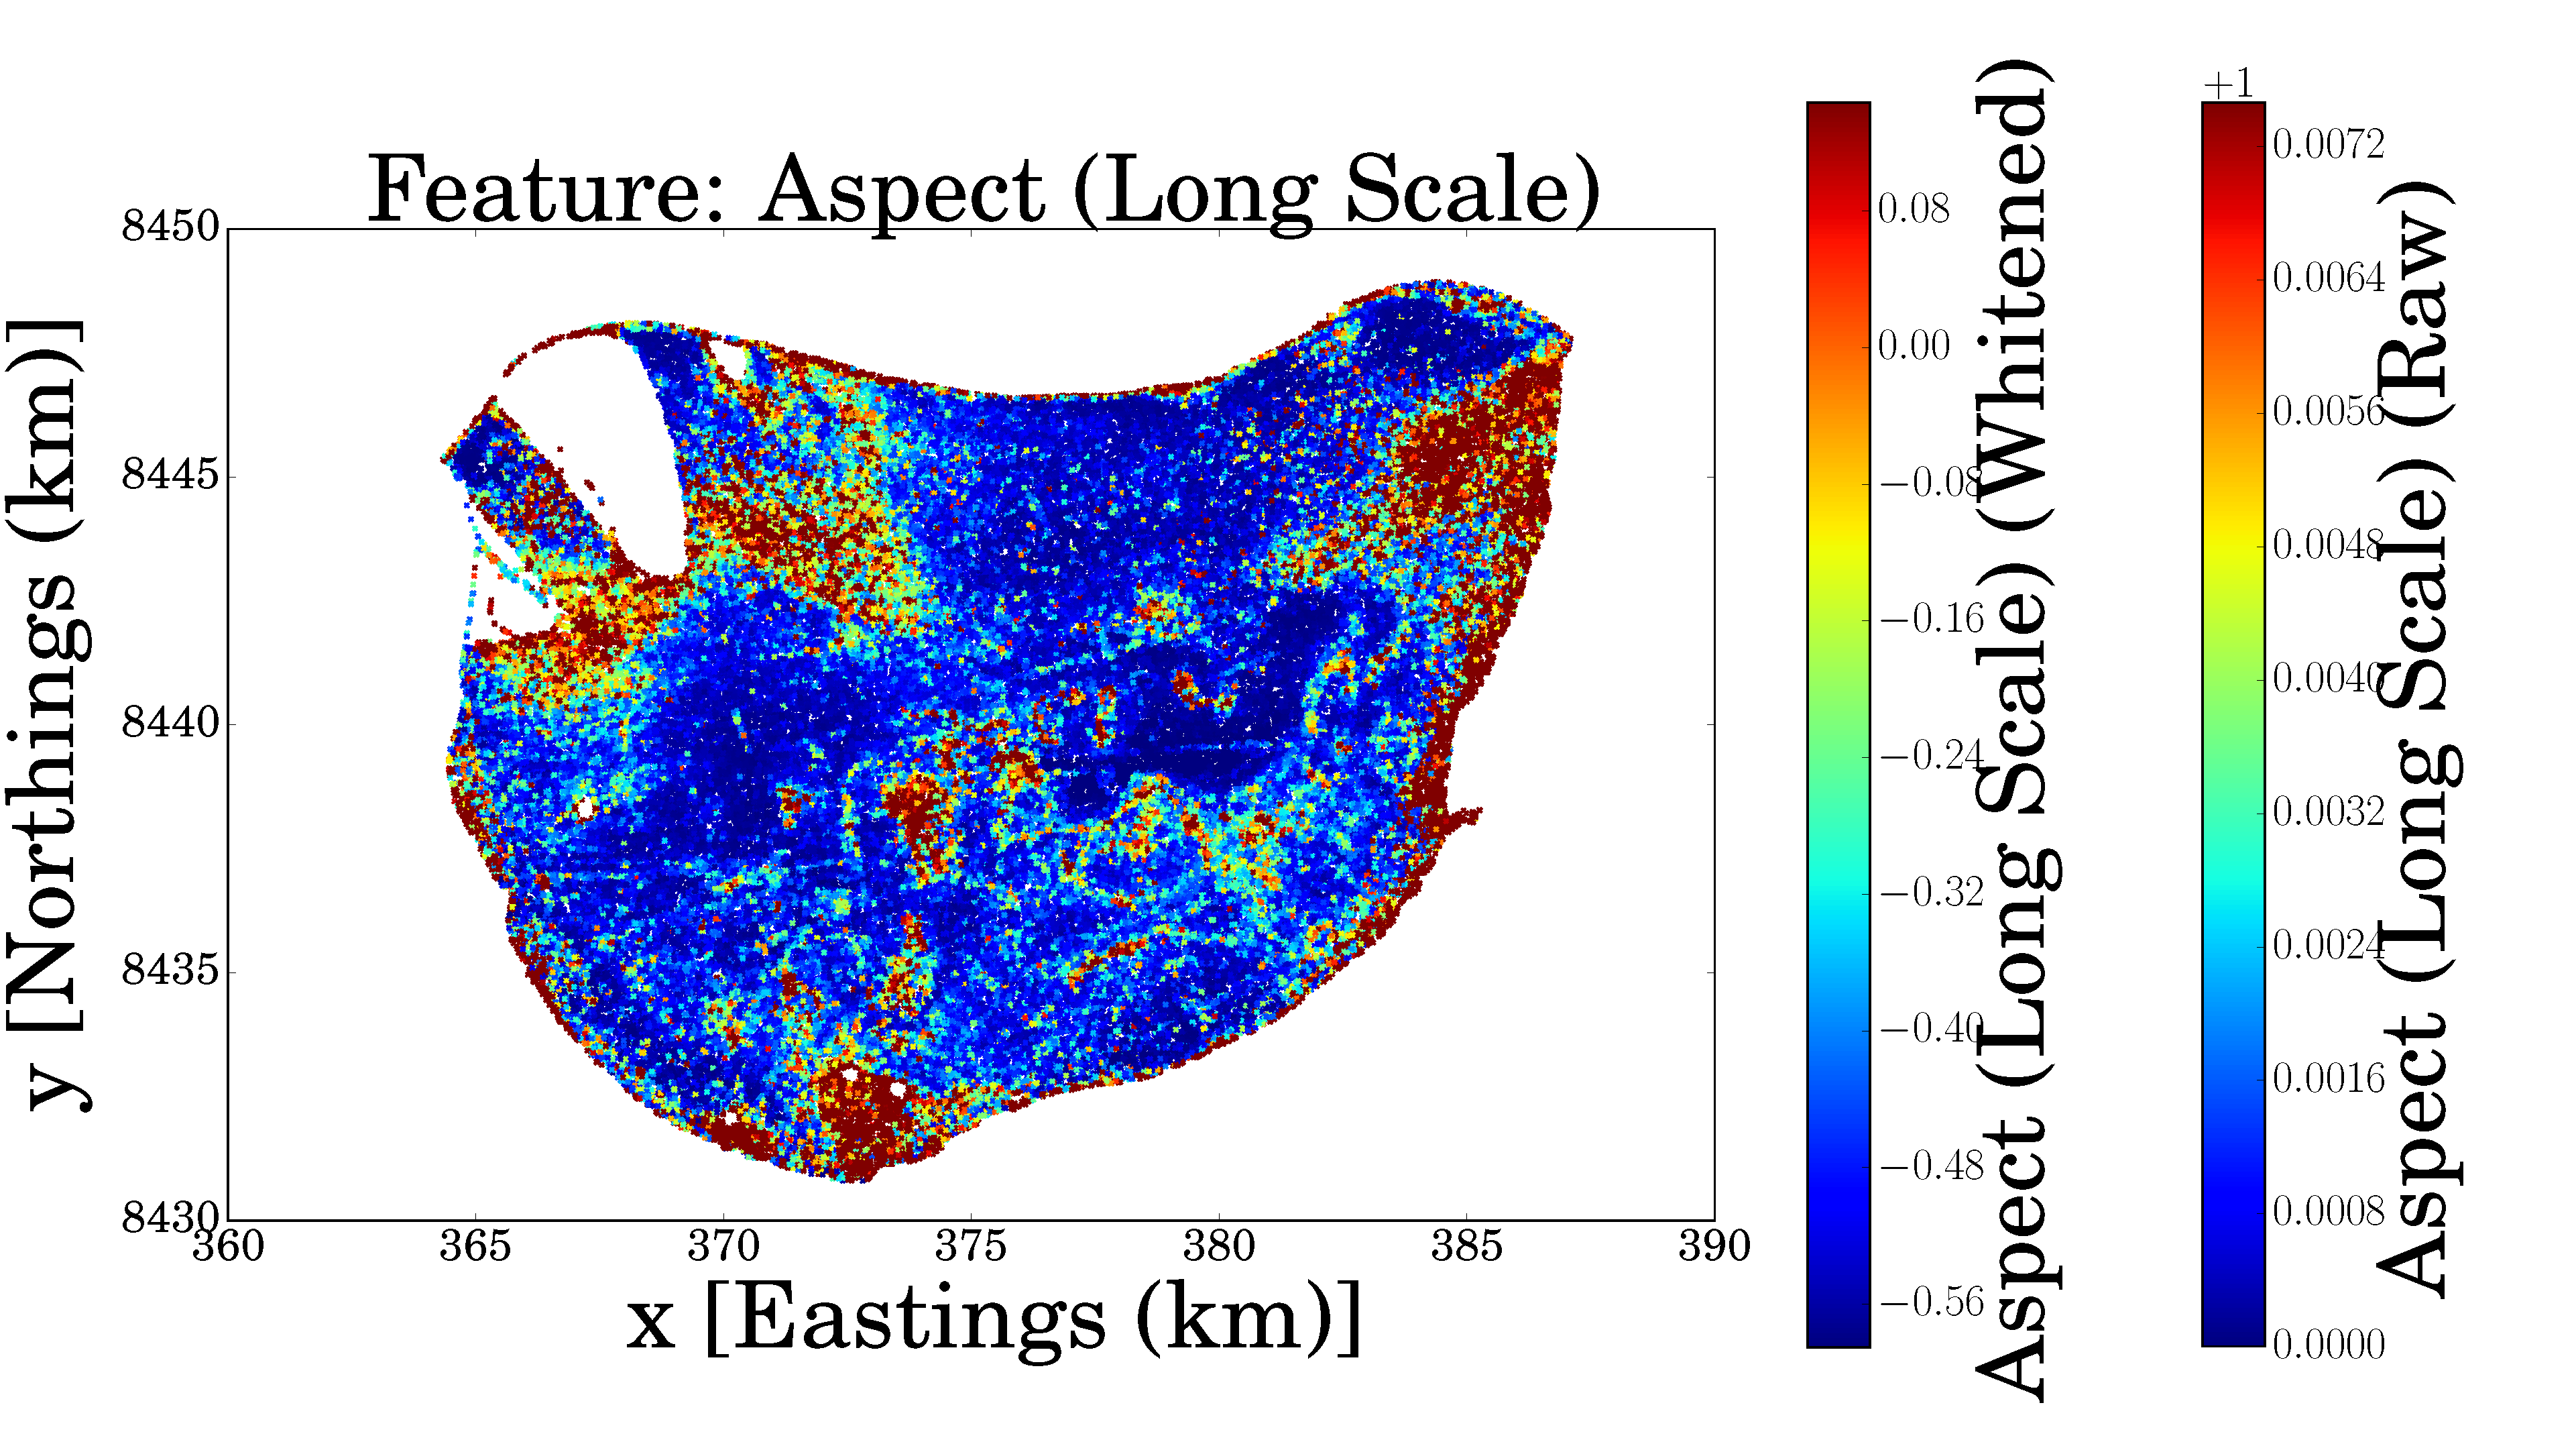
\includegraphics[width = 0.32\linewidth]{Figures/scott_reef_modeling/Figure5-eps-converted-to.png}
		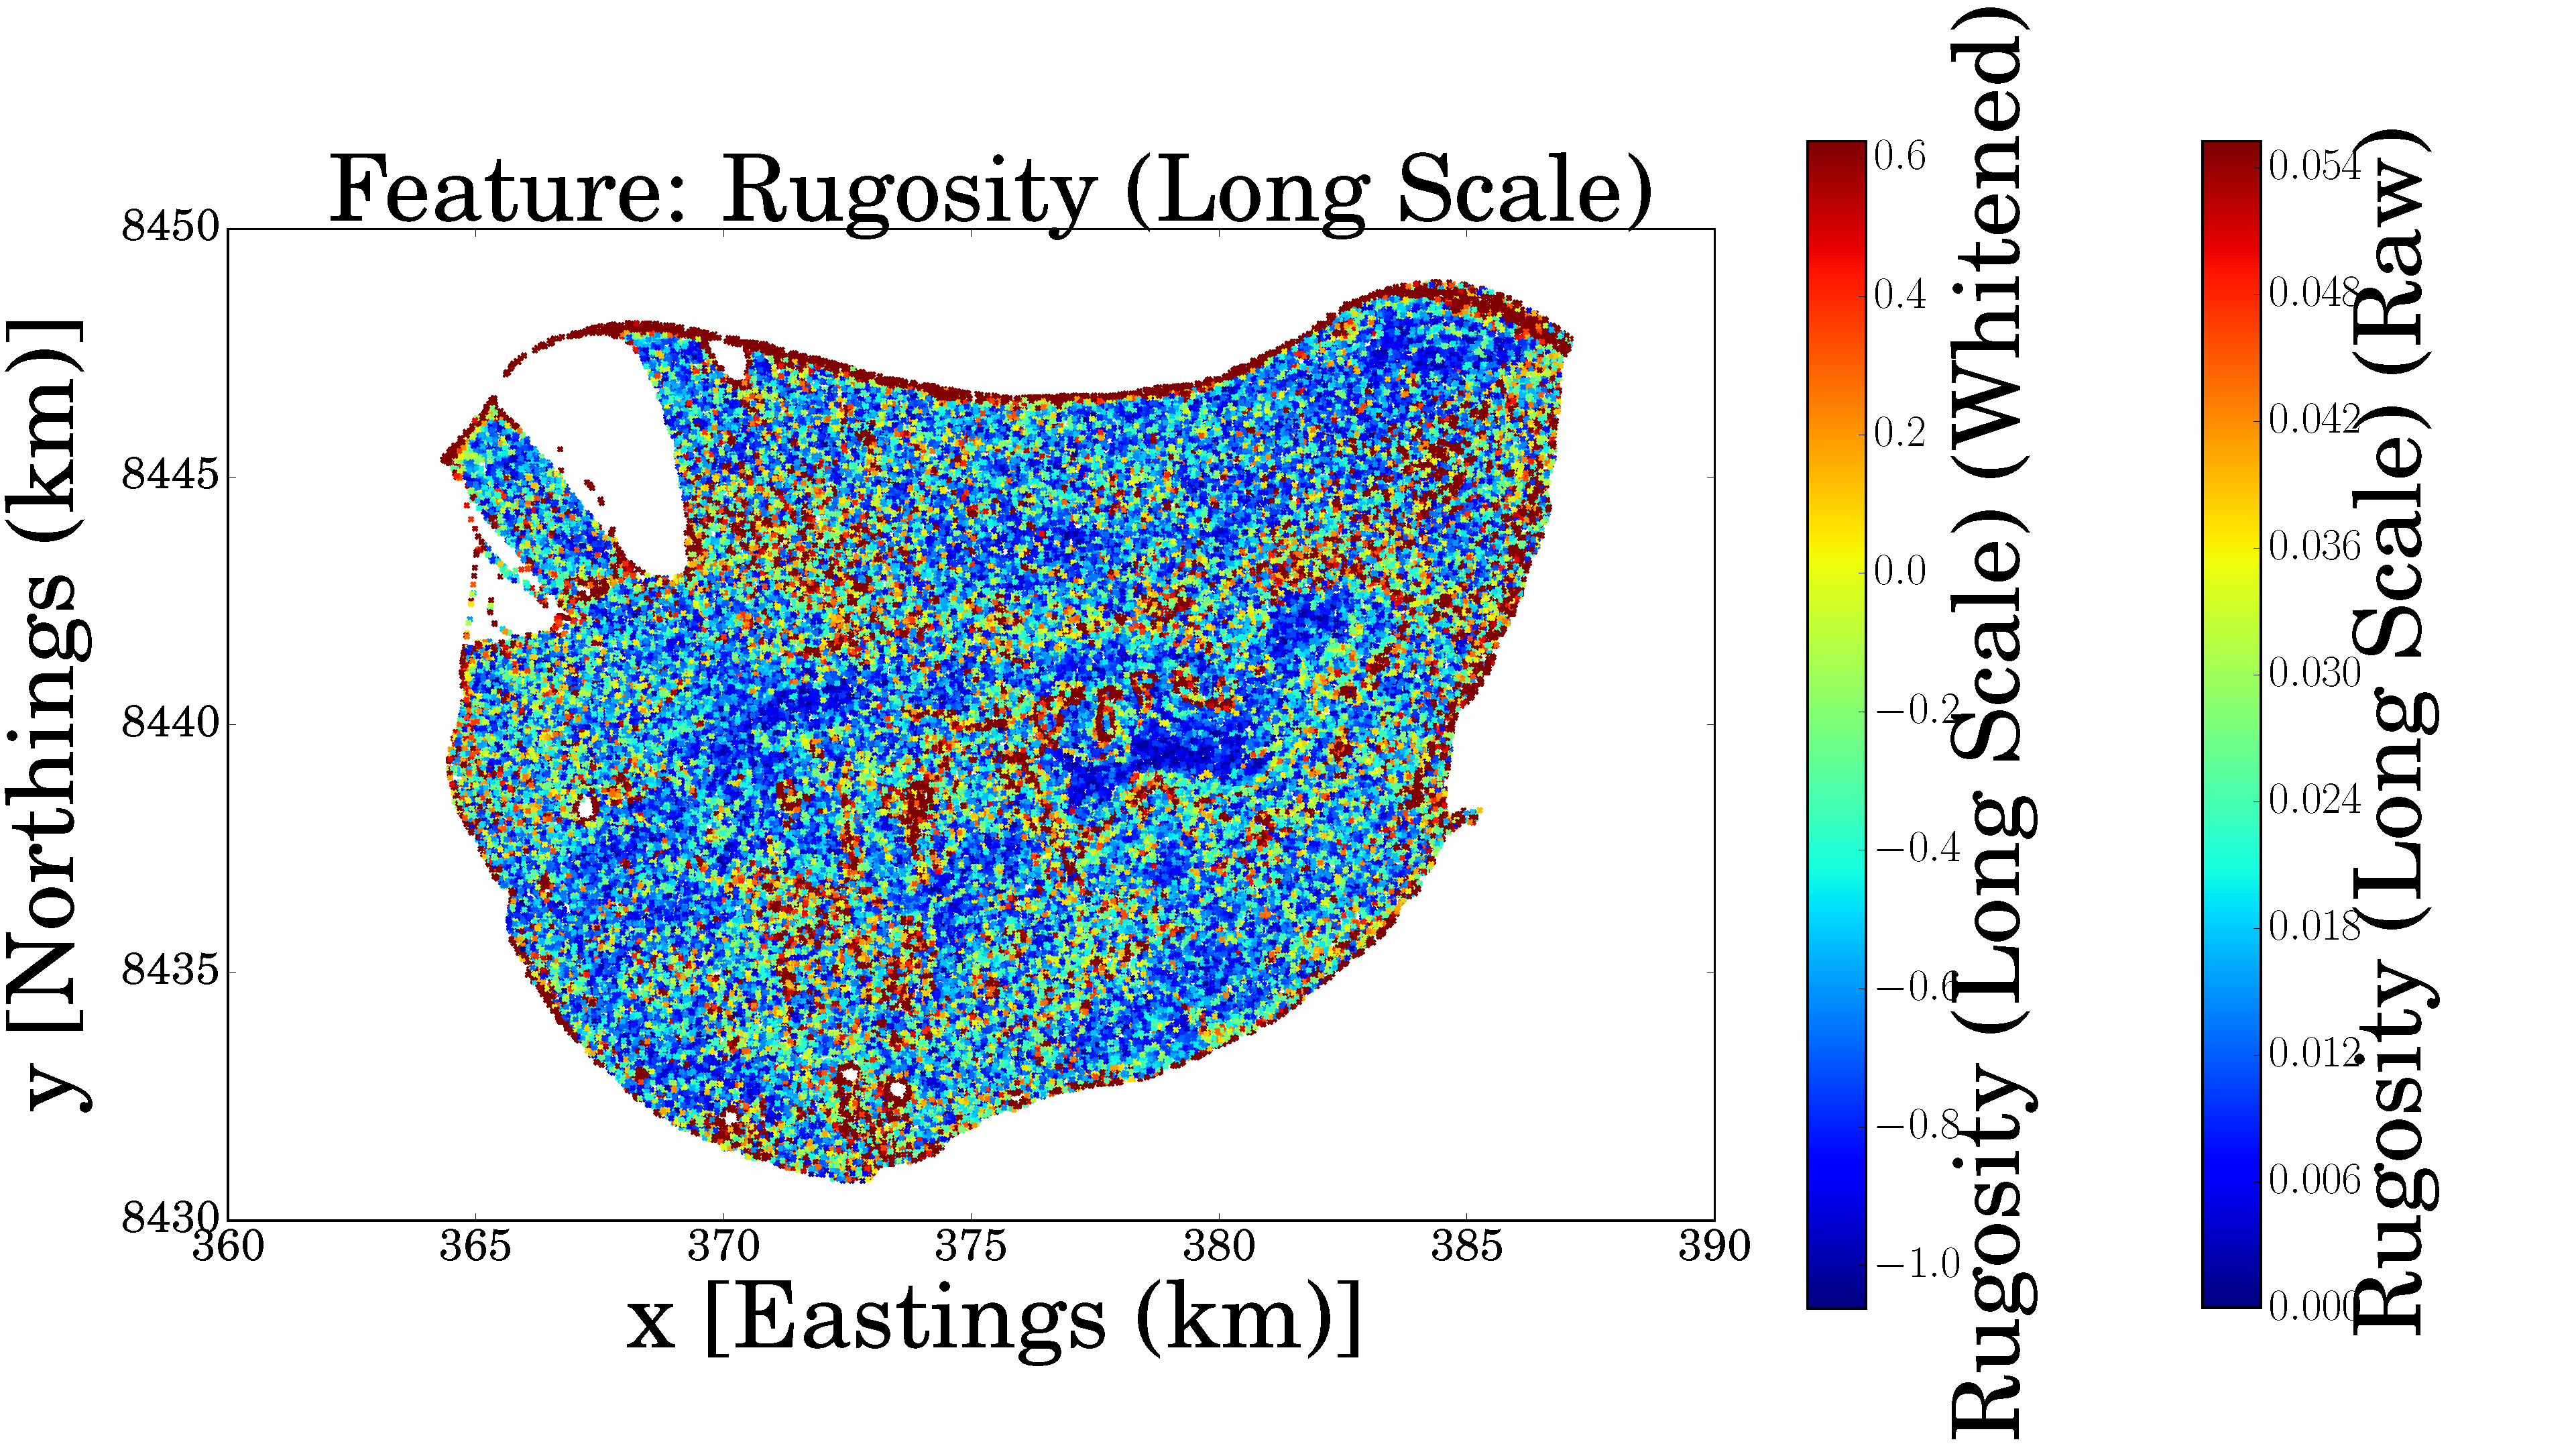
\includegraphics[width = 0.32\linewidth]{Figures/scott_reef_modeling/Figure6-eps-converted-to.png}
	\caption{Scott Reef Bathymetric Features}
	\label{Figure:Results:ScottReefBathymetricFeatures}
	\end{figure*}
	
	\subsection{Formulation and Structure}

		The receding horizon approach requires the selection of a horizon length and the number of control points (query points) for which the path is to be defined upon. The horizon length plays a significant role in the performance of the method. A short horizon length tends to produce paths that are similar to a myopic approach. A horizon length that is too long, however, can be both inefficient and destabilising. For an informative path-planning scenario, looking ahead too far can have diminishing returns in its informativeness, as the vehicle's belief space would be significantly altered by the time it was supposed to follow the original proposed path.

%		\begin{figure}[!htbp]
%		\centering
%			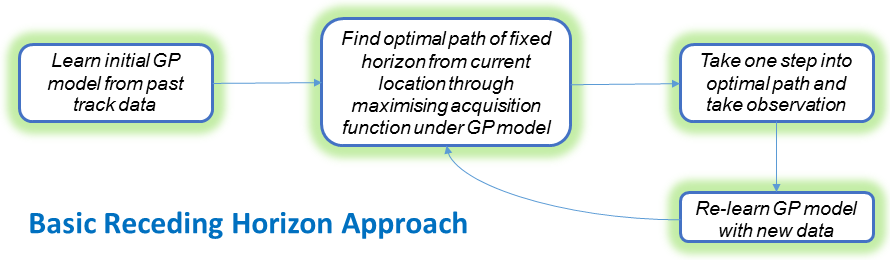
\includegraphics[width = \linewidth]{Figures/receding_horizon_informative_path_planning.png}
%		\caption{Basic Receding Horizon Structure}
%		\label{Figure:Results:RecedingHorizonMethodOutline}
%		\end{figure}
	
		\begin{figure}[!htbp]
			\begin{center}
				\smartdiagramset{text width = 3cm}
				% \smartdiagramset{set color list = {orange!50, green!80, blue!50}}
				\smartdiagram[circular diagram:clockwise]{Learn GP model from collected data, Compute finite optimal path, Move to first control point \& record observation}
			\end{center}
		\caption{Basic Receding Horizon Structure}
		\label{Figure:Results:RecedingHorizonMethodOutline}
		\end{figure}
				
		Figure \ref{Figure:Results:RecedingHorizonMethodOutline} describes the basic flow of the receding horizon approach approach, which resembles the technique of model predictive control (MPC) in control theory. That is, it computes an optimal policy of finite horizon in each time step, and only executes the first action from the policy. The acquisition function to be maximised in each step is flexible, and we compare LDE acquisition \eqref{Section:LinearisedEntropy:Equation:MulticlassLinearisedEntropy} against MCJIE acquisition and other acquisition functions under the receding horizon structure in the next section. In each time step, a new path of a certain horizon length is proposed, which is discretised into a finite set of control points. The vehicle only executes the policy towards the first control point while recording observations. It then relearns the GP classifier model with new observations, and repeats the process. 
		
\section{Experimental Results}
\label{Section:ExperimentalResults}

	In this section we demonstrate the performance of LDE acquisition under a receding horizon structure. We compare the results to path planning under other acquisition functions, as well as myopic approaches. Under a misclassification performance criterion, we show that LDE acquisition achieves stable and desirable results, and experimentally outperform competing methods.
	
	We test our approach on the Scott Reef data set provided by \incite{IMOS}. The benthic labels are obtained through unsupervised clustering on benthic imagery using Gaussian latent Dirichlet allocation (LDA) \cite{Steinberg2015128}, producing 22 unique benthic class labels, with 17 of them associated with identifiable semantic meaning and the rest either over-exposed or under-exposed in lighting. 

	\subsection{Modeling Scott Reef Benthic Zones}
		
		An OVA GP multiclass classifier is to model the benthic habitats using five bathymetric features - bathymetric depth, aspect (short scale), rugosity (short scale), aspect (long scale), and rugosity (long scale) (figure \ref{Figure:Results:ScottReefBathymetricFeatures}). It is assumed that the nature of the habitat depends on the location implicitly through explicit dependence on bathymetric structure of the seafloor. Thus, spatial coordinates are not included in the feature set. As training labels are only available around past mission tracks (figure \ref{Figure:Results:ScottReefBathymetricFeatures}), a synthetic ground truth is generated separately in order to assess the relative performance between path-planning techniques (figure \ref{Figure:Results:ScottReefSyntheticGroundTruth}). Note that this ground truth is generated in accordance to the limited training labels available in the dataset and does not necessary represent the physical reality at Scott Reef. 

		\begin{figure}[t]
		\fontsize{24}{12}\selectfont
		\centering
			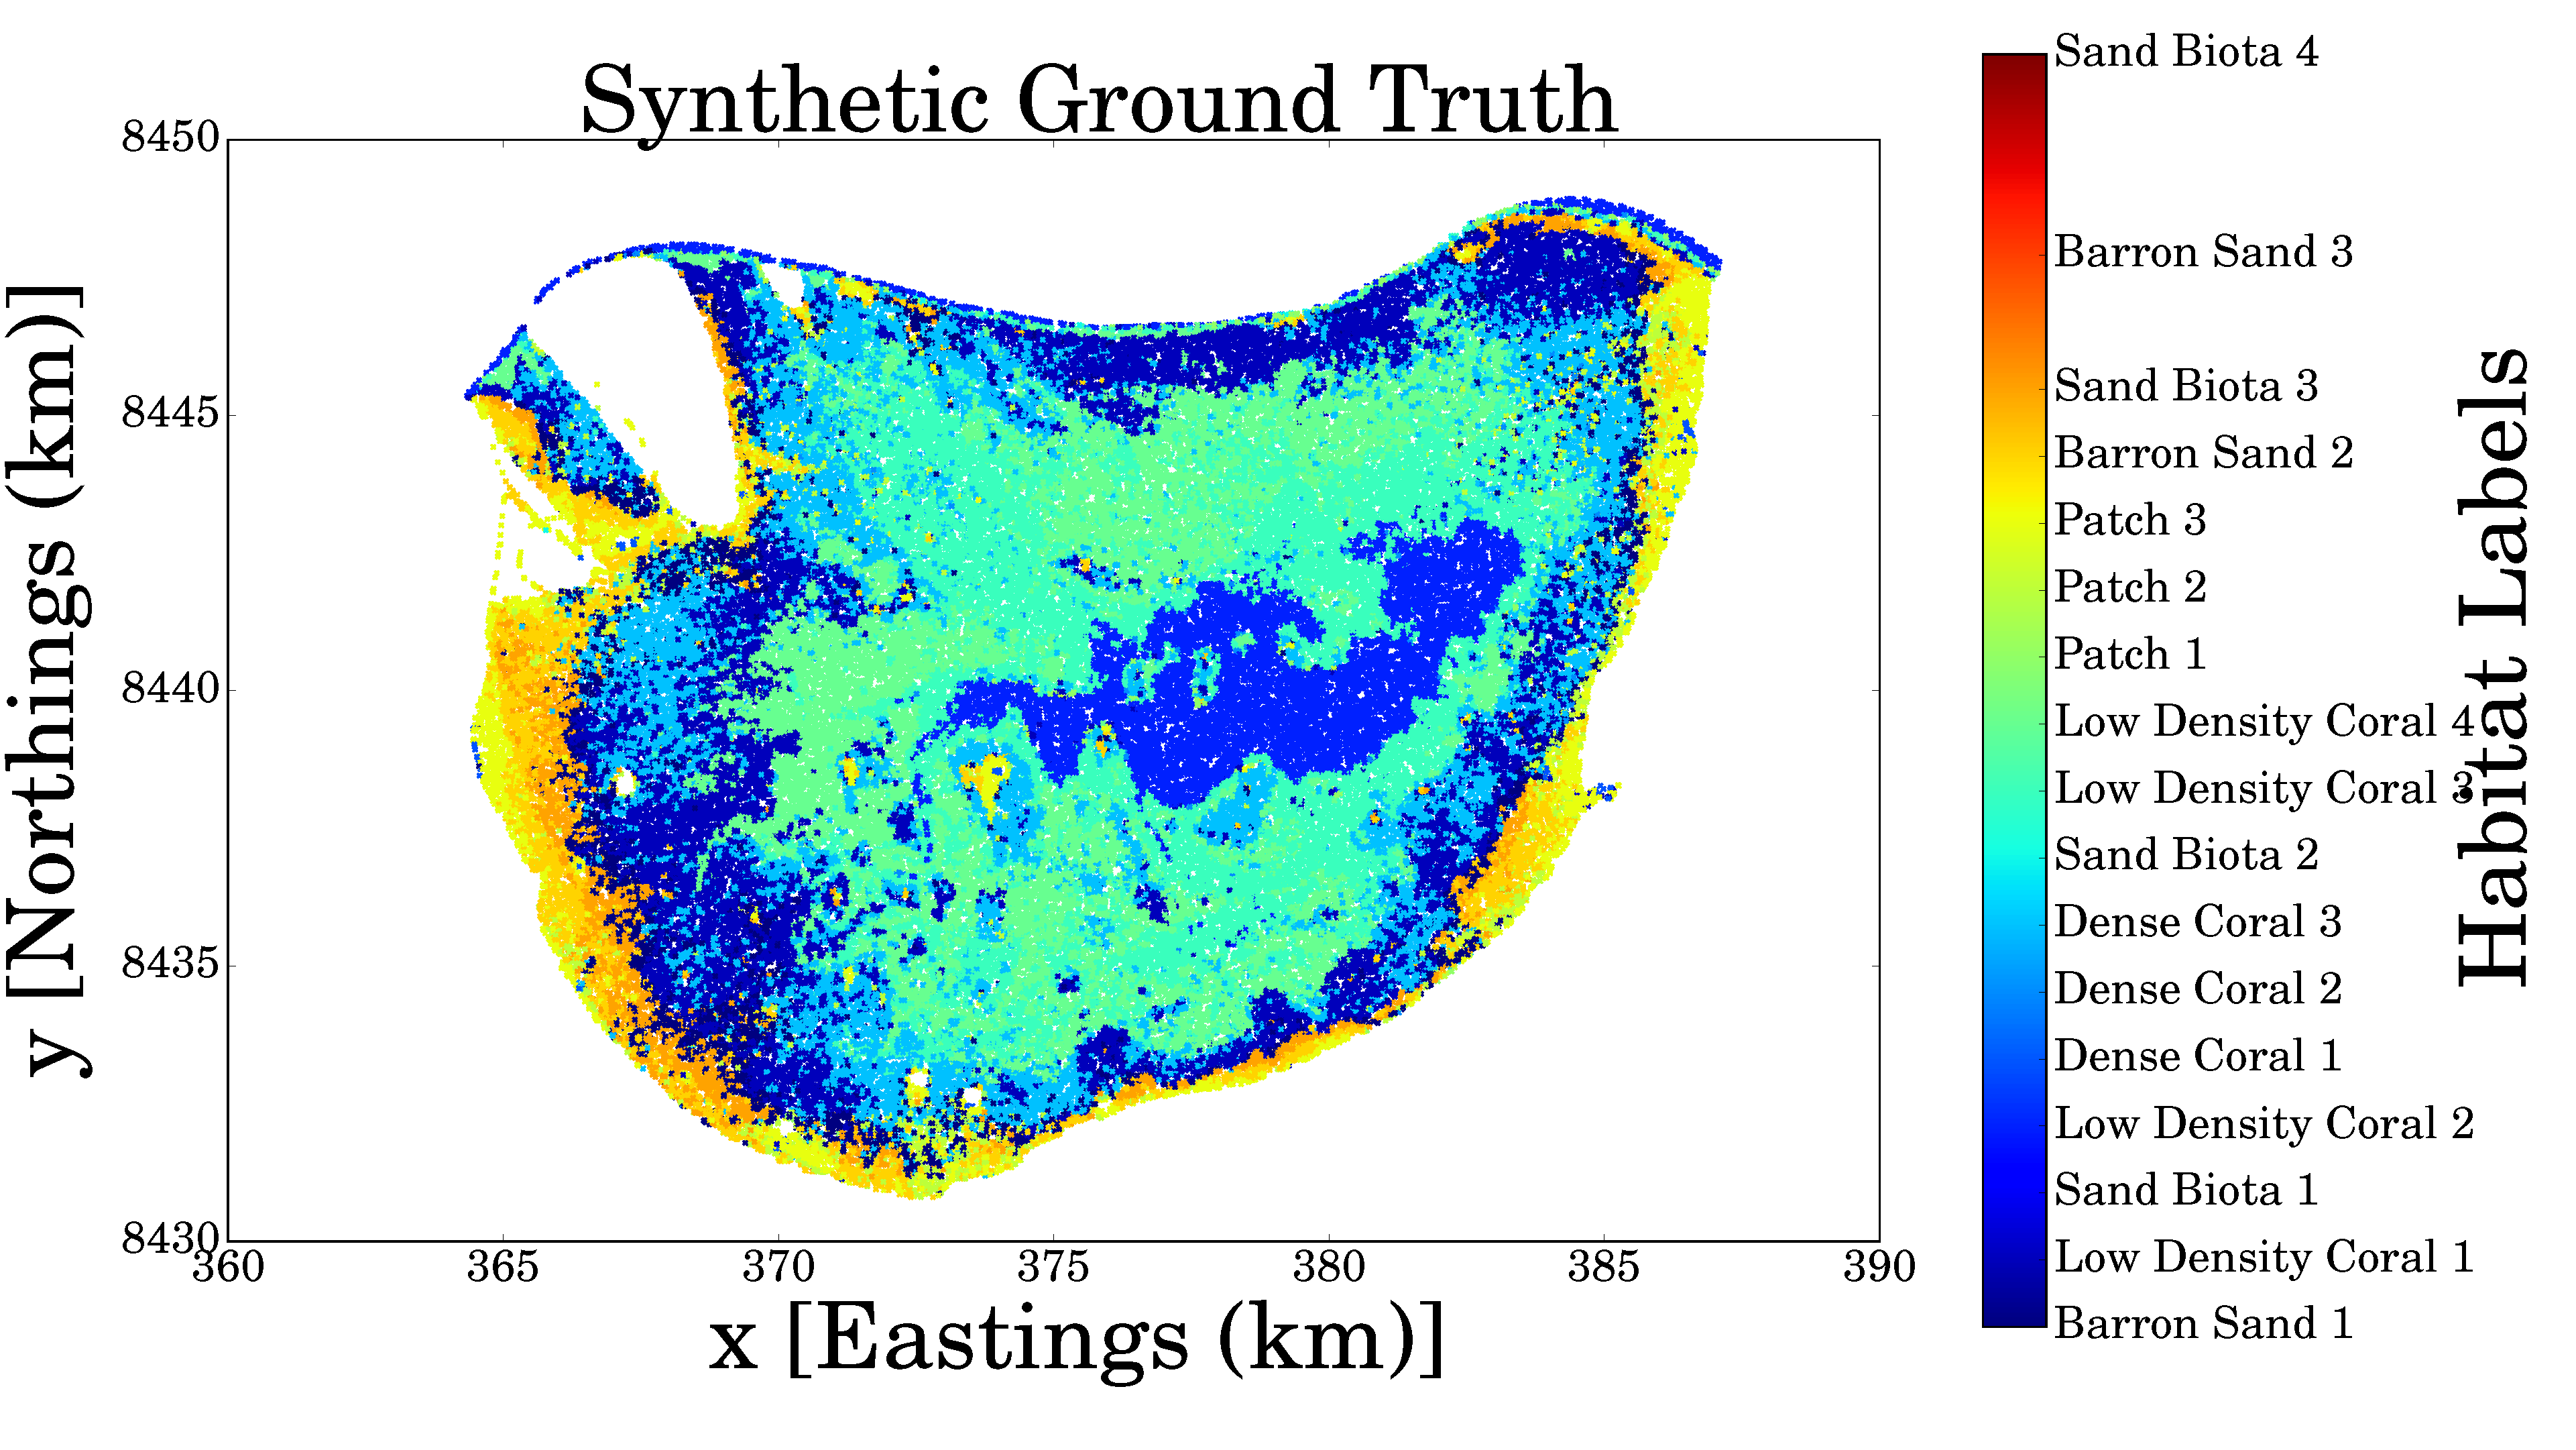
\includegraphics[width = \linewidth]{Figures/scott_reef_modeling/Figure7-eps-converted-to.png}
		\caption{Scott Reef: Synthetic Ground Truth}
		\label{Figure:Results:ScottReefSyntheticGroundTruth}
		\end{figure}
		
		\begin{figure}[bp]
		\centering
			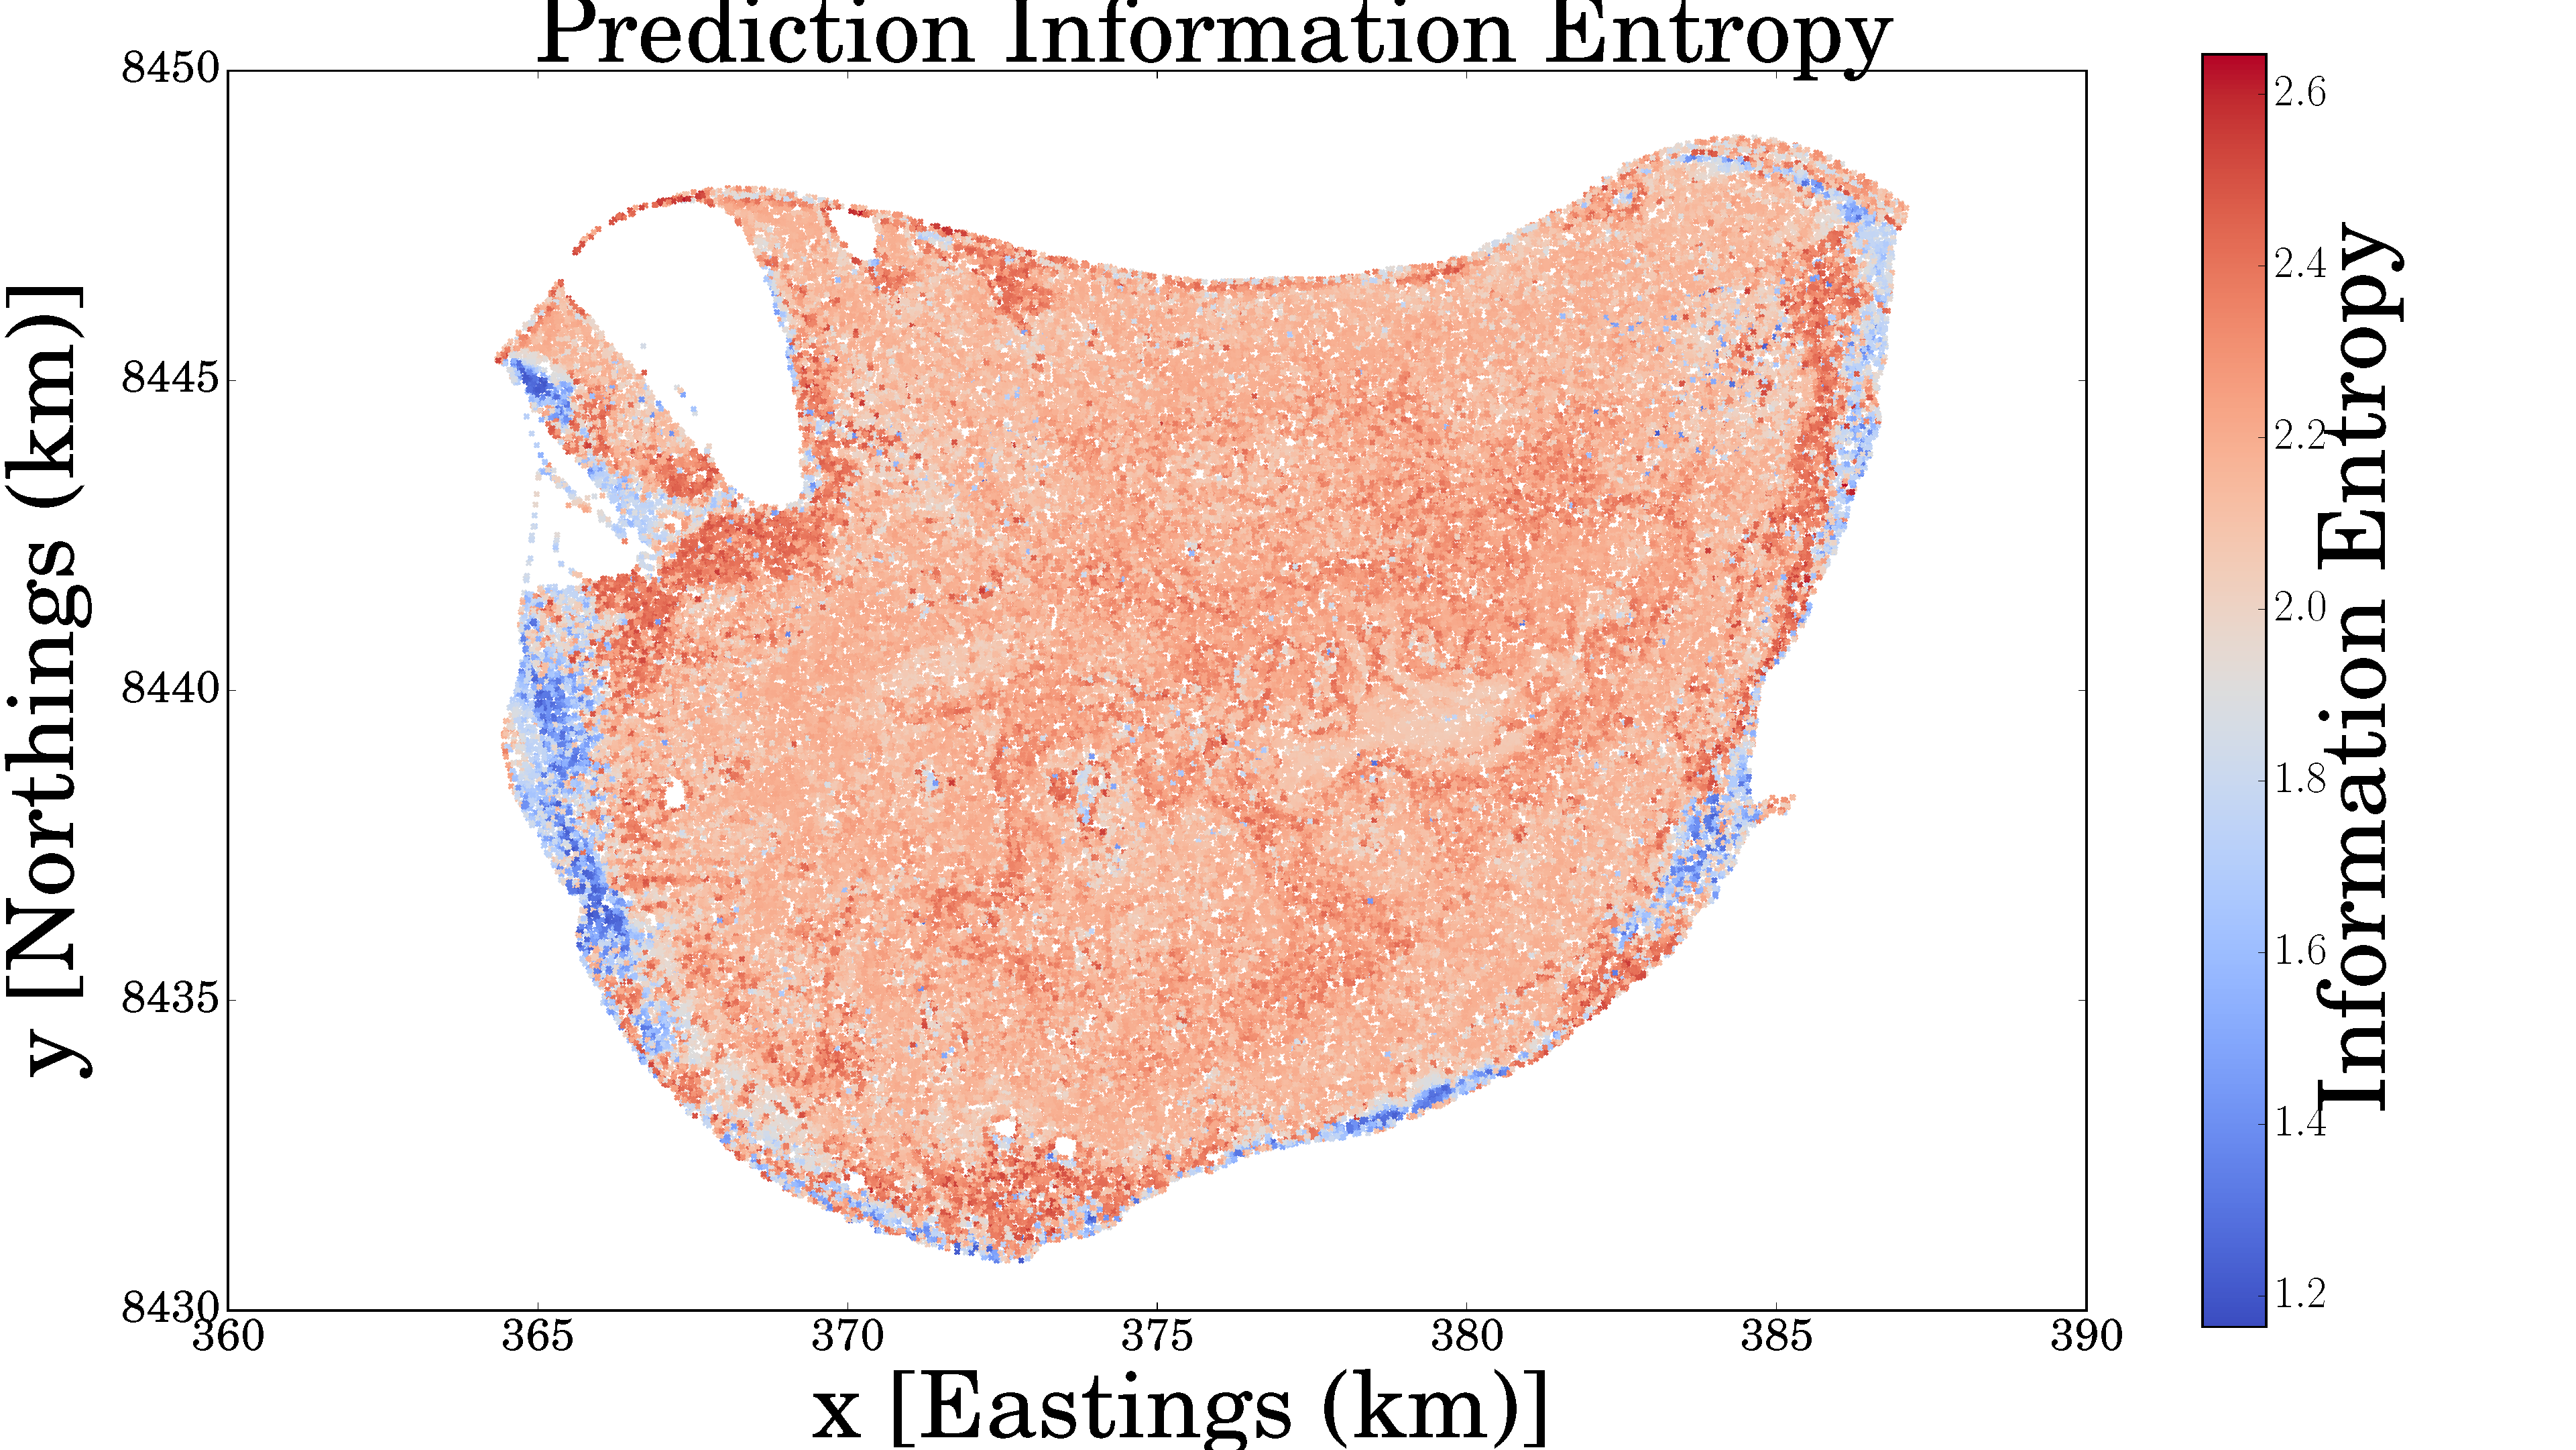
\includegraphics[width = \linewidth]{Figures/scott_reef_modeling/Figure9-eps-converted-to.png}
		\caption{Scott Reef: Prediction Information Entropy}
		\label{Figure:Results:ScottReefPredictionInformationEntropy}
		\end{figure}
				
		To reduce computational requirements, 200 training points were sampled from those tracks for initial modeling, which achieves a 41.54\% misclassification rate, or 58.46\% prediction accuracy (figure \ref{Figure:Results:ScottReefInitialPredictions}). This demonstrates the advantage of modeling the benthic environment upon a bathymetric feature space instead of spatial coordinates. The tracks cover less than 5\% of the region, yet more than half of the region can be accurately modeled with such scarce data. This model takes advantage of the fact that although habitats can be far away spatially, they can have similar bathymetric structures such that they are close in the bathymetric feature space.

		While we can map the reef with an accuracy of 58.46\% using only 200 training points (figure \ref{Figure:Results:ScottReefInitialPredictions}), the prediction information entropy is rather uniformly high (figure \ref{Figure:Results:ScottReefPredictionInformationEntropy}) due to the scarcity of data. In this initial scenario, under the prediction information entropy criterion the vehicle would simply try to map out all regions as much as possible - a very costly policy.
		
		\begin{figure}[t]
		\centering
			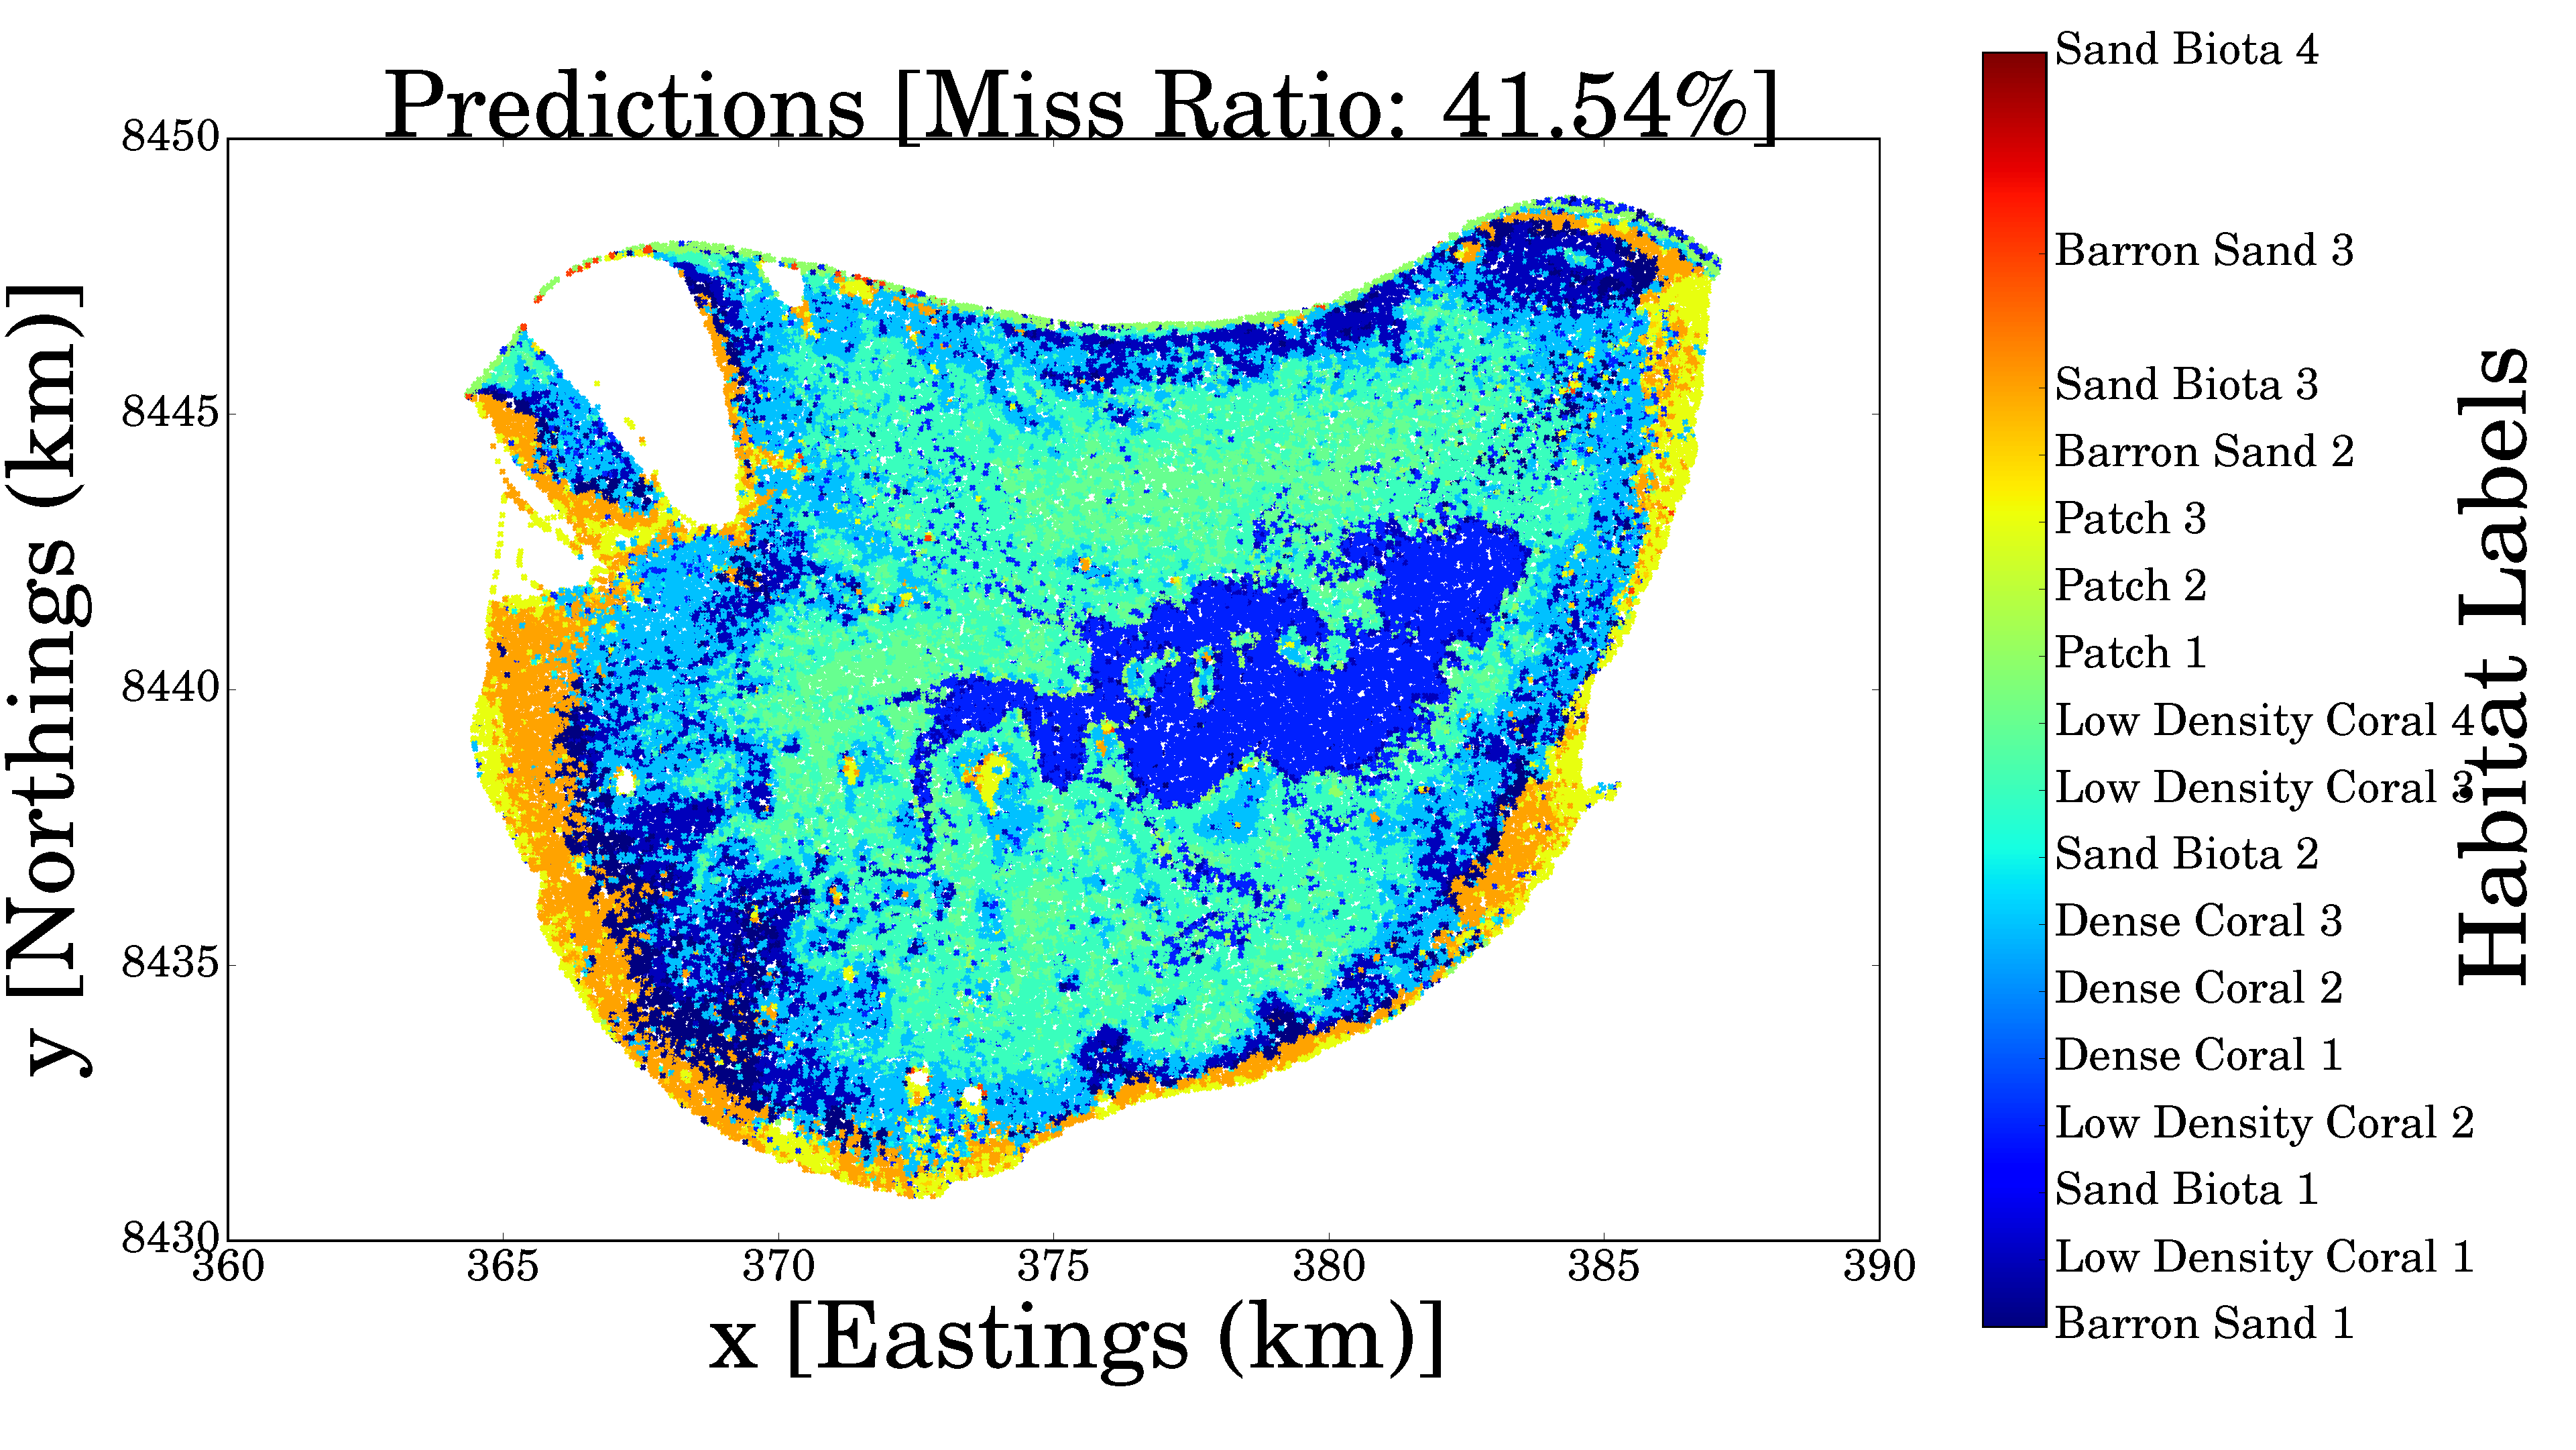
\includegraphics[width = \linewidth]{Figures/scott_reef_modeling/Figure8-eps-converted-to.png}
		\caption{Scott Reef: Initial Prediction}
		\label{Figure:Results:ScottReefInitialPredictions}
		\end{figure}
					
		The linearised differential entropy, however, emphasizes on the places where the vehicle should first focus on (figure \ref{Figure:Results:ScottReefLinearisedDifferentialEntropy}). Comparing this with the bathymetric features (figure \ref{Figure:Results:ScottReefBathymetricFeatures}), we can deduce that the vehicle would focus on places with the highest and lowest depths.
		
		\begin{figure}[bp]
		\centering
			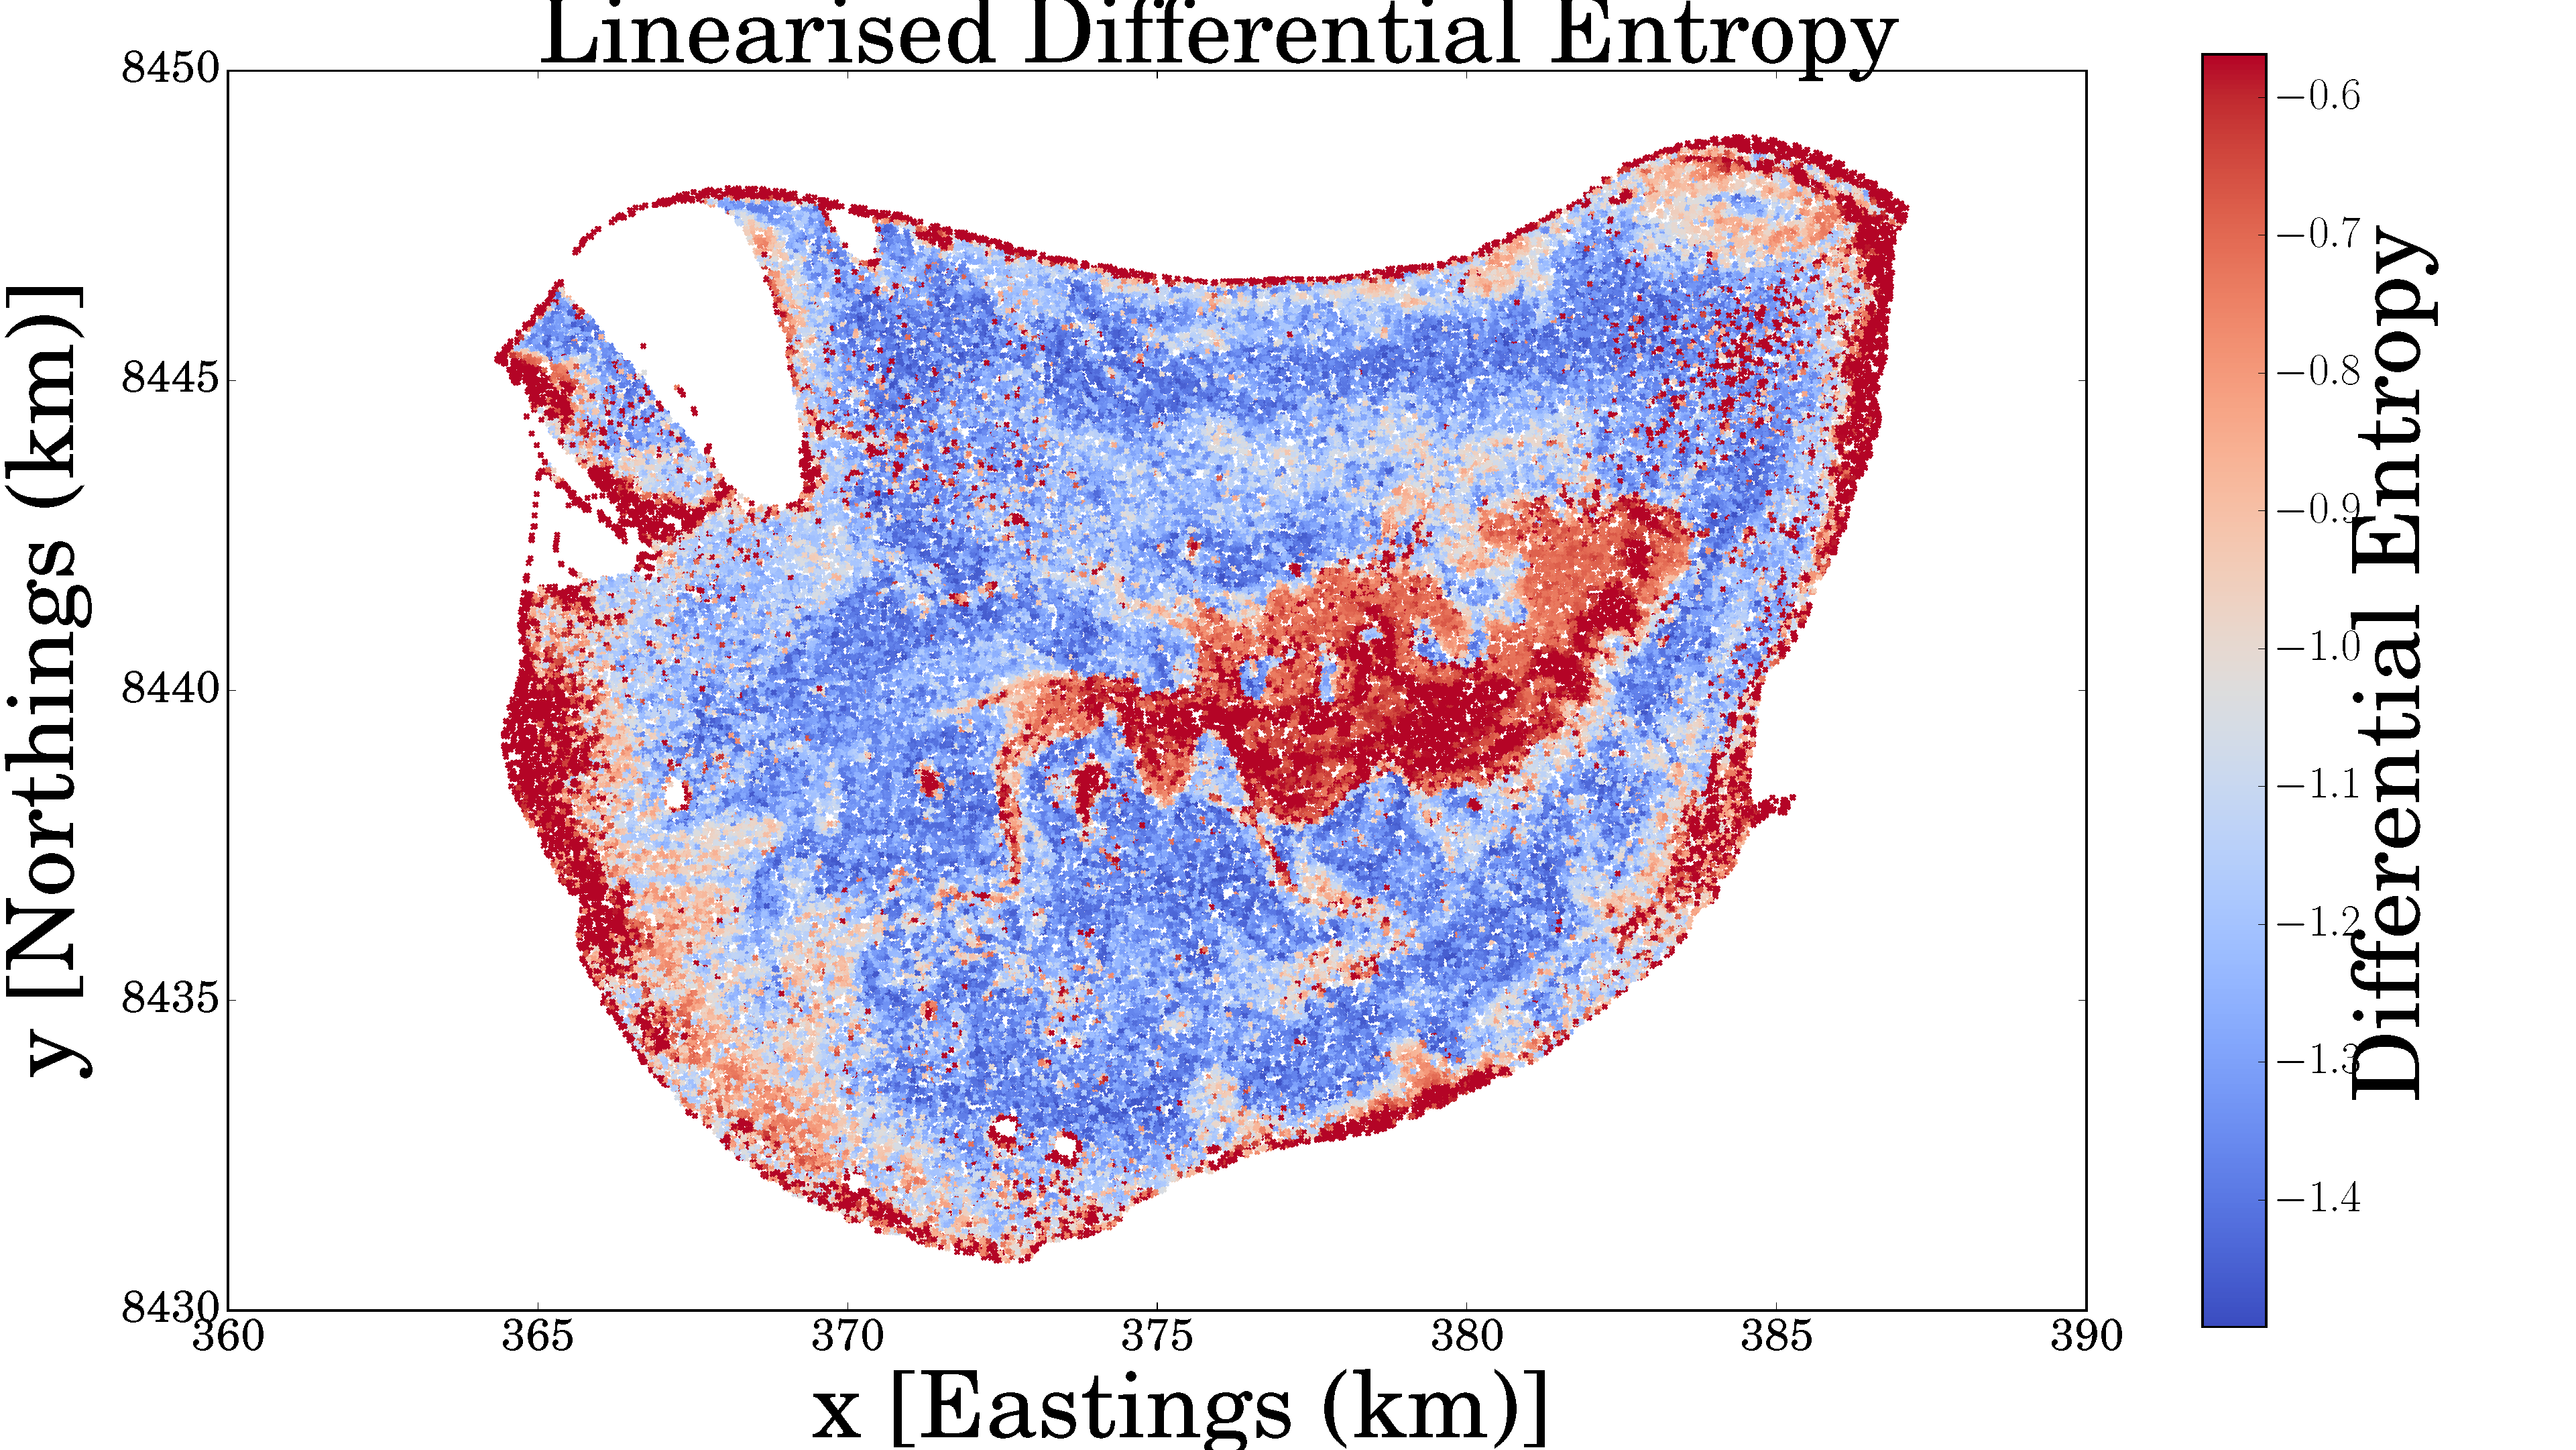
\includegraphics[width = \linewidth]{Figures/scott_reef_modeling/Figure11-eps-converted-to.png}
		\caption{Scott Reef: Linearised Differential Entropy}
		\label{Figure:Results:ScottReefLinearisedDifferentialEntropy}
		\end{figure}
	
%		While these visualisations compare only the marginalised entropies at each query point, the main advantage of using linearised differential entropy as the acquisition function is that the joint linearised differential entropy between an arbitrary set of query points can be readily computed in a straight forward way by \eqref{Section:LinearisedEntropy:Equation:BinaryLinearisedEntropy} and \eqref{Section:LinearisedEntropy:Equation:MulticlassLinearisedEntropy}. On the other hand, there are no closed form for the joint prediction information entropy, so one would have to use Monte Carlo sampling to estimate the joint distributions. Thus, the accuracy of the mutual entropy measure would depend on the number of sample draws used for the estimation. On top of the properties of the marginalised prediction information entropy discussed earlier, this can make the method of Monte Carlo sampling less desirable.
			
	\subsection{Exploration over Scott Reef Benthic Habitats}
	
		\begin{figure*}[t]
		\centering
			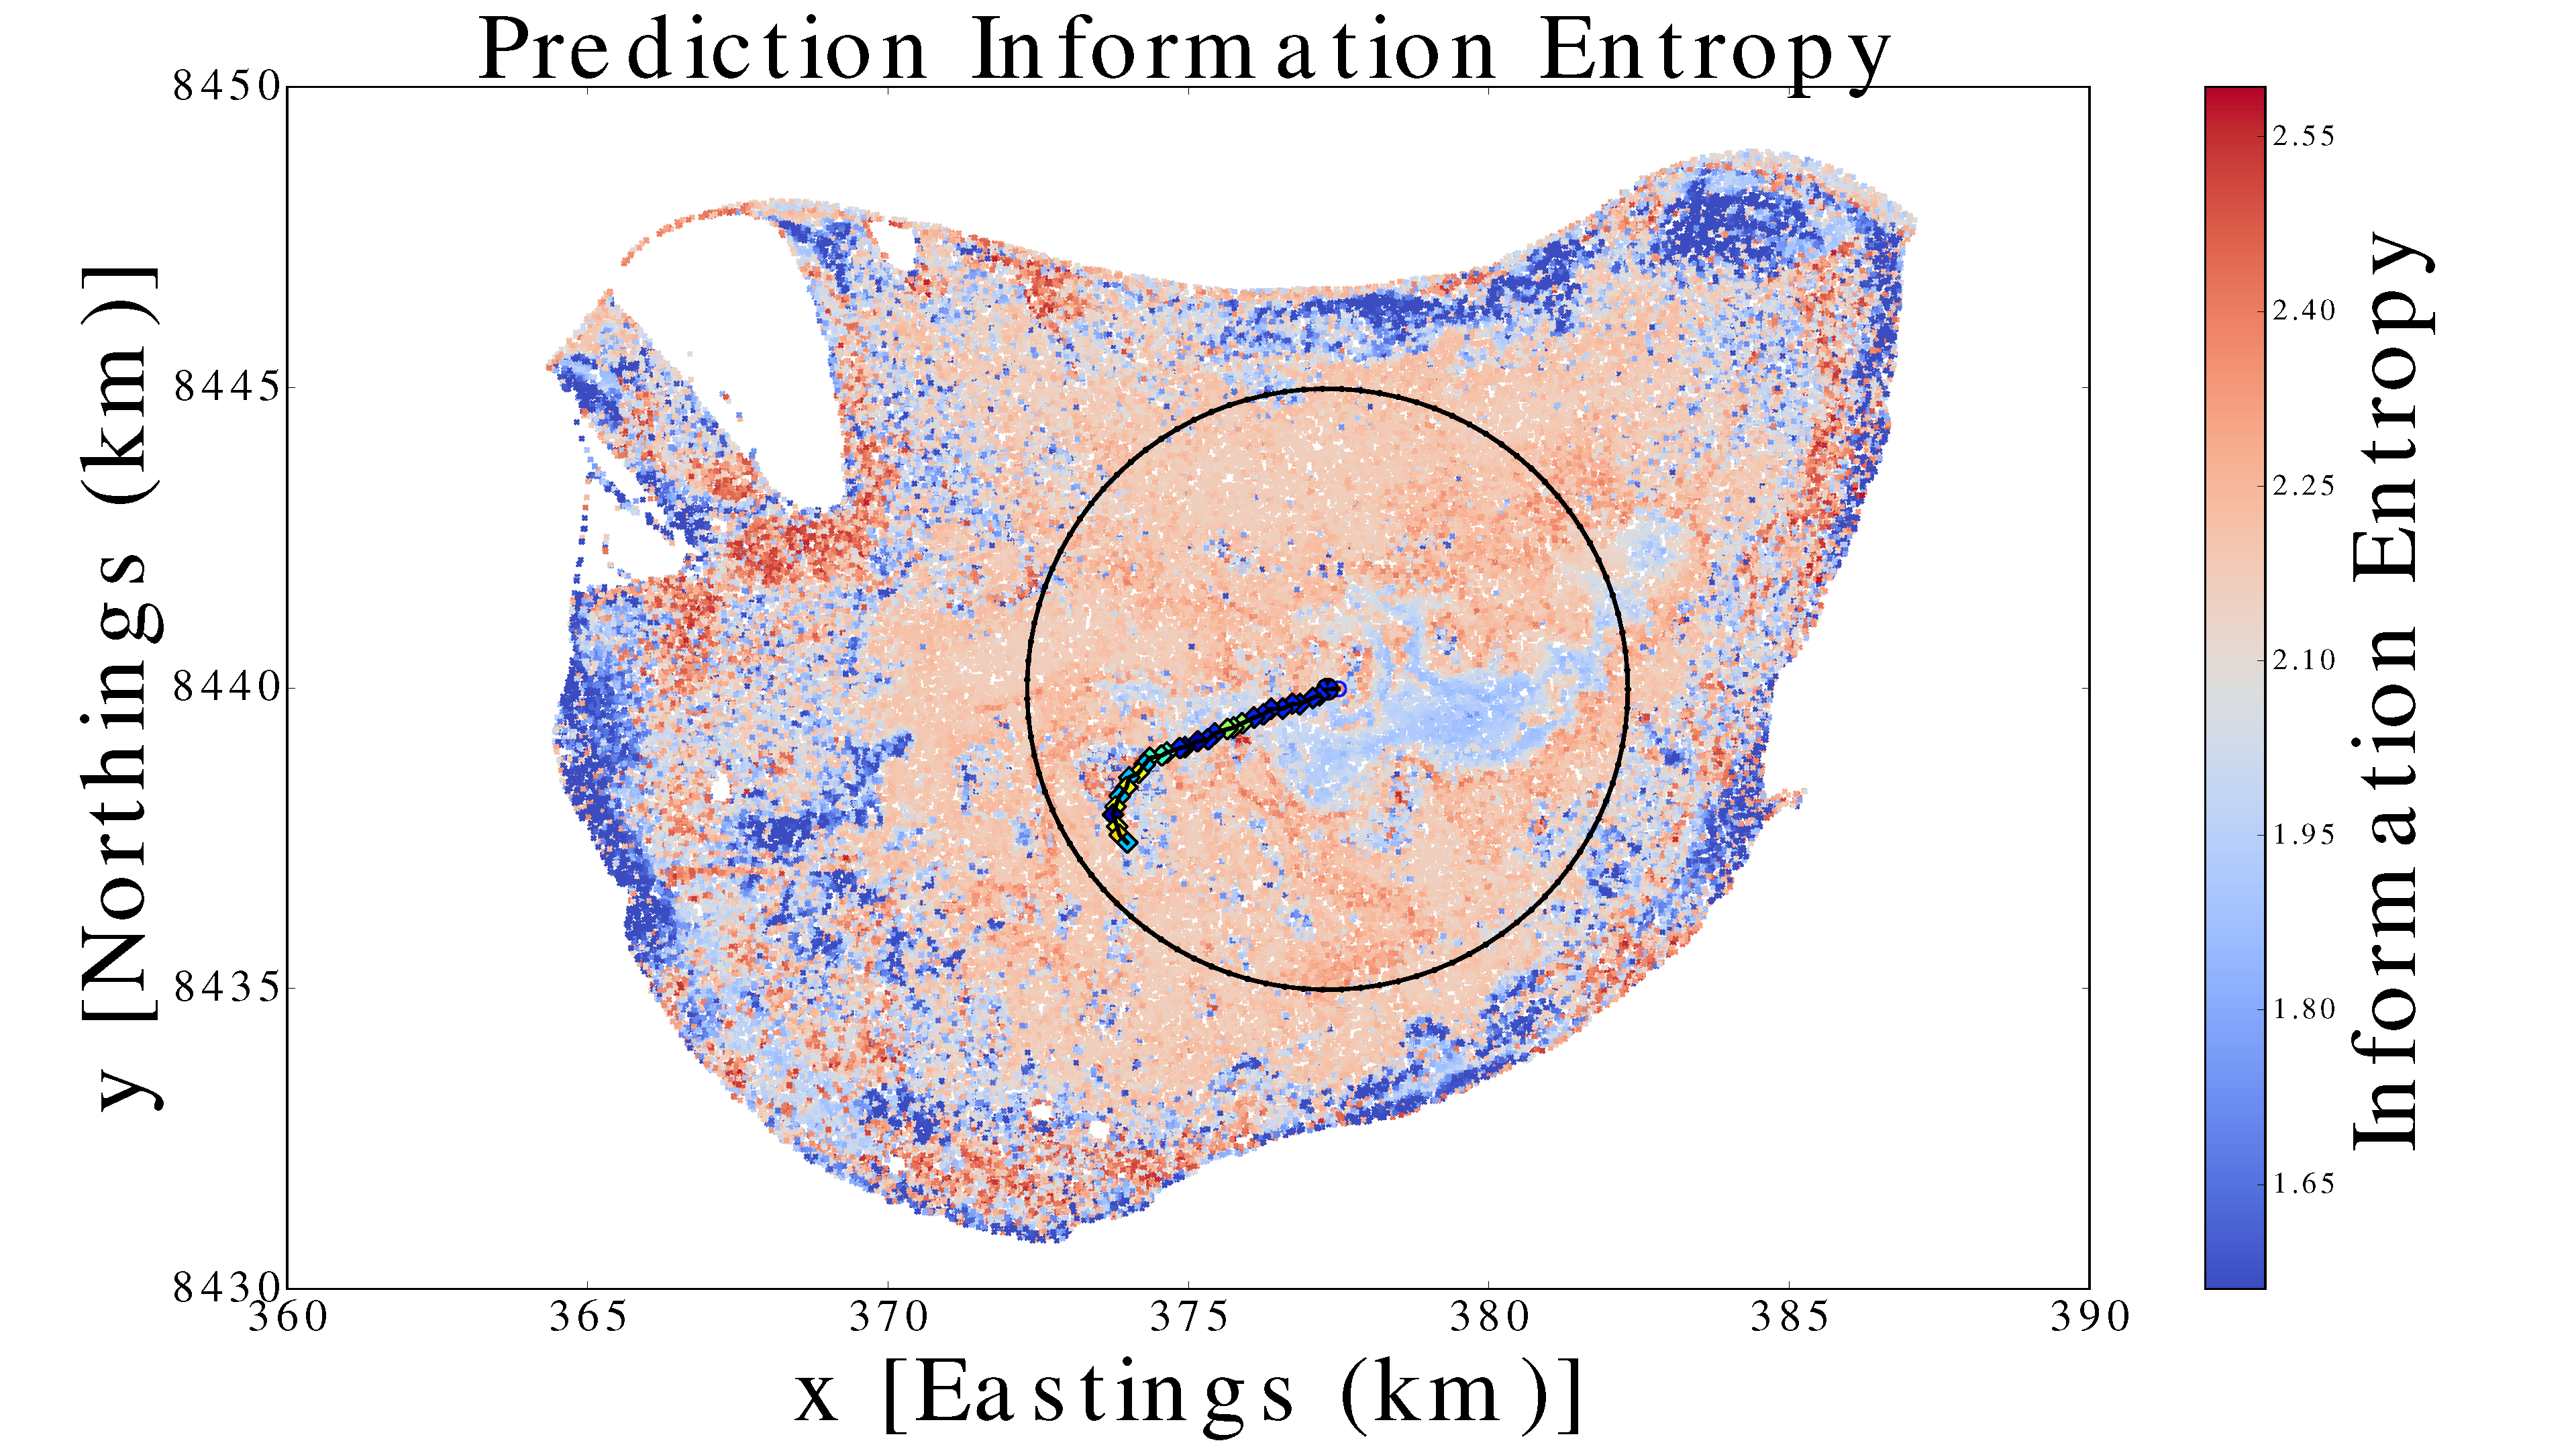
\includegraphics[width = 0.32\linewidth]{Figures/informative_seafloor_exploration/lde/mie_propose1-eps-converted-to.png}
			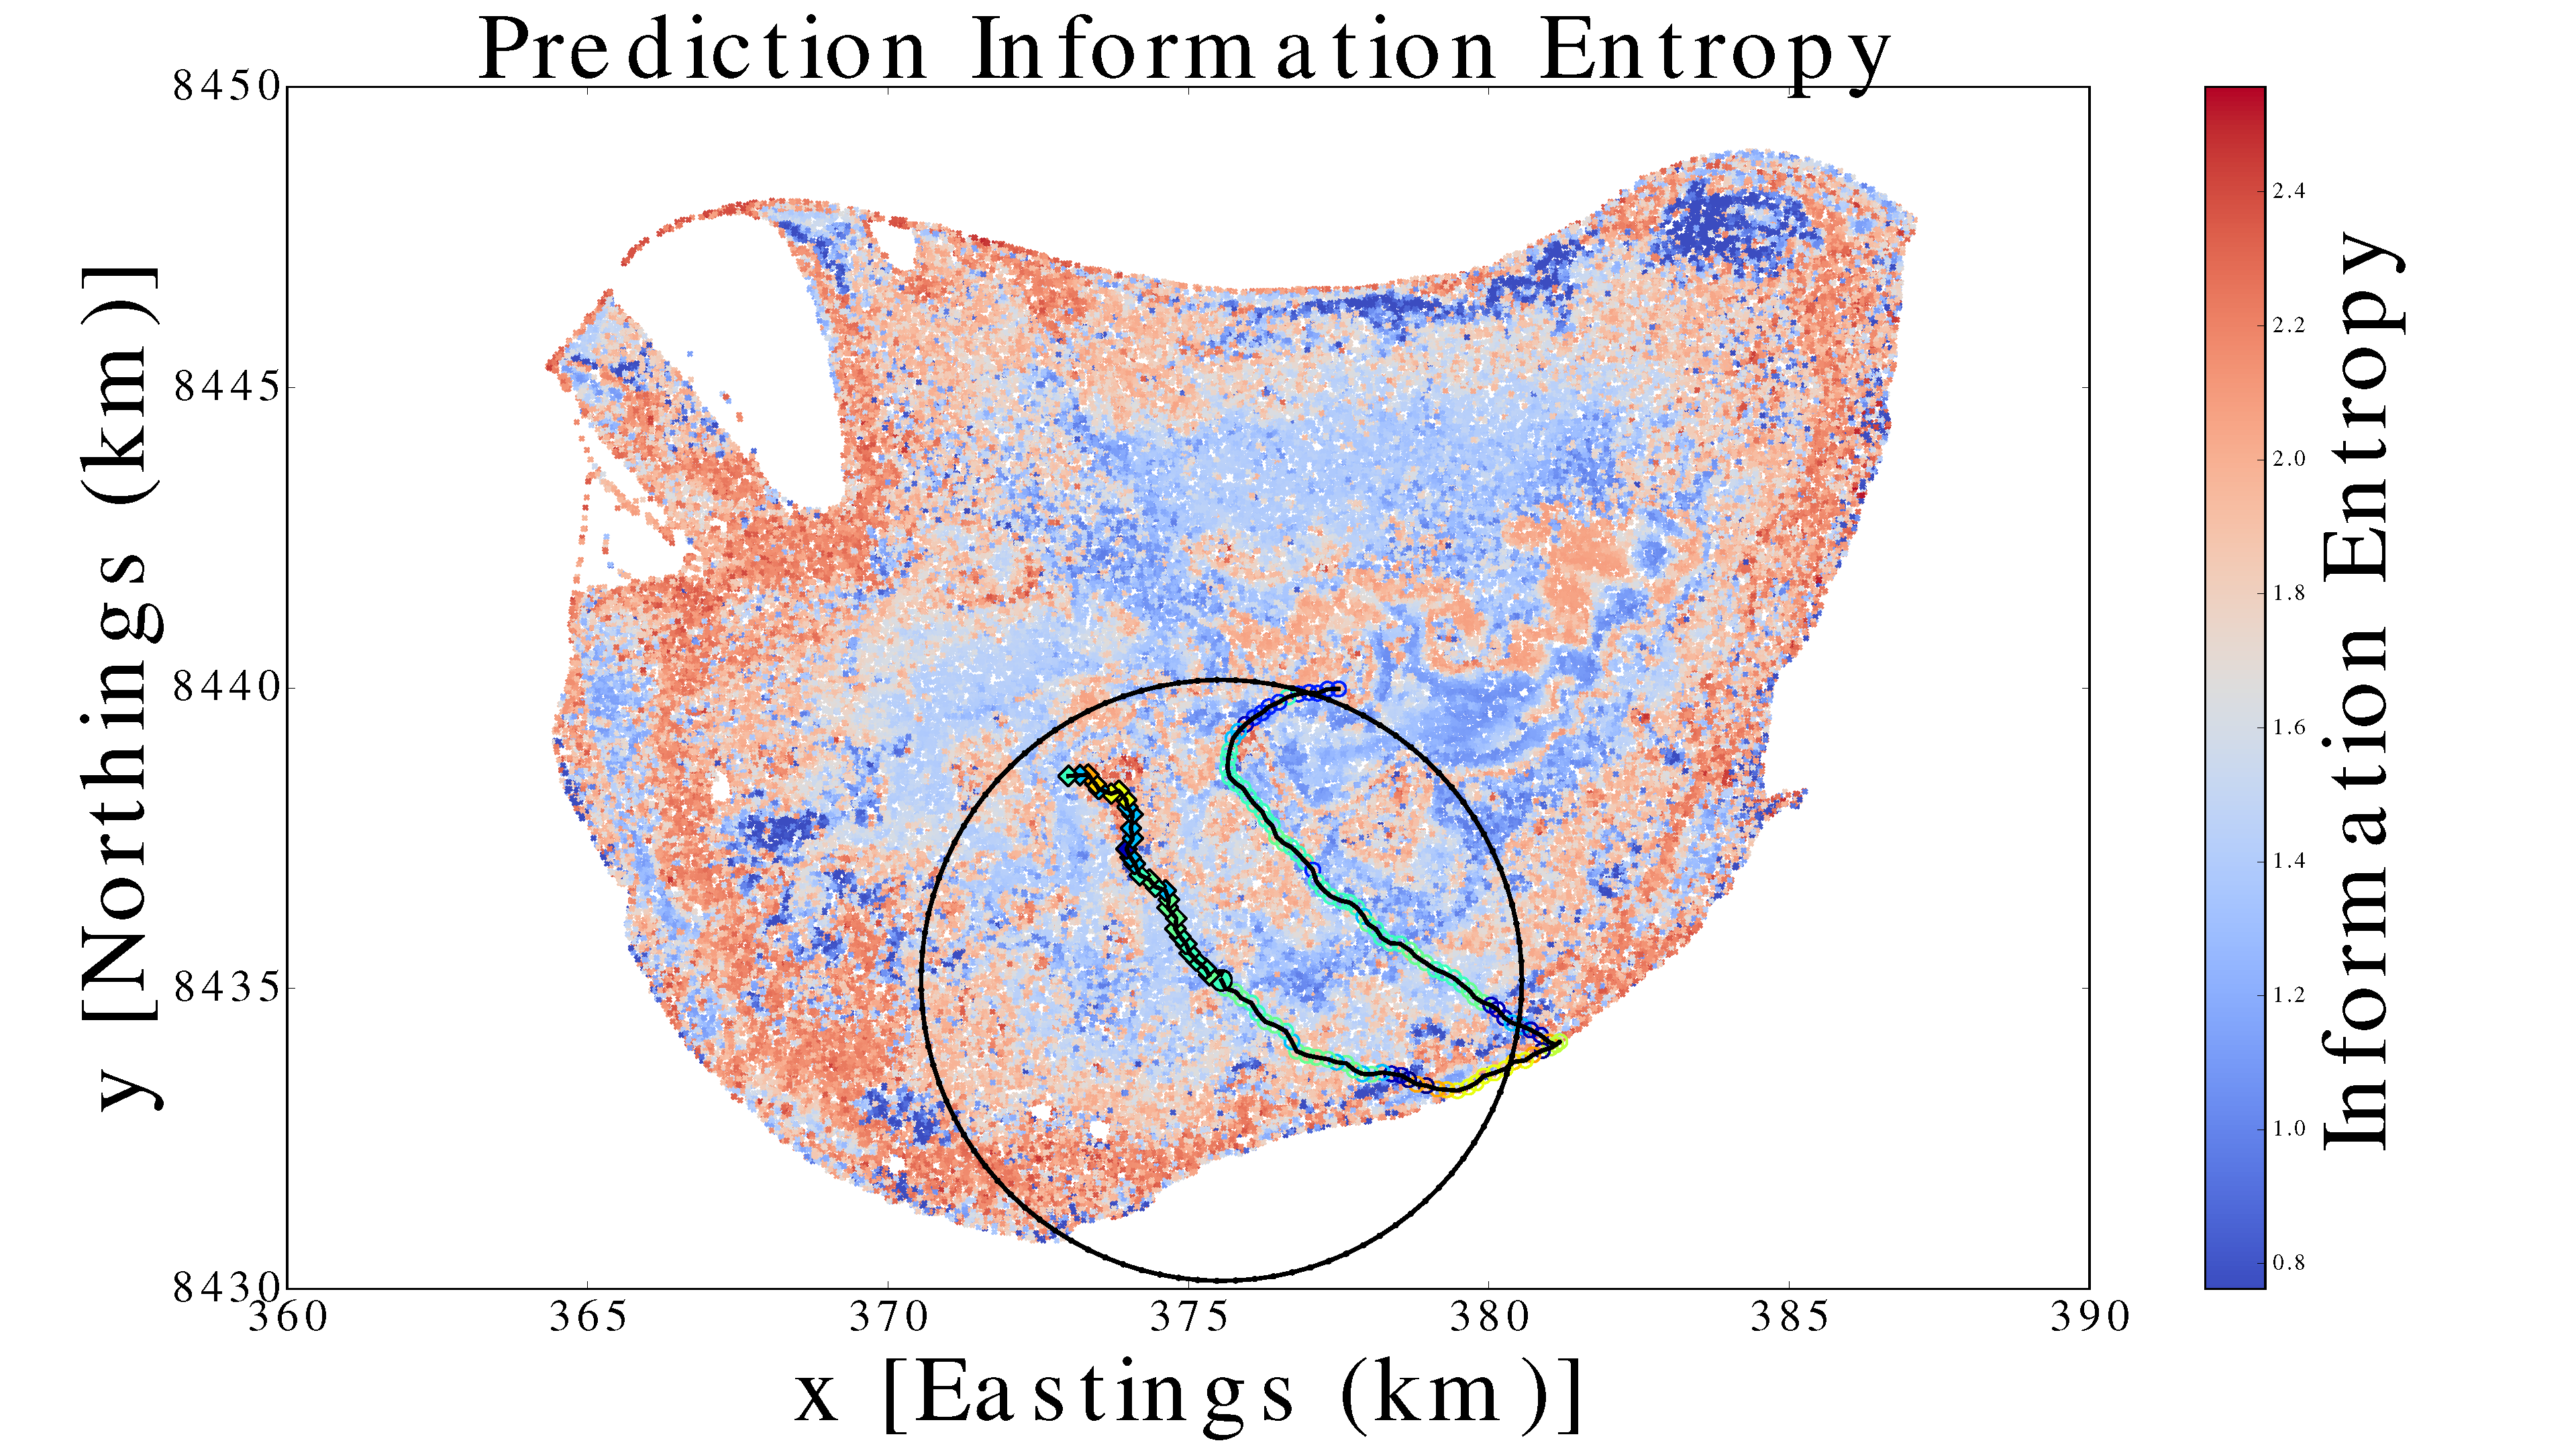
\includegraphics[width = 0.32\linewidth]{Figures/informative_seafloor_exploration/lde/mie_propose100-eps-converted-to.png}
			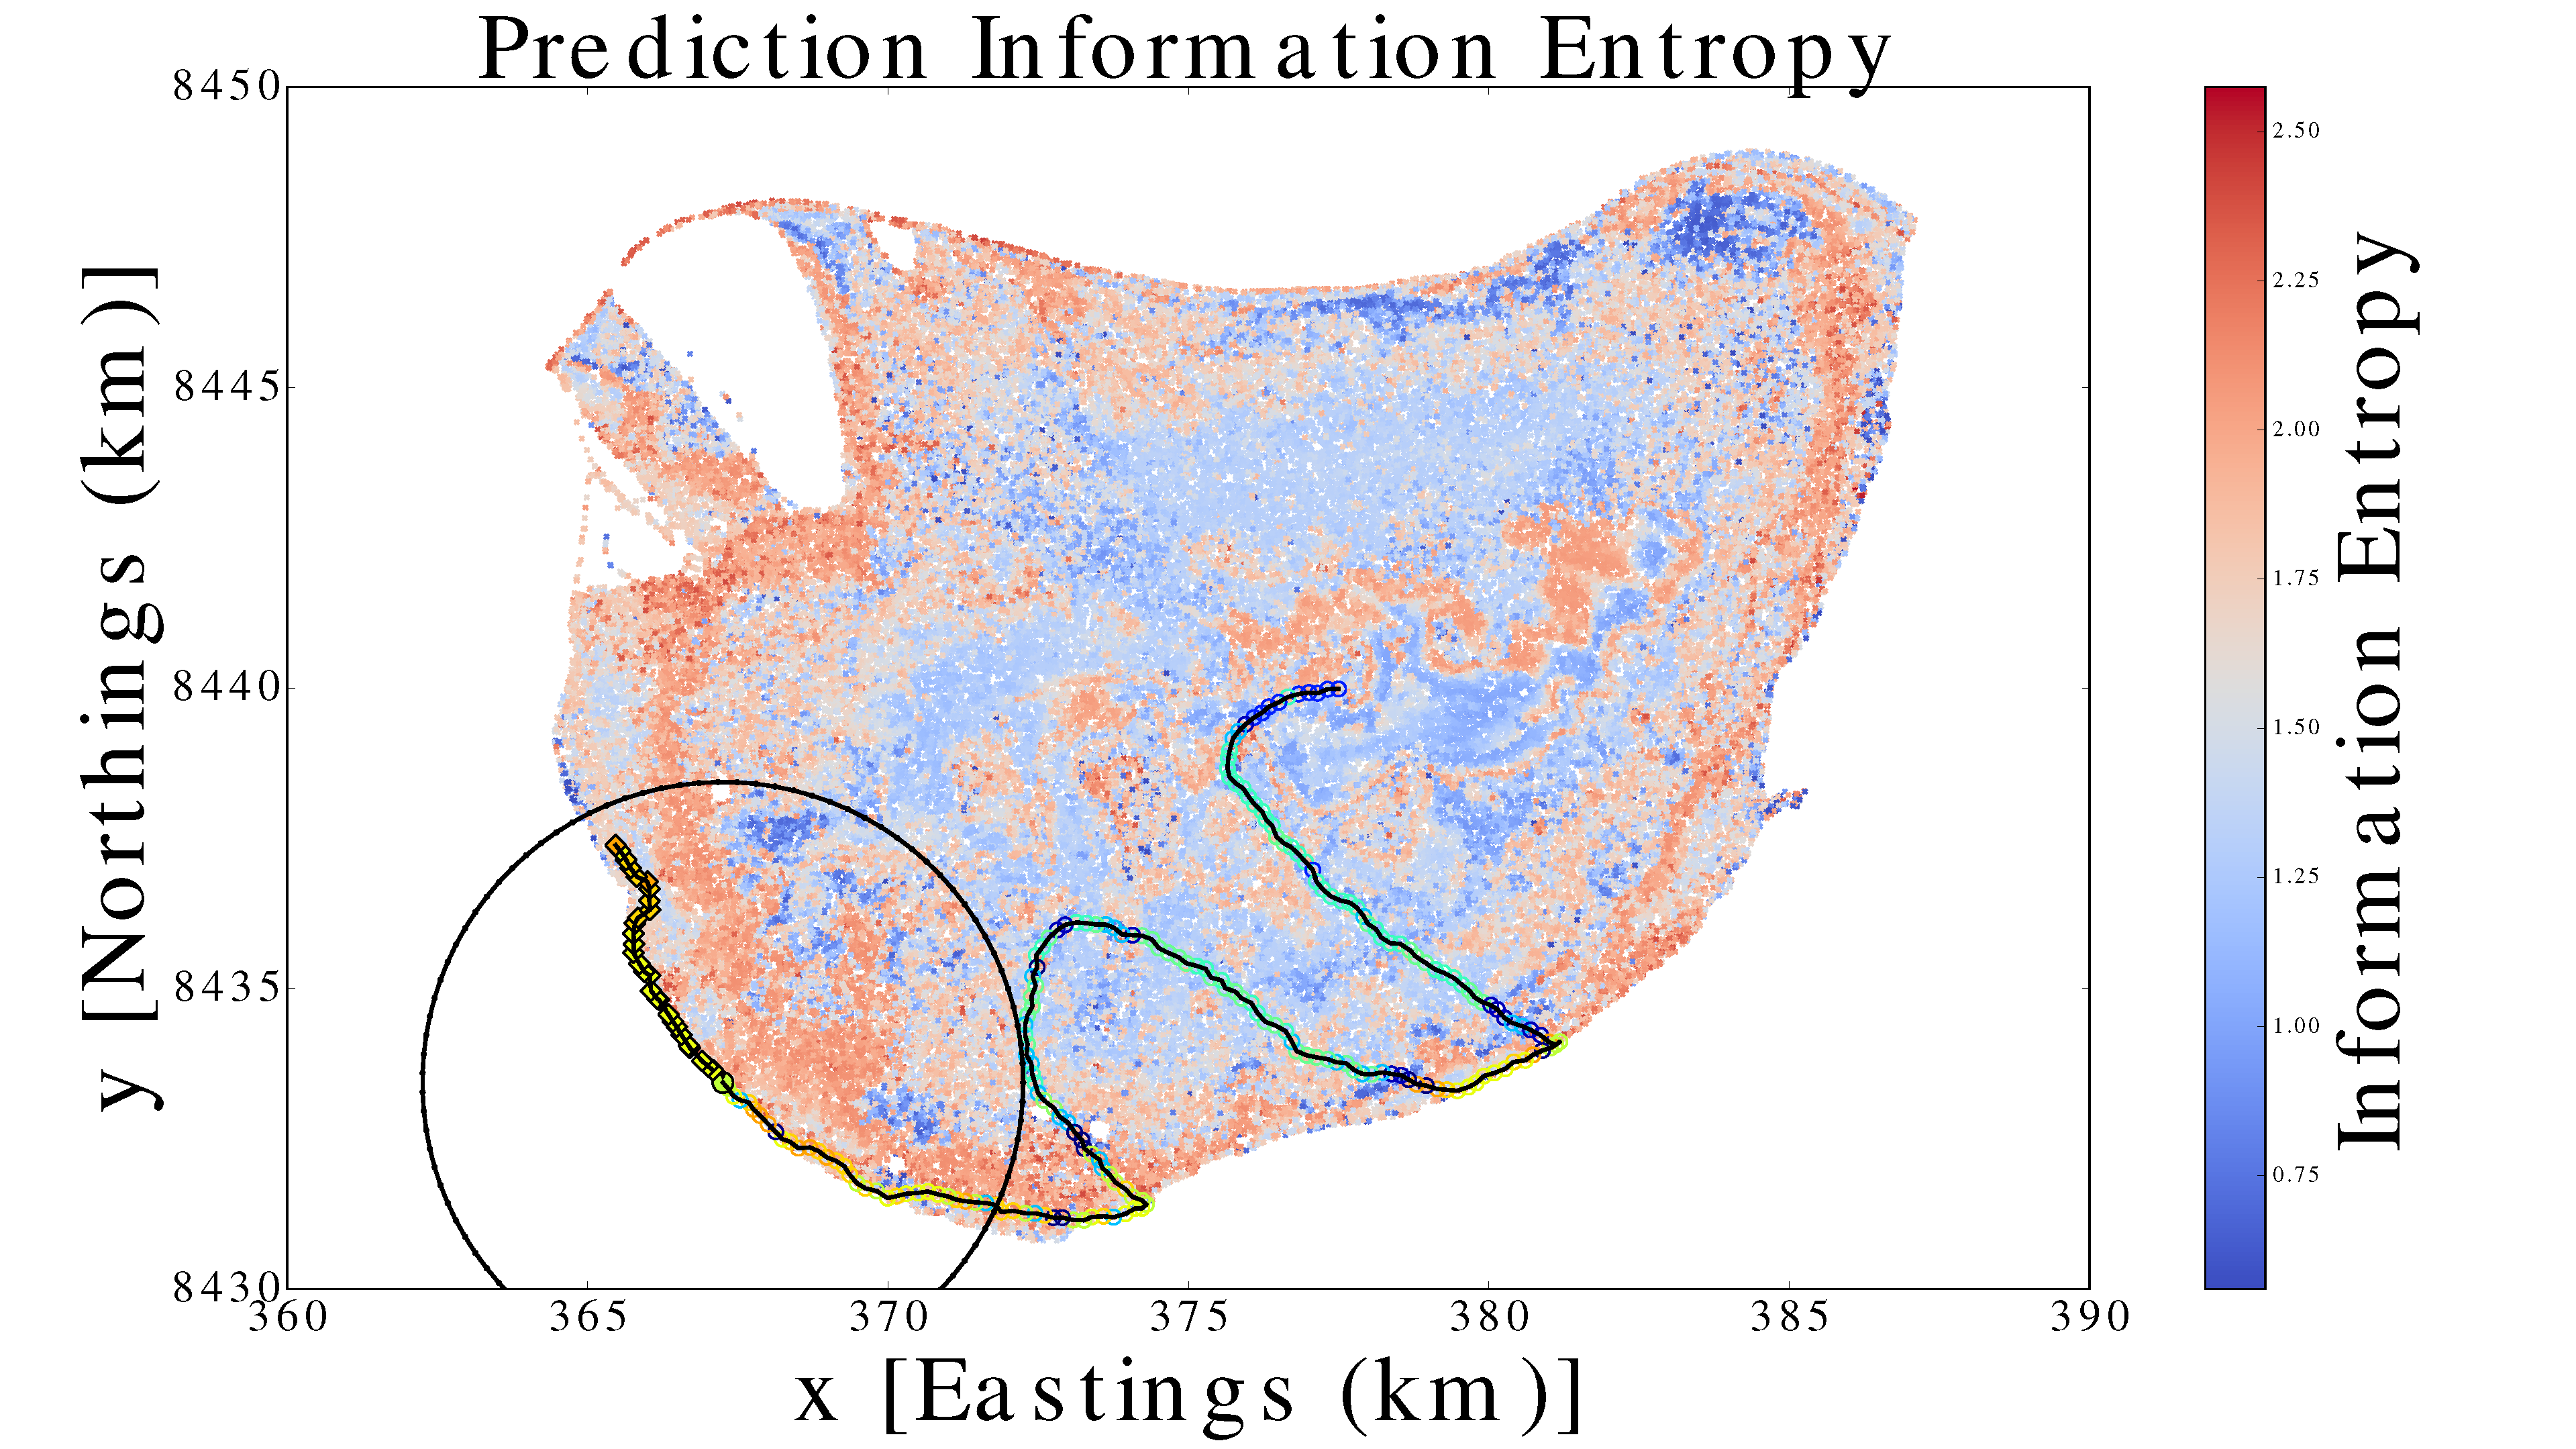
\includegraphics[width = 0.32\linewidth]{Figures/informative_seafloor_exploration/lde/mie_propose200-eps-converted-to.png}
			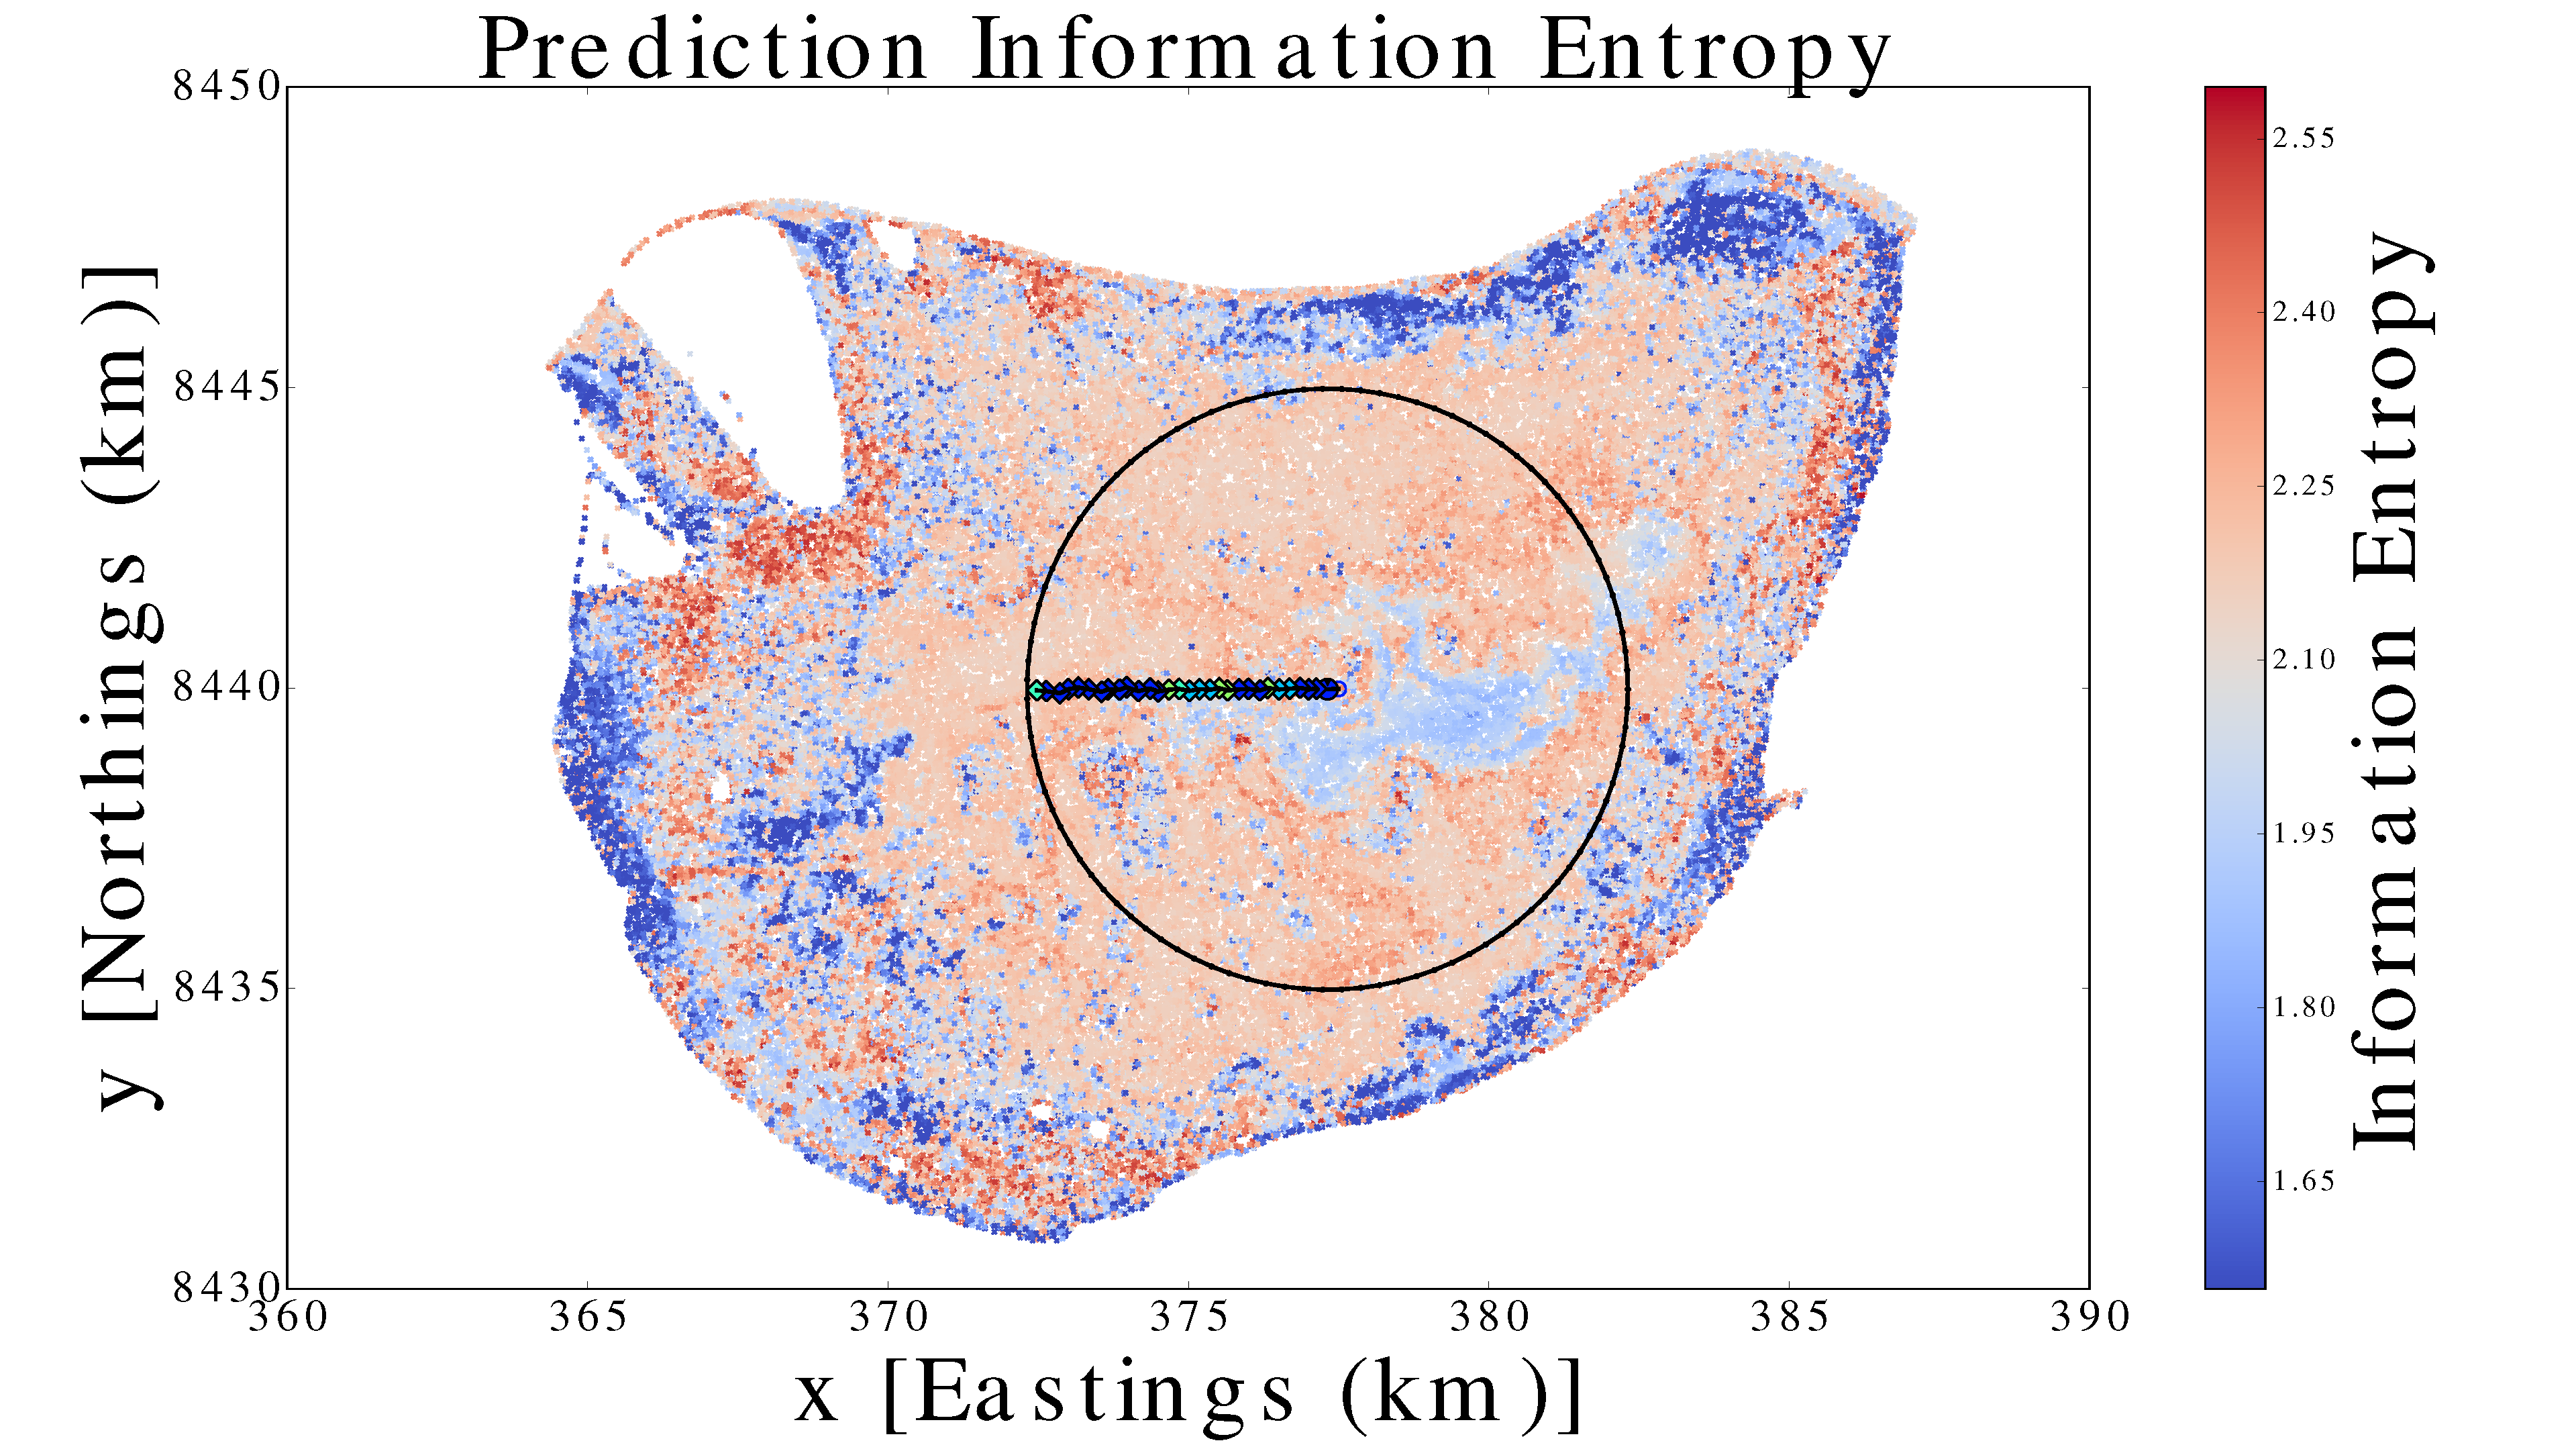
\includegraphics[width = 0.32\linewidth]{Figures/informative_seafloor_exploration/mcje/mie_propose1-eps-converted-to.png}
			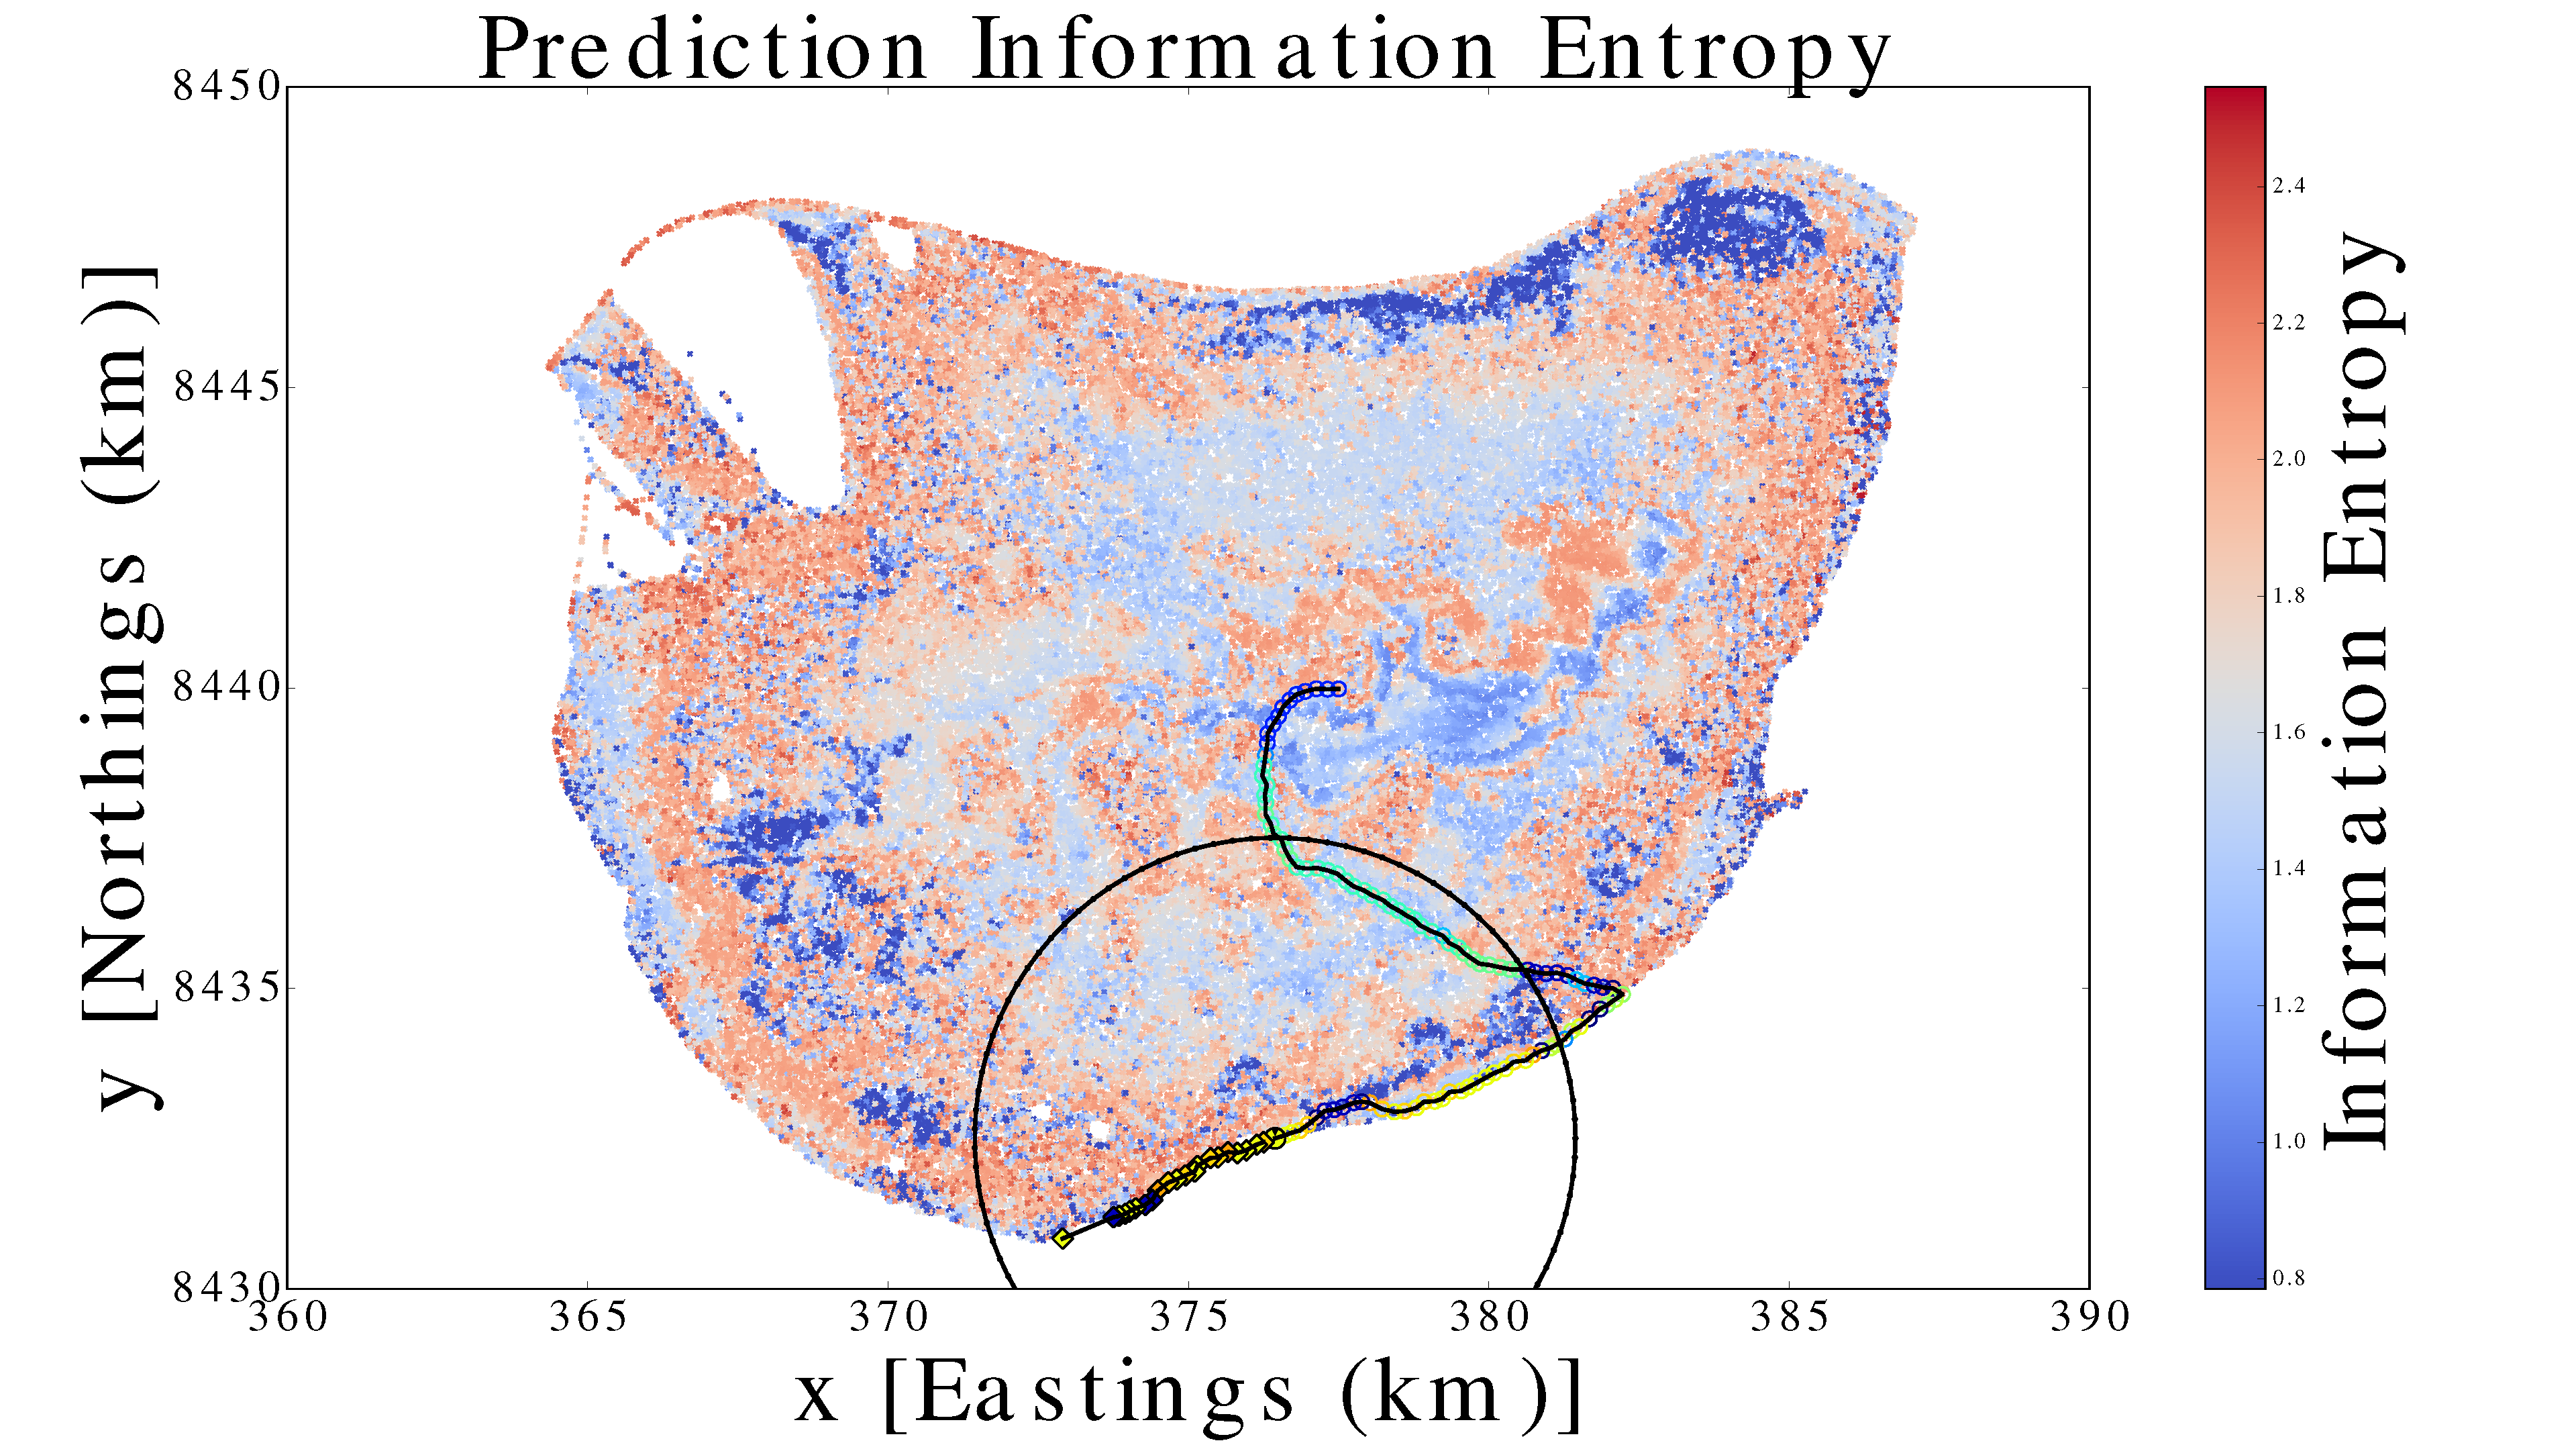
\includegraphics[width = 0.32\linewidth]{Figures/informative_seafloor_exploration/mcje/mie_propose100-eps-converted-to.png}
			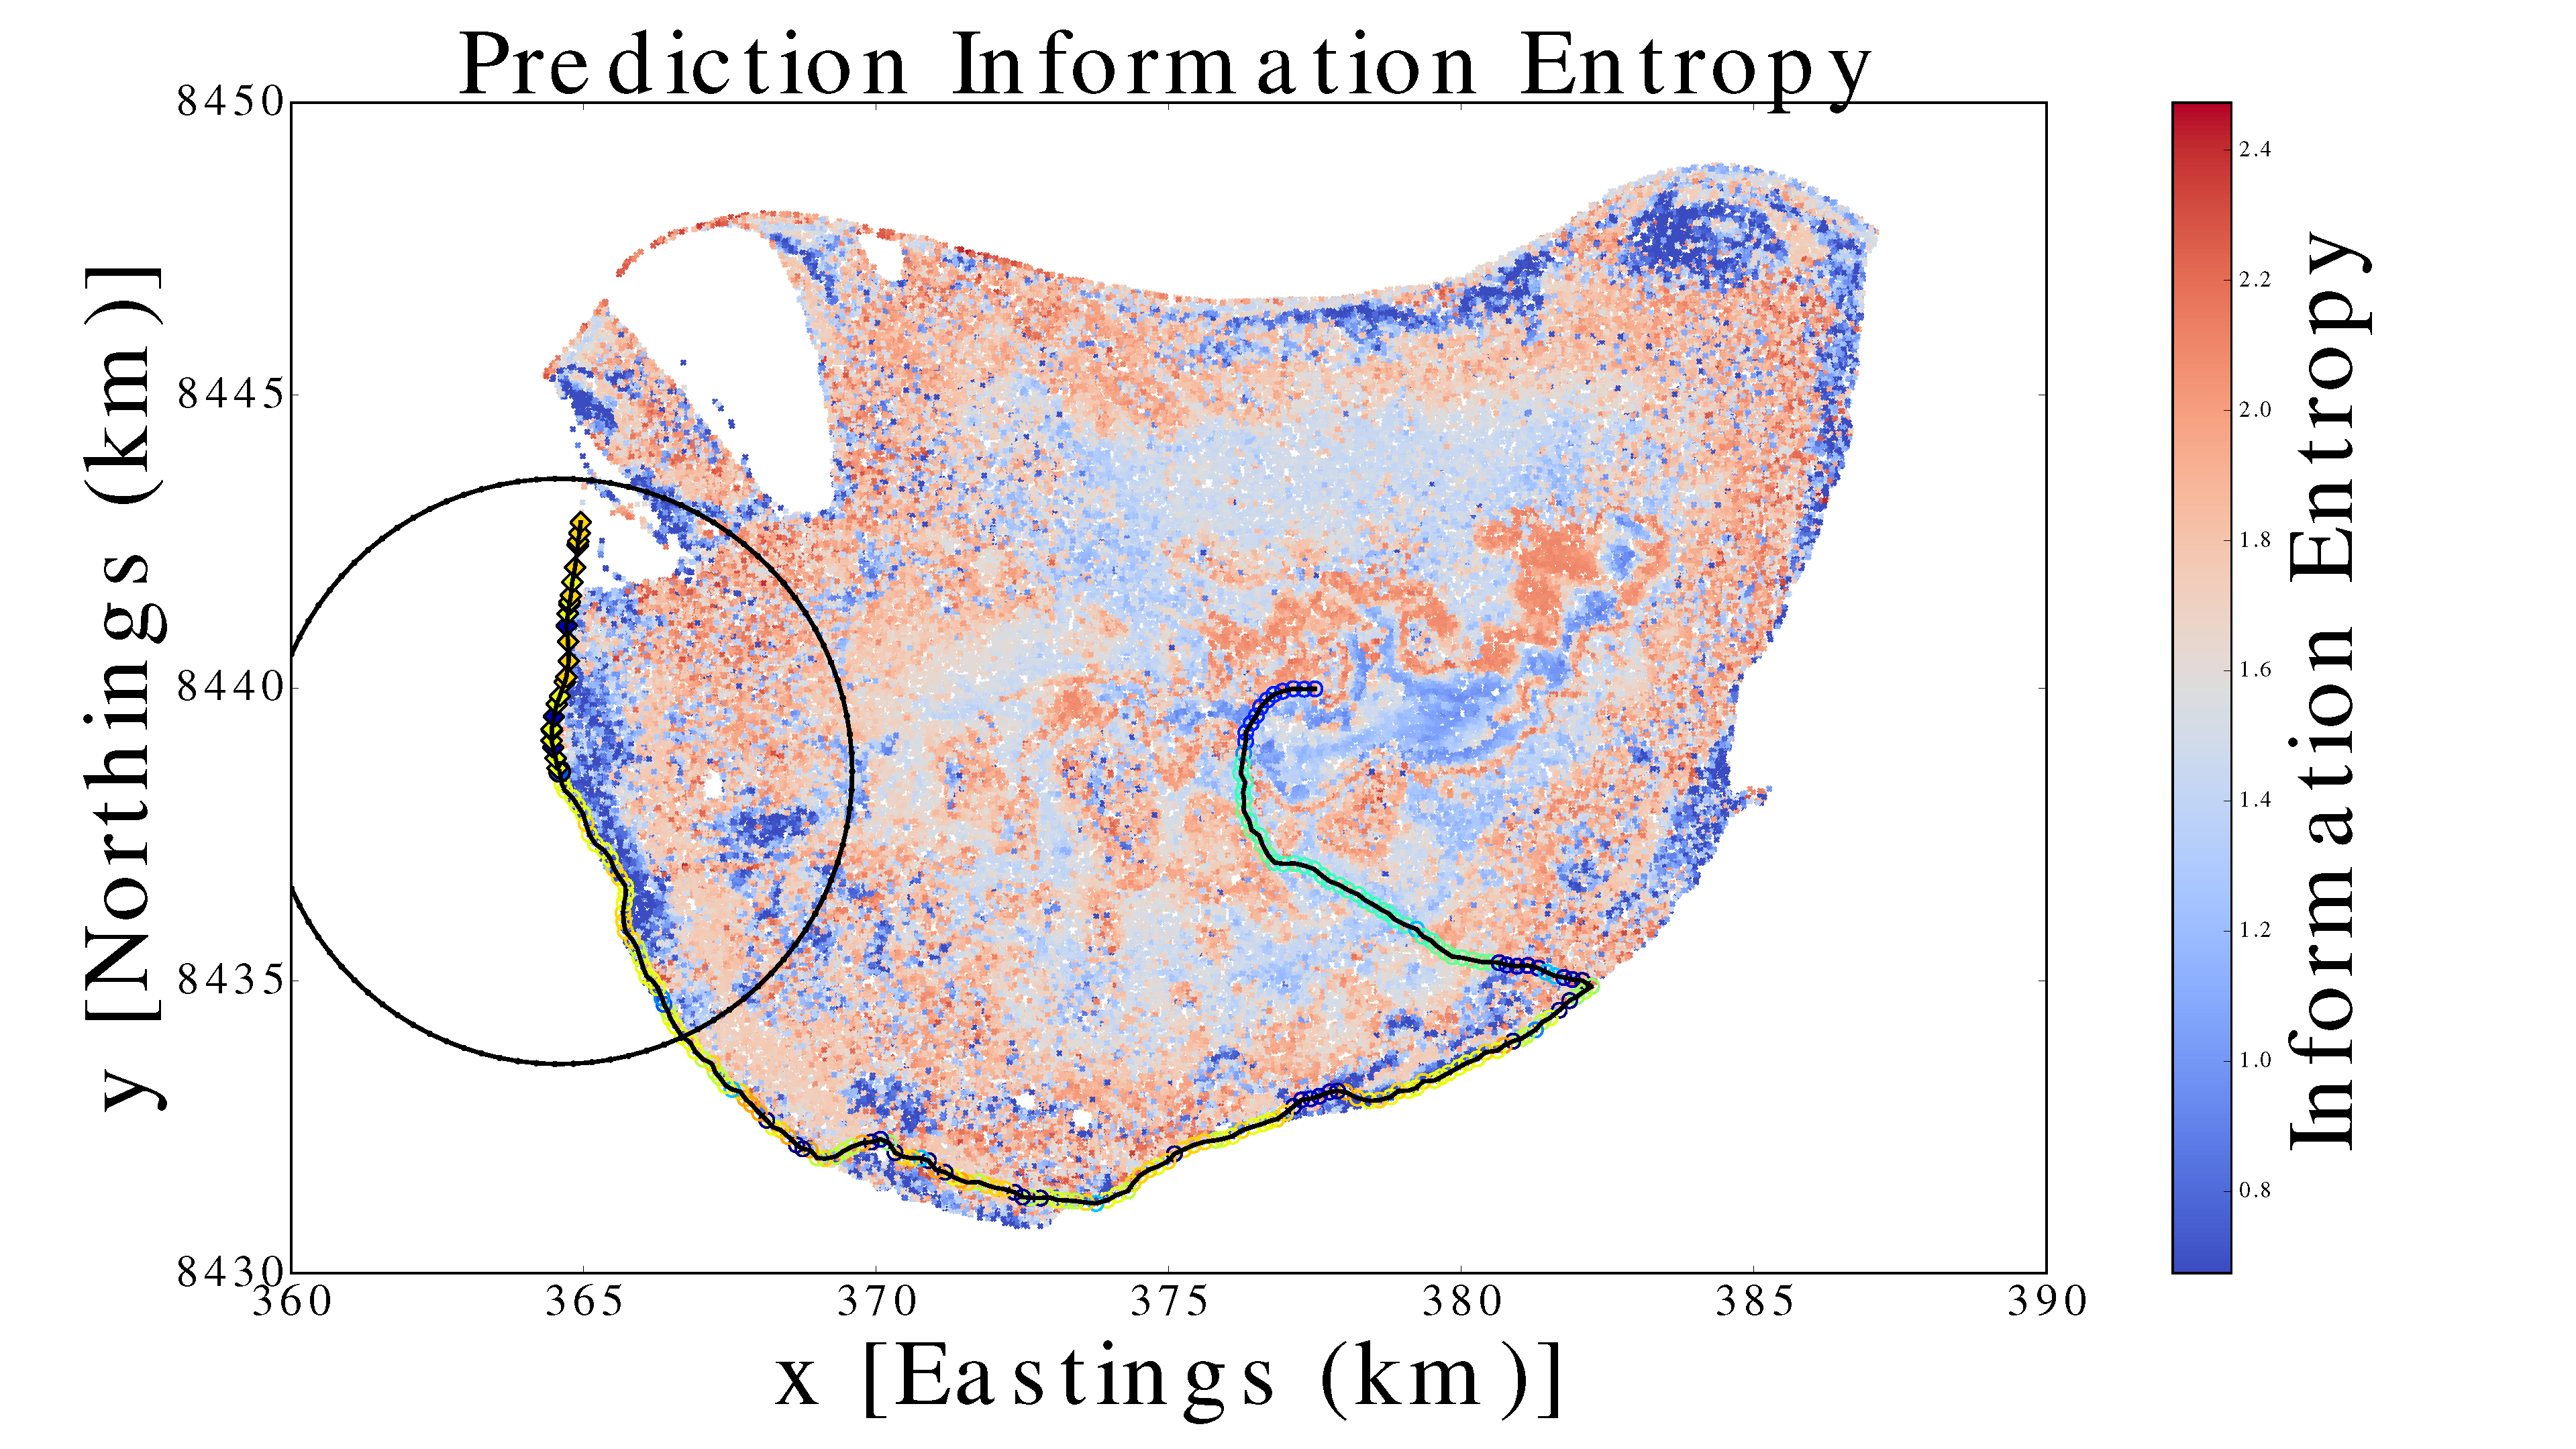
\includegraphics[width = 0.32\linewidth]{Figures/informative_seafloor_exploration/mcje/mie_propose200-eps-converted-to.png}	
		\caption{Exploration path under LDE acquisition (top) and MCJIE acquisition (bottom)}
		\label{Figure:Results:OptimalPaths}
		\end{figure*}
		
		The horizon structure selected for the Scott Reef scenario is 5 km in extent with 30 control points. Each control step is therefore $\frac{5 \mathrm{km}}{30}$ = 167 meters in length.  A comparison in performance over a distance of 33.3 km between several acquisition criterion is shown in Figure \ref{Figure:Results:CompareMethods}. Each method is tested with a horizon length of 5 km starting at two distinct initial locations - (377.5, 8440.0) and (380.0, 8440.0) km in Eastings-Northings frame. The acquisition criterion to be compared are linearised differential entropy (LDE), one step ahead information entropy (GREEDY), random walk (RANDOM), Monte Carlo estimated joint information entropy (MCJIE), mean of marginalised information entropy (MIE), predetermined spiral path (FIXED-SPIRAL), and predetermined line segmented paths (FIXED-LINES). Of these, only LDE and MCJIE acquisitions consider mutual information.

%('Location 1 with LDE', 0.16442000000000001)
%('Location 1 with LINES', 0.20402000000000001)
%('Location 1 with MCJIE', 0.22992000000000001)
%('Location 1 with MIE', 0.32114999999999999)
%('Location 1 with SPIRAL', 0.33735999999999999)
%('Location 1 with RANDOM', 0.34873999999999999)
%('Location 1 with GREEDY', 0.42856)
%----------
%('Location 2 with LDE', 0.20383999999999999)
%('Location 2 with LINES', 0.25052000000000002)
%('Location 2 with MCJIE', 0.27012000000000003)
%('Location 2 with RANDOM', 0.35681000000000002)
%('Location 2 with GREEDY', 0.37630000000000002)
%('Location 2 with MIE', 0.40111999999999998)
%('Location 2 with SPIRAL', 0.43160999999999999)
		  				
		There are several measures of performance criterion that can be used to measure performance. As the aim is to reduce misclassification rate, we compare the percentage of prediction misses between each method. Each method begins with the same scenario, for which the initial misclassification rate with 200 training points is 41.54\% (figure \ref{Figure:Results:ScottReefInitialPredictions}). From table \ref{Table:Results:CompareMethods}, we see that under this performance criterion, the LDE method performs the best, with a final misclassification rate of 16.44\% and 20.38\% for location 1 and 2 respectively at the end of the journey. Methods FIXED-LINES (20.40\% and 25.05\%) and MCJIE (22.29\% and 27.01\%) follow in performance. The predetermined line segmented paths (FIXED-LINES) are hand-picked by subjective judgement from after-the-fact knowledge, and serve as an intuitive anchor for comparison. Notice that because the LDE method prioritises on decision boundaries, it achieves a lower misclassification rate through appropriately reducing both bias and variance at decision boundaries.
	
		\begin{figure}[!htbp]
		\centering
			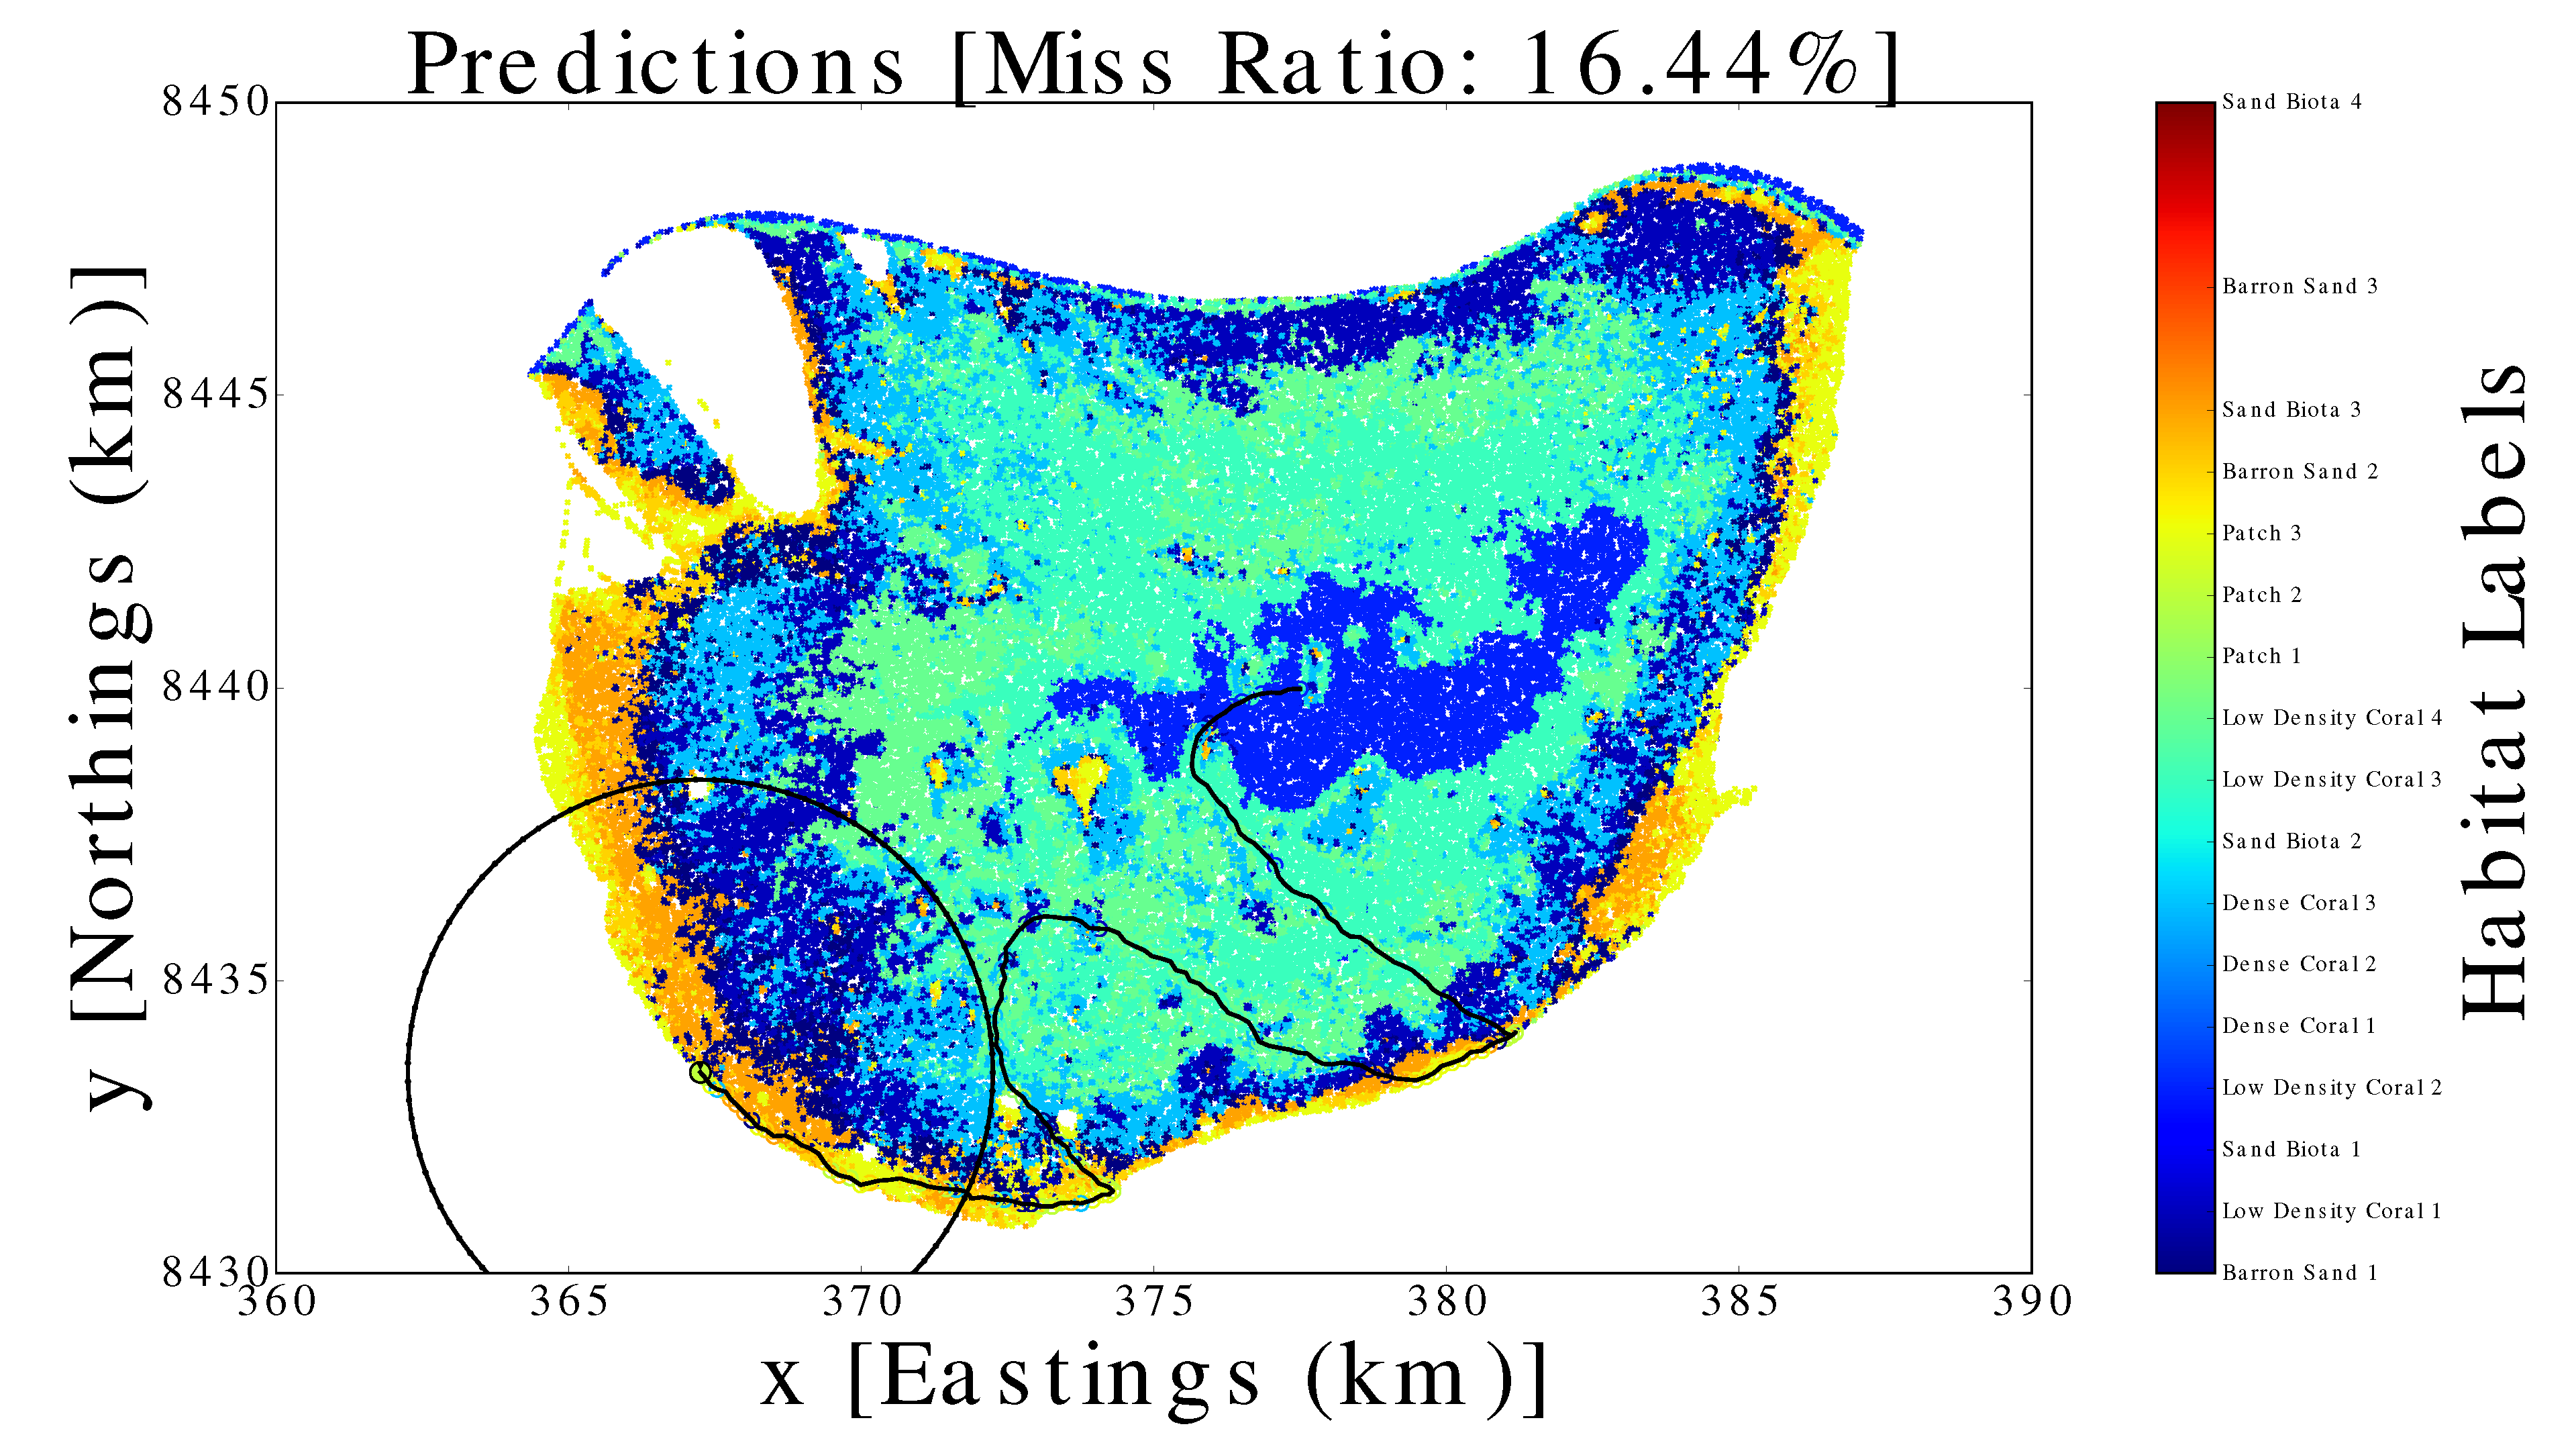
\includegraphics[width = \linewidth]{Figures/informative_seafloor_exploration/lde/pred200-eps-converted-to.png}
		\caption{Final Predictions}
		\label{Figure:Results:FinalPredictions}
		\end{figure}
				
		Figures \ref{Figure:Results:OptimalPaths} show snapshots of the resulting path under LDE and MCJIE acquisition respectively, layered onto the prediction information entropy map. The snapshots are taken at 0.17 km, 16.67 km, and 33.33 km into the journey. Figure \ref{Figure:Results:FinalPredictions} shows the final predictions after 33.33 km under LDE acquisition. The circle represents the horizon length for which the vehicle considers in at each time step, with the vehicle at the center. The path with empty circles represent the path it has taken, and the path with filled hexagons extending from the current location represent the immediate proposed path from the receding horizon optimisation.
		
		As we expect, the paths from the two methods are similar, with LDE acquisition achieving a misclassification ratio of approximately 4\% less. This difference is visible through the lower amount of information entropy around the inner regions of the reef under LDE acquisition compared to MCJIE acquisition. Unlike other methods, both the LDE and MCJIE method take into consideration the mutual information of the proposed path, so that both methods outperform myopic or open loop methods (figure \ref{Figure:Results:CompareMethods}). In the figure shown, the Monte Carlo approach uses 1000 sample draws from the GP classifier to estimate the joint distribution for 30 control points, and experiences little improvement under misclassification criterion with more samples. This results demonstrates that under a receding horizon formulation, using LDE acquisition achieves lower misclassification rate on average than other acquisition functions - most importantly MCJIE acquisition. Furthermore, a receding horizon method achieves lower misclassification rate than myopic approaches under the same acquisition function.	

		\begin{table*}[t]
			\begin{center}
				\begin{tabular}{ |c||c|c|c|c|c|c|c| }
				\hline
				Method & LDE & MCJIE & MIE & GREEDY & RANDOM & FIXED - LINES & FIXED - SPIRAL \\
				\hline
				Location 1 & 16.44 & 22.99 & 32.11 & 43.86 & 34.87 & 20.40 & 33.74 \\
				Location 2 & 20.38 & 27.01 & 40.11 & 37.63 & 35.68 & 25.05 & 43.16 \\
				\hline
				\end{tabular}
			\end{center}
	  	\caption{Comparison of final misclassification rate (\%) between informative exploration methods}
	  	\label{Table:Results:CompareMethods}			
	  	\end{table*}	
	  	
		\begin{figure}[!htbp]
		\centering
			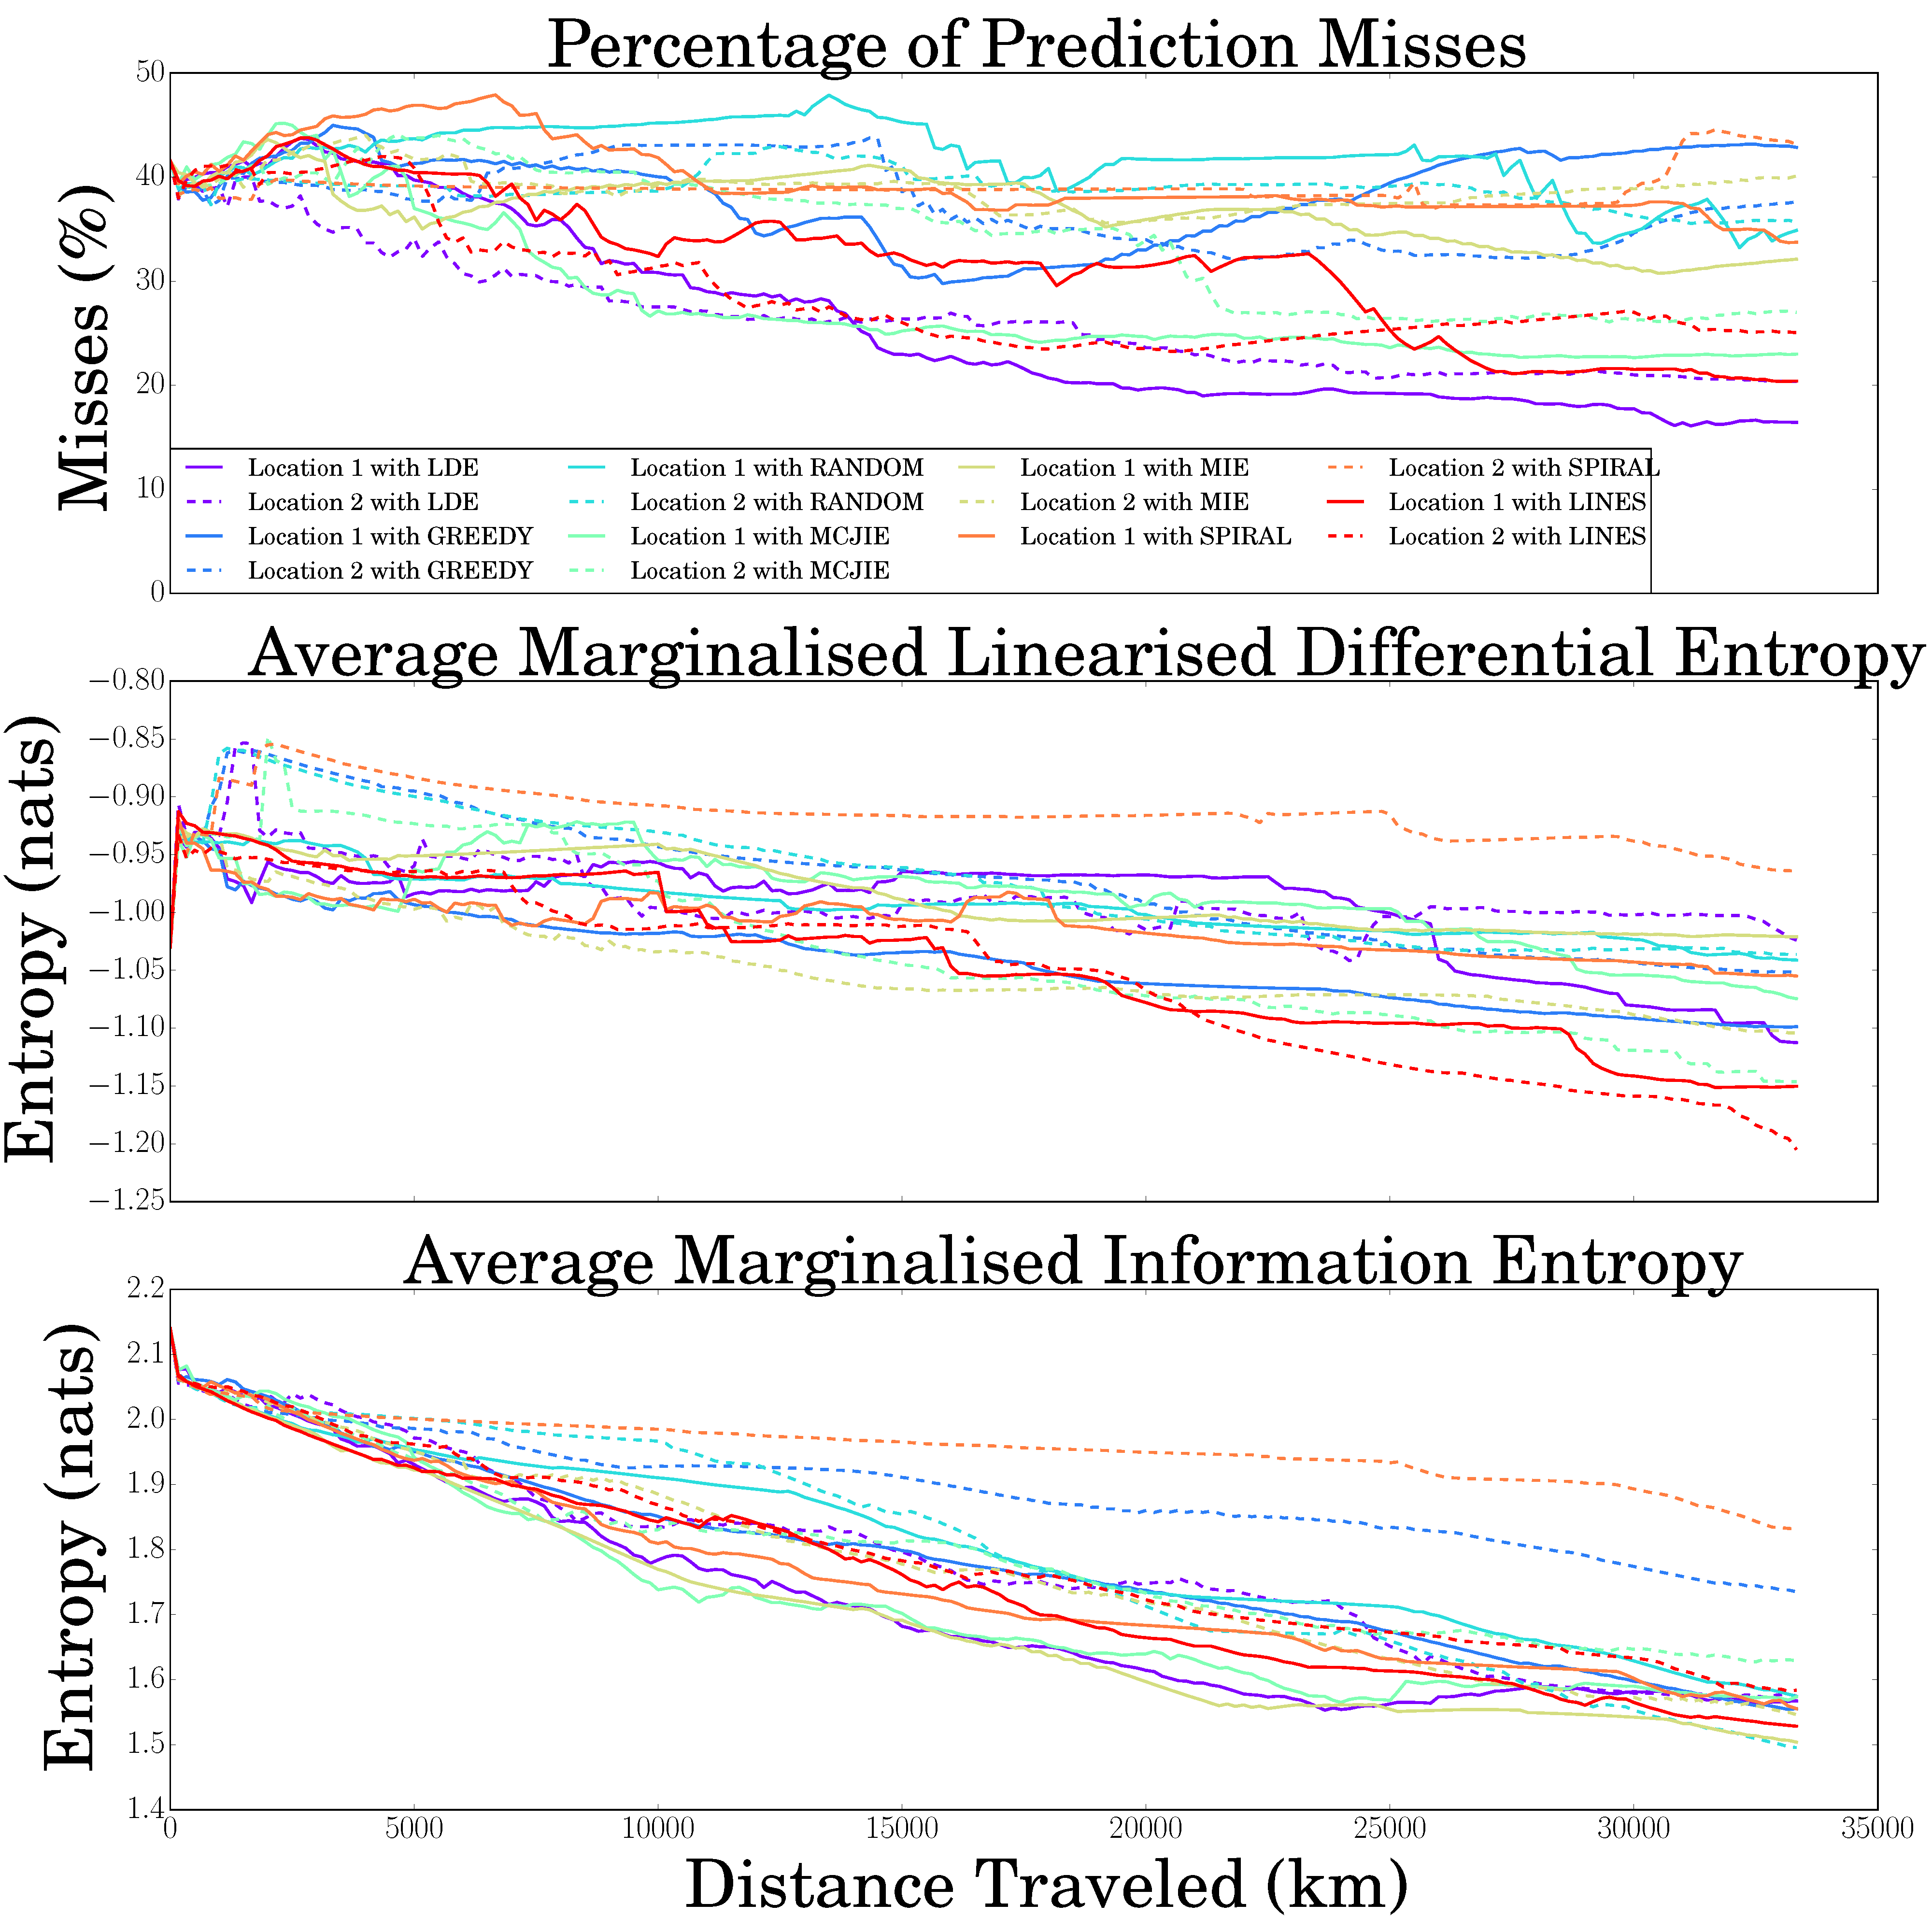
\includegraphics[width = \linewidth]{Figures/compare_methods-eps-converted-to.png}
		\caption{Comparison of informative exploration methods}
		\label{Figure:Results:CompareMethods}
		\end{figure}
		
%		\begin{figure}[!htbp]
%		\centering
%			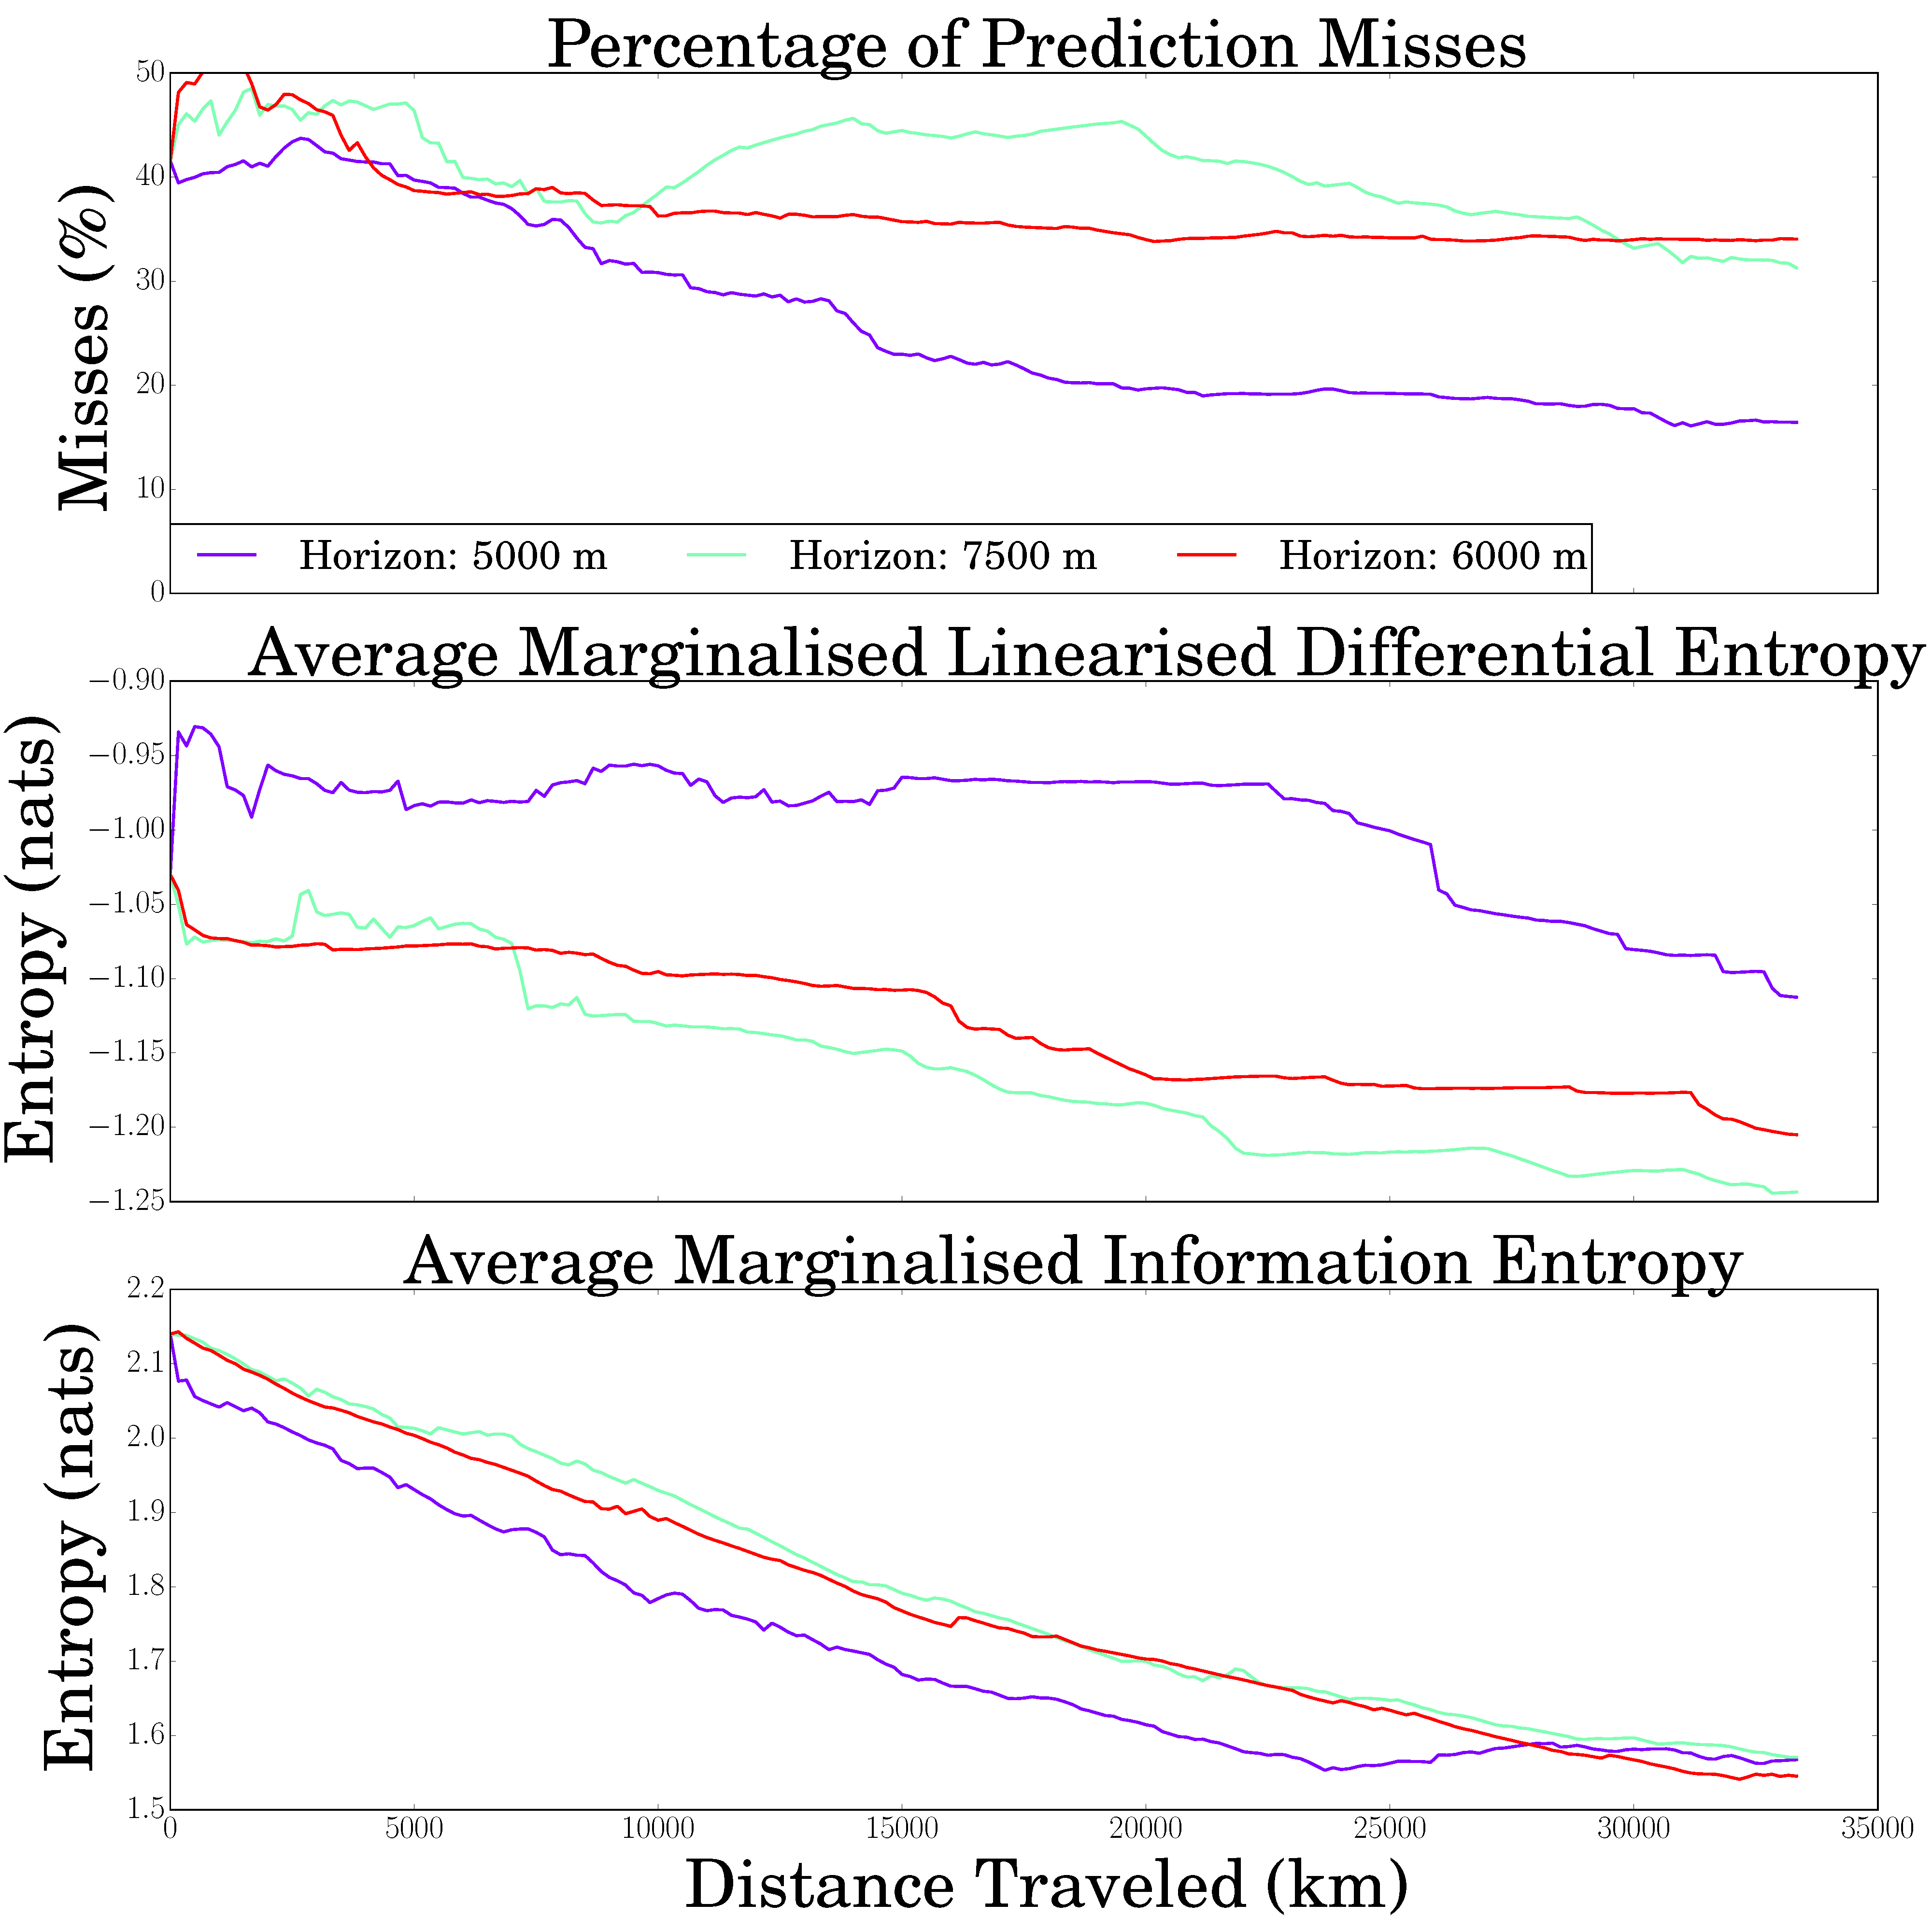
\includegraphics[width = \linewidth]{Figures/compare_horizons-eps-converted-to.png}
%		\caption{Variability over horizon lengths}
%		\label{Figure:Results:CompareHorizons}
%		\end{figure}
%	
%		In figures \ref{Figure:Results:CompareHorizons} and \ref{Figure:Results:CompareLocations} we show the stability and consistency of the approach under varying horizon lengths and starting locations for the case of Scott Reef. 
%		
%		\begin{figure}[!htbp]
%		\centering
%			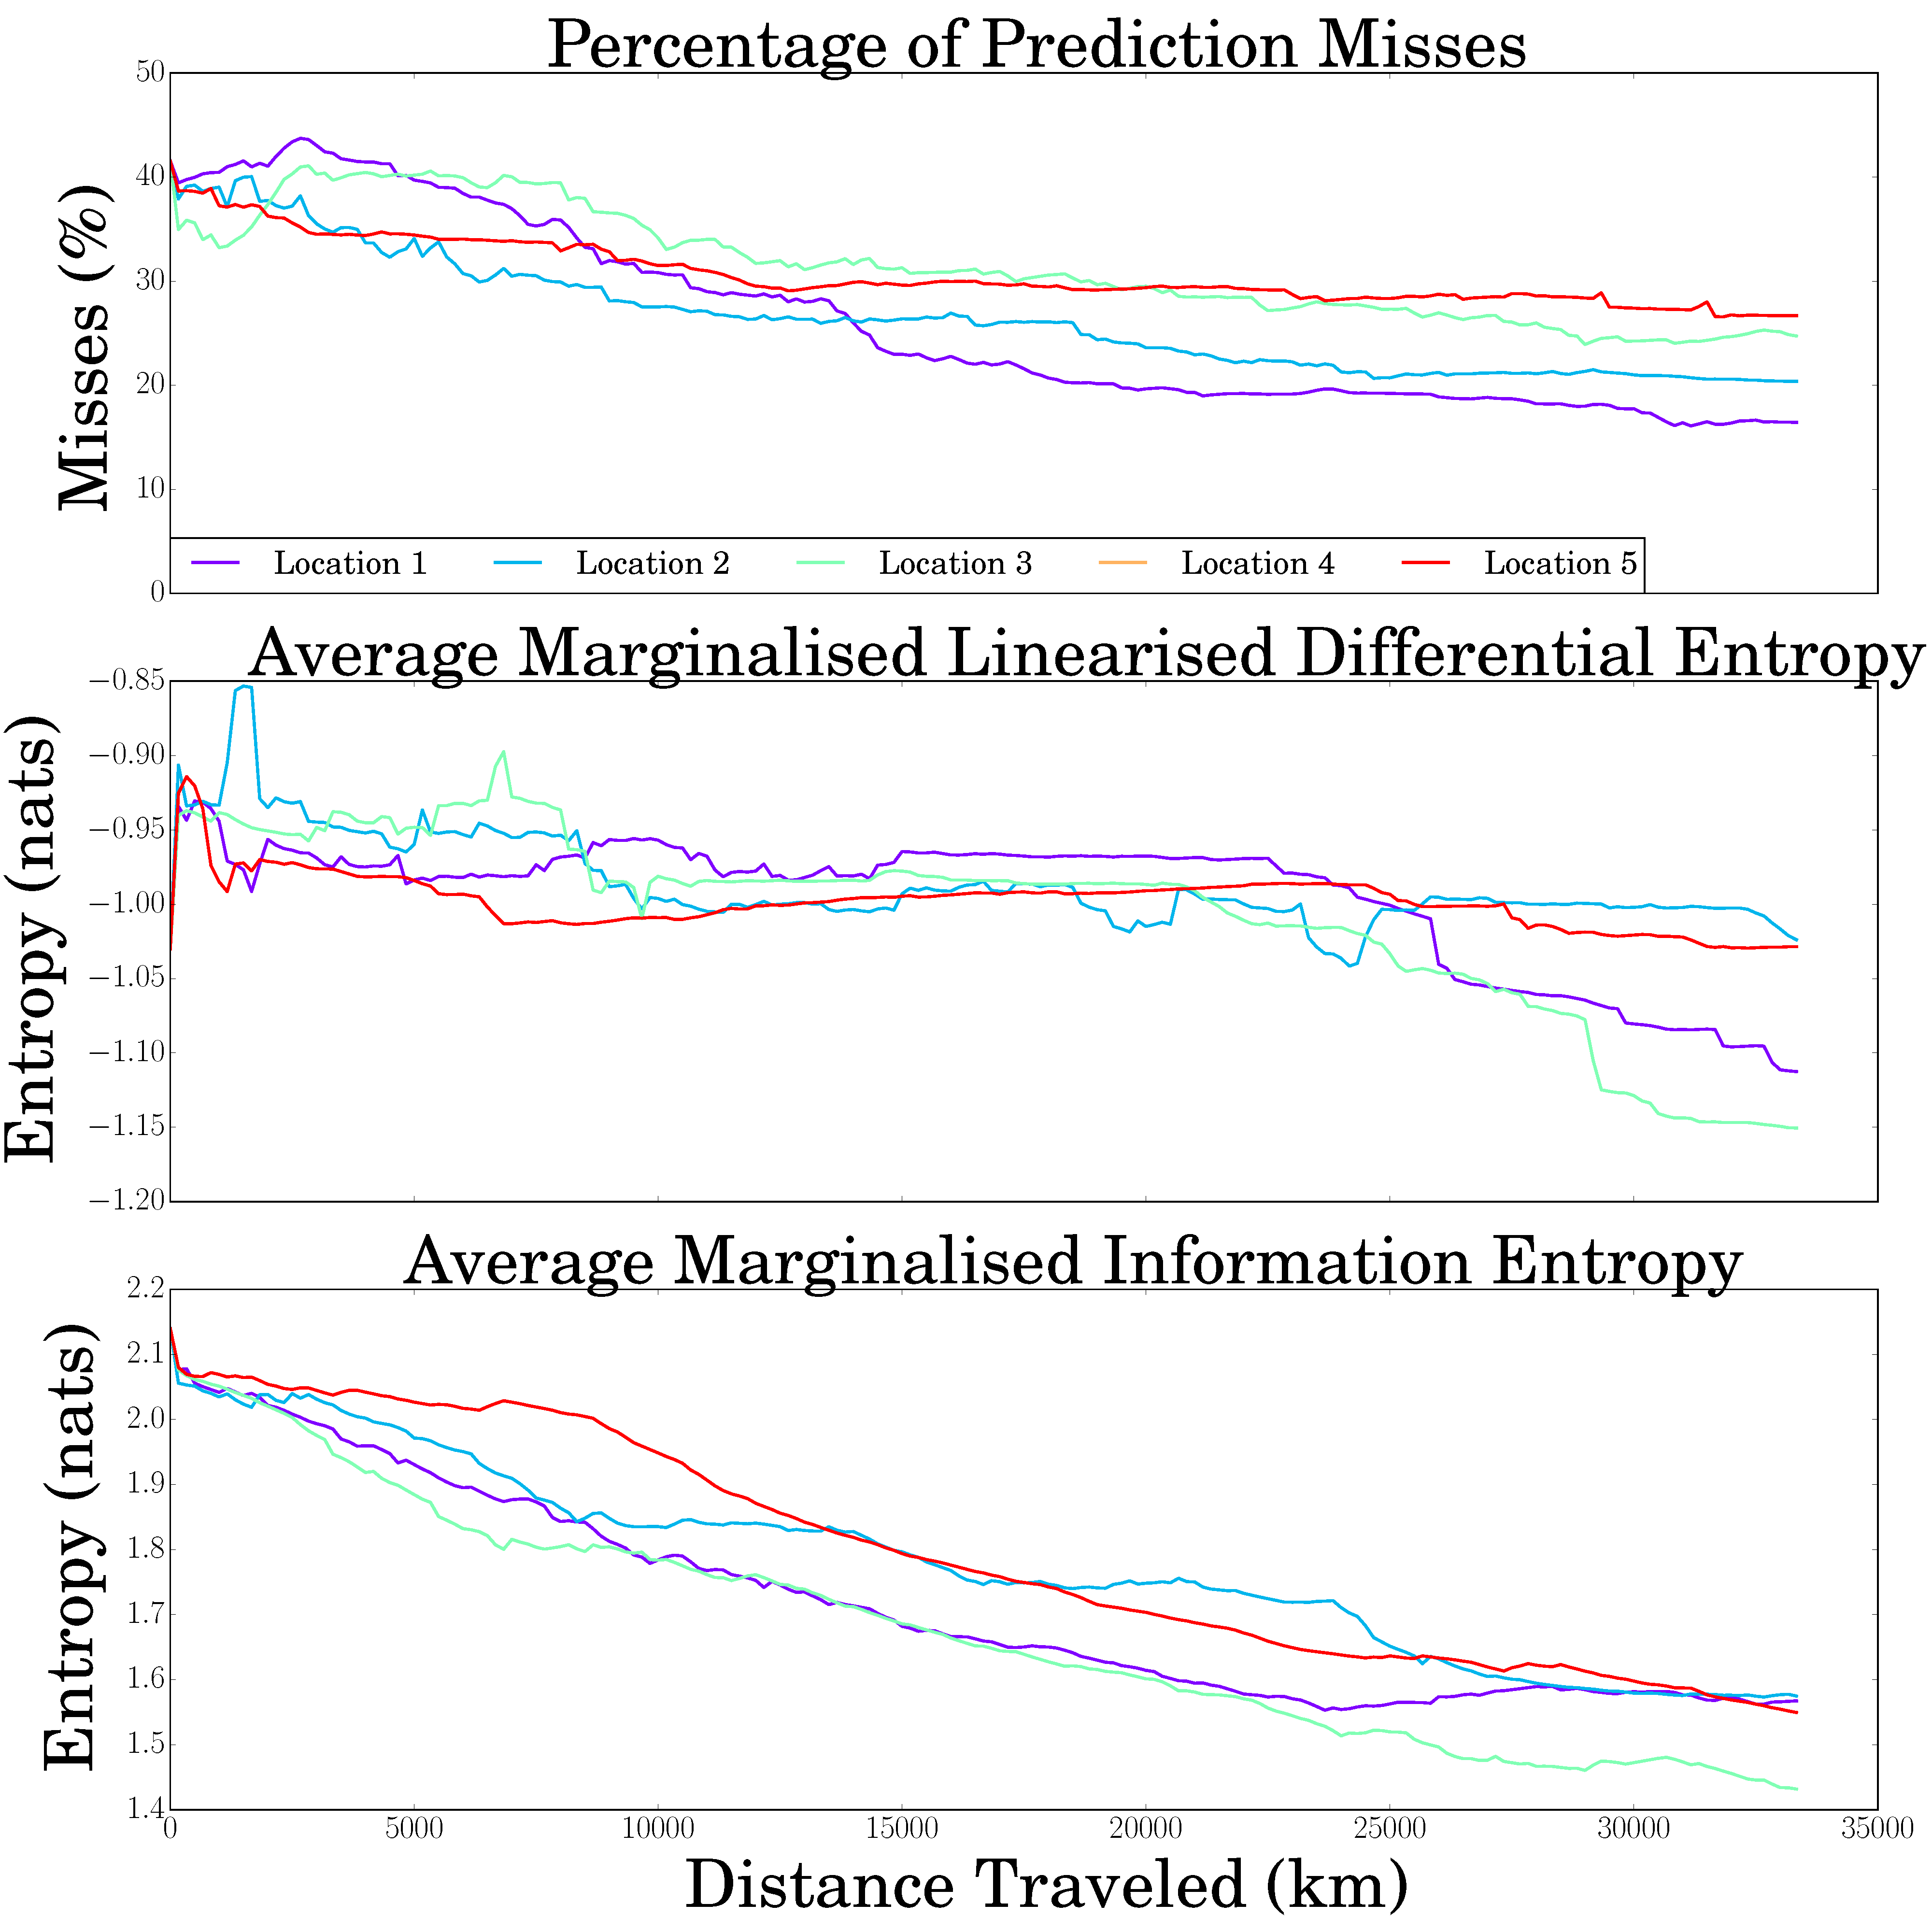
\includegraphics[width = \linewidth]{Figures/compare_locations-eps-converted-to.png}
%		\caption{Variability over starting locations}
%		\label{Figure:Results:CompareLocations}
%		\end{figure}

\section{Conclusions and Future Work}
\label{Section:Conclusion}

	In this paper we motivate, define, and derive the use of linearised differential entropy as an alternative acquisition function to informative path planning. We demonstrate the use of such an acquisition function under a receding horizon approach, and verify its performance on collected bathymetric and benthic data at Scott Reef. We show that this approach achieves lower misclassification rate experimentally in comparison to Monte Carlo methods and myopic methods.
	
	This work is ongoing and more investigation is required to fully assess the quality of LDE acquisition. Specifically, the effects of horizon length, number of control points, and the tolerances of the optimisers used should be rigorously investigated to understand robustness properties of LDE acquisition under receding horizon approach.
	
	Future investigations include extending LDE acquisition to the continuous path-planning domain. Further more, as linearised differential entropy and prediction information entropy are complementary with respect to the bias-variance trade-off, it is possible that an acquisition function that combines the two appropriately can further improve mapping accuracy.
		
\section*{Acknowledgments}

	This work is supported by the Australian Centre for Field Robotics (ACFR), the University of Sydney, and National ICT Australia (NICTA). NICTA is funded by the Australian Government through the ICT Centre of Excellence program. 
	
%% This section was initially prepared using BibTeX.  The .bbl file was
%% placed here later
%\bibliography{publications}
%\bibliographystyle{named}
%% The file named.bst is a bibliography style file for BibTeX 0.99c

\bibliographystyle{named}
\bibliography{acra2015}

\end{document}

